%%%%%%%%%%%%%%%%%%%%%%%%%%%%%%%%%%%%%%%%%%%%%%%%%%%%%%%%%%%%%%%
%% OXFORD THESIS TEMPLATE

% Use this template to produce a standard thesis that meets the Oxford University requirements for DPhil submission
%
% Originally by Keith A. Gillow (gillow@maths.ox.ac.uk), 1997
% Modified by Sam Evans (sam@samuelevansresearch.org), 2007
% Modified by John McManigle (john@oxfordechoes.com), 2015
%
% This version Copyright (c) 2015-2017 John McManigle
%
% Broad permissions are granted to use, modify, and distribute this software
% as specified in the MIT License included in this distribution's LICENSE file.
%

% I've (John) tried to comment this file extensively, so read through it to see how to use the various options.  Remember
% that in LaTeX, any line starting with a % is NOT executed.  Several places below, you have a choice of which line to use
% out of multiple options (eg draft vs final, for PDF vs for binding, etc.)  When you pick one, add a % to the beginning of
% the lines you don't want.

%%%%% LW - new command sections

\newcommand{\grun}{Gr\"{u}neisen }
\newcommand{\mob}{cm$^2$V$^{-1}$s$^{-1}$}





%%%%% CHOOSE PAGE LAYOUT
% The most common choices should be below.  You can also do other things, like replacing "a4paper" with "letterpaper", etc.

% This one will format for two-sided binding (ie left and right pages have mirror margins; blank pages inserted where needed):
%\documentclass[a4paper,twoside]{ociamthesis}
% This one will format for one-sided binding (ie left margin > right margin; no extra blank pages):
%\documentclass[a4paper]{ociamthesis}
% This one will format for PDF output (ie equal margins, no extra blank pages):
\documentclass[a4paper,nobind]{iclthesis} 

%%%%% LW - quotes
\usepackage{csquotes}

%%%%%LW - table options

\usepackage{dcolumn}% Align table columns on decimal point
\usepackage{booktabs}% introduce commands for toprule, cmidrule, bottomrule
\renewcommand{\arraystretch}{1.2}   % increase spacing between rows


%%%%% SELECT YOUR DRAFT OPTIONS
% Three options going on here; use in any combination.  But remember to turn the first two off before
% generating a PDF to send to the printer!

% This adds a "DRAFT" footer to every normal page.  (The first page of each chapter is not a "normal" page.)
\fancyfoot[C]{\emph{DRAFT Printed on \today}}  

% This highlights (in blue) corrections marked with (for words) \mccorrect{blah} or (for whole
% paragraphs) \begin{mccorrection} . . . \end{mccorrection}.  This can be useful for sending a PDF of
% your corrected thesis to your examiners for review.  Turn it off, and the blue disappears.
\correctionstrue


%%%%% BIBLIOGRAPHY SETUP
% Note that your bibliography will require some tweaking depending on your department, preferred format, etc.
% The options included below are just very basic "sciencey" and "humanitiesey" options to get started.
% If you've not used LaTeX before, I recommend reading a little about biblatex/biber and getting started with it.
% If you're already a LaTeX pro and are used to natbib or something, modify as necessary.
% Either way, you'll have to choose and configure an appropriate bibliography format...

% The science-type option: numerical in-text citation with references in order of appearance.
\usepackage[ style=nature, autocite=superscript, sorting=none, backend=bibtex, doi=false, eprint=false, isbn=false, url=true]{biblatex}
\newcommand*{\bibtitle}{References}

% The humanities-type option: author-year in-text citation with an alphabetical works cited.
%\usepackage[style=authoryear, sorting=nyt, backend=biber, maxcitenames=2, useprefix, doi=false, isbn=false]{biblatex}
%\newcommand*{\bibtitle}{Works Cited}

% This makes the bibliography left-aligned (not 'justified') and slightly smaller font.
\renewcommand*{\bibfont}{\raggedright\small}


% Change this to the name of your .bib file (usually exported from a citation manager like Zotero or EndNote).
\addbibresource{references.bib}
\addbibresource{library.bib}


% Uncomment this if you want equation numbers per section (2.3.12), instead of per chapter (2.18):
%\numberwithin{equation}{subsection}

%%%%% LW - chemical formatting
\usepackage[version=4]{mhchem}

%%%%% LW - SI units
\usepackage{siunitx}

%%%%% LW - paragraph settings
\usepackage{parskip}

%%%%% THESIS / TITLE PAGE INFORMATION
% Everybody needs to complete the following:
\title{Defects and Distortions in  \\  Hybrid Halide Perovskites}
\author{Lucy Dorothy Whalley}
\college{Department of Materials}

% Master's candidates who require the alternate title page (with candidate number and word count)
% must also un-comment and complete the following three lines:
%\masterssubmissiontrue
%\candidateno{933516}
%\wordcount{28,815}

% Uncomment the following line if your degree also includes exams (eg most masters):
%\renewcommand{\submittedtext}{Submitted in partial completion of the}
% Your full degree name.  (But remember that DPhils aren't "in" anything.  They're just DPhils.)
\degree{Doctor of Philosophy}
% Term and year of submission, or date if your board requires (eg most masters)
\degreedate{August 2019}


%%%%% YOUR OWN PERSONAL MACROS
% This is a good place to dump your own LaTeX macros as they come up.

% To make text superscripts shortcuts
	\renewcommand{\th}{\textsuperscript{th}} % ex: I won 4\th place
	\newcommand{\nd}{\textsuperscript{nd}}
	\renewcommand{\st}{\textsuperscript{st}}
	\newcommand{\rd}{\textsuperscript{rd}}

%%%%% THE ACTUAL DOCUMENT STARTS HERE
\begin{document}



%%%%% CHOOSE YOUR LINE SPACING HERE
% This is the official option.  Use it for your submission copy and library copy:
%\setlength{\textbaselineskip}{22pt plus2pt}
% This is closer spacing (about 1.5-spaced) that you might prefer for your personal copies:
\setlength{\textbaselineskip}{18pt plus2pt minus1pt}

% You can set the spacing here for the roman-numbered pages (acknowledgements, table of contents, etc.)
\setlength{\frontmatterbaselineskip}{17pt plus1pt minus1pt}

% Leave this line alone; it gets things started for the real document.
\setlength{\baselineskip}{\textbaselineskip}

%%%%% LW - paragraph options

\setlength{\parindent}{0cm}
\setlength{\parskip}{0.3\baselineskip}
%%%%% CHOOSE YOUR SECTION NUMBERING DEPTH HERE
% You have two choices.  First, how far down are sections numbered?  (Below that, they're named but
% don't get numbers.)  Second, what level of section appears in the table of contents?  These don't have
% to match: you can have numbered sections that don't show up in the ToC, or unnumbered sections that
% do.  Throughout, 0 = chapter; 1 = section; 2 = subsection; 3 = subsubsection, 4 = paragraph...

% The level that gets a number:
\setcounter{secnumdepth}{2}
% The level that shows up in the ToC:
\setcounter{tocdepth}{2}


%%%%% ABSTRACT SEPARATE
% This is used to create the separate, one-page abstract that you are required to hand into the Exam
% Schools.  You can comment it out to generate a PDF for printing or whatnot.
%\begin{abstractseparate}
%	Hybrid halide perovskites are being developed for use as an absorber material in solar cells, alongside other optoelectronic applications such as a light-emitting diode emitter or lasing material. Research interest in this material family has grown quickly over the decade, as photovoltaic efficiencies have increased from 10.9\% in 2012 to the current record of 24.2\%.  In addition, the synthesis procedure is a low-temperature solution-deposition method which, when commercialised, may lead to a reduction in solar module production prices. 

Materials theory and simulation has struggled to keep up with the rapid experimental progress as many of the physical processes that determine solar cell performance are related to defects (e.g.\ carrier capture and recombination) and temperature (e.g.\ degradation and ion migration), which are challenging to model from first-principles. Density Functional Theory (DFT) is used to predict ground-state properties only, and a typical DFT calculation for a crystalline material assumes that the material is perfectly periodic, with no point or extended defects. To model temperature effects or defects it is necessary to combine DFT with other methods, such as lattice dynamics or finite-size corrections. The aim of this PhD project is to move away from the idealised picture of a perfect material at absolute zero and towards a more realistic picture, where the defects and distortions of hybrid halide perovskites are considered.

% 10.9 from snaith paper:https://science.sciencemag.org/content/338/6107/643
% 24.2 from Solar cell efficiency tables (version 54) % Create an abstract.tex file in the 'text' folder for your abstract.
%\end{abstractseparate}


% JEM: Pages are roman numbered from here, though page numbers are invisible until ToC.  This is in
% keeping with most typesetting conventions.
%\begin{romanpages}

% Title page is created here
\maketitle

%%%%% ABSTRACT -- Nothing to do here except comment out if you don't want it.
\begin{abstract}
	Hybrid halide perovskites are being developed for use as an absorber material in solar cells, alongside other optoelectronic applications such as a light-emitting diode emitter or lasing material. Research interest in this material family has grown quickly over the decade, as photovoltaic efficiencies have increased from 10.9\% in 2012 to the current record of 24.2\%.  In addition, the synthesis procedure is a low-temperature solution-deposition method which, when commercialised, may lead to a reduction in solar module production prices. 

Materials theory and simulation has struggled to keep up with the rapid experimental progress as many of the physical processes that determine solar cell performance are related to defects (e.g.\ carrier capture and recombination) and temperature (e.g.\ degradation and ion migration), which are challenging to model from first-principles. Density Functional Theory (DFT) is used to predict ground-state properties only, and a typical DFT calculation for a crystalline material assumes that the material is perfectly periodic, with no point or extended defects. To model temperature effects or defects it is necessary to combine DFT with other methods, such as lattice dynamics or finite-size corrections. The aim of this PhD project is to move away from the idealised picture of a perfect material at absolute zero and towards a more realistic picture, where the defects and distortions of hybrid halide perovskites are considered.

% 10.9 from snaith paper:https://science.sciencemag.org/content/338/6107/643
% 24.2 from Solar cell efficiency tables (version 54)
\end{abstract}

% This is where the whole-document ToC appears:
\tableofcontents

%%%%% DEDICATION -- If you'd like one, un-comment the following.
%\begin{dedication}
%This thesis is dedicated to\\
%someone\\
%for some special reason\\
%\end{dedication}

%%%%% COPYRIGHT -- Nothing to do here except comment out if you don't want it.
\begin{copyright}
 	The copyright of this thesis rests with the author. Unless otherwise
indicated, its contents are licensed under a Creative Commons
Attribution-Non Commercial 4.0 International Licence (CC BY-NC).
Under this licence, you may copy and redistribute the material in any
medium or format. You may also create and distribute modified
versions of the work. This is on the condition that: you credit the
author and do not use it, or any derivative works, for a commercial
purpose.
When reusing or sharing this work, ensure you make the licence
terms clear to others by naming the licence and linking to the licence
text. Where a work has been adapted, you should indicate that the
work has been changed and describe those changes.
Please seek permission from the copyright holder for uses of this
work that are not included in this licence or permitted under UK
Copyright Law.
\end{copyright}

%%%%% DECLARATION -- Nothing to do here except comment out if you don't want it.
\begin{declaration}
 	I declare that this thesis and the work presented in it are my own and has been generated by me as the result of my own original research. This work has included: identifying research questions, preparing input files for calculations, submitting and monitoring calculations, writing scripts and software packages for analysis, interpreting the results and writing research papers. Where work is not my own references are given. In addition, I list below the instances where work has been done in conjunction with others.
\vspace{\frontmatterbaselineskip}

\textbf{Theory and simulation of hybrid halide perovskites } 

%The text in this chapter is largely reproduced from a published paper.\autocite{Whalley2017} The lead author is myself and co-authors are Jarvist M. Frost, Young-Kwang Jung and Aron Walsh.
The central idea of this chapter (to review the theory and simulation of hybrid halide perovskites) was provided by Aron Walsh. The contents of the review were a product of discussions between myself, Aron Walsh and Jarvist Frost. Aron Walsh prepared Figures 2.1, 2.2 and 2.4, and Young-Kwang Jung prepared Figure 2.3. This chapter is a literature review; the primary research underpinning this chapter was performed by Jarvist M. Frost (molecular dynamic and Monte Carlo investigations), Federico Brivio (crystal and electronic structure), Jonathan M. Skelton (lattice dynamics and vibrational spectroscopy), and myself (band-gap deformations).

\vspace{\frontmatterbaselineskip}

\textbf{Electronic band non-parabolicity}

%The text in this chapter is largely reproduced from a published paper.\autocite{Whalley2019} The lead author is myself and co-authors are Jarvist M. Frost, Benjamin J. Morgan and Aron Walsh. 
The initial research direction (to investigate, across a range of photovoltaic materials, the sensitivity of DFT calculated effective mass to fitting parameters) was provided by Aron Walsh and Benjamin Morgan. Jarvist Frost suggested weighting the fit to a Fermi-Dirac distribution. 

\vspace{\frontmatterbaselineskip}

\textbf{Electron-phonon and phonon-phonon coupling}

%The text in this chapter combines results from two published papers.\autocite{Whalley2016,Whalley2017a} The lead authors are myself\autocite{Whalley2016} and Jarvist M. Frost,\autocite{Whalley2017a} and the co-authors are Jonathan M. Skelton and Aron Walsh. 
Jarvist Frost suggested using a classical heat diffusion model for hot carrier cooling and calculated the temperature dependent bandgap shifts. Jonathan M. Skelton provided scripts to implement the frozen phonon method. Aron Walsh prepared Figure 5.1.

\vspace{\frontmatterbaselineskip}

\textbf{Electron trapping at H-centre defects}

% ADJUST BELOW
%The text in this chapter includes work from a published paper.\autocite{Whalley2017b} The lead author is myself and co-author is Aron Walsh. 
The central idea of this chapter (to investigate hole capture at an iodine interstitial in \ce{CH3NH3PbI3}) was provided by Aron Walsh. Sunghyun Kim and Samantha Hood provided early (pre-publication) access to the software package \textsc{CarrierCapture.jl}, which I used to analyse the data presented in Section \ref{ch:6-results}. Aron Walsh prepared Figures 1.3a and 1.3c. The energies of the H-centre optically excited states were calculated by Rachel Crespo-Otero.
\end{declaration}

%%%%% LW - publications
\begin{publications}
 	
The following publications have arisen from this PhD work. Where copyright is retained by the publisher, text and figures are reprinted with permission, as detailed in Appendix \ref{app:5-copyright}.

\vspace{\frontmatterbaselineskip}

\textbf{Theory and simulation of hybrid halide perovskites } 

Text and figures 1--4 reprinted from
\href{https://doi.org/10.1063/1.4984964}{Whalley, L. D., Frost, J. M., Jung, Y. -K. and Walsh, A. (2017). Perspective: Theory and simulation of hybrid halide perovskites. \textit{The Journal of Chemical Physics}, 146(22), p.220901.} © 2017 CC-BY
\vspace{\frontmatterbaselineskip}

\textbf{Electronic band non-parabolicity}

Text and figures 1--11 reprinted from
\href{https://doi.org/10.1103/PhysRevB.99.085207}{Whalley, L. D., Frost, J., Morgan, B. and Walsh, A. (2019). Impact of nonparabolic electronic band structure on the optical and transport properties of photovoltaic materials. \textit{Physical Review B}, 99(8).} © 2019 American Physical Society
\vspace{\frontmatterbaselineskip}

\textbf{Electron-phonon and phonon-phonon coupling}

Excerpts and figures 2--4 reprinted from
\href{https://doi.org/10.1103/PhysRevB.94.220301}{Whalley, L. D., Skelton, J. M., Frost, J. M. and Walsh, A. (2016). Phonon anharmonicity, lifetimes, and thermal transport in \ce{CH3NH3PbI3} from many-body perturbation theory. \textit{Physical Review B}, 94(22).} © 2016 American Physical Society

Excerpts and figures 1,5--6 reprinted from
\href{https://doi.org/10.1021/acsenergylett.7b00862}{Frost, J. M., Whalley, L. D and Walsh, A. (2017). Slow Cooling of Hot Polarons in Halide Perovskite Solar Cells. \textit{ACS Energy Letters}, 2(12), pp.2647-2652.} © 2017 CC-BY
\vspace{\frontmatterbaselineskip}

\textbf{Electron trapping at H-centre defects}

Excerpts reprinted from
\href{https://doi.org/10.1021/acsenergylett.7b00995}{Whalley, L. D., Crespo-Otero, R. and Walsh, A. (2017). H-Center and V-Center Defects in Hybrid Halide Perovskites. \textit{ACS Energy Letters}, 2(12), pp.2713-2714.} © 2017 American Chemical Society 
\vspace{\frontmatterbaselineskip}

\textbf{Appendix C: effmass: An effective mass package}

Text reprinted from
\href{https://doi.org/10.21105/joss.00797}{Whalley, L. D. (2018). effmass: An effective mass package. \textit{Journal of Open Source Software}, 3(28), p.797.} © 2018 CC-BY 



\end{publications}

%%%%% ACKNOWLEDGEMENTS -- Nothing to do here except comment out if you don't want it.
\begin{acknowledgements}
 	Leaving an enjoyable job and returning to study is not an easy decision, but starting a PhD in the Walsh group was one of the best I have made. A huge thanks must be given to Aron Walsh for creating and maintaining a supportive, friendly and productive working environment. I have gained a \textit{huge} amount from working with Aron and other members of the group. Although I have learnt something from every member I will not list everyone here, but a special thanks must go to Jarvist Frost who led the book group and helped clarify my sometimes muddled understanding of solid state physics. Another special thanks to the women I have worked with: we are still too few and far between in the physical sciences, but what we lack in quantity we make up for in quality! Thanks also to Benjamin Morgan, my second supervisor, who guided me through my first research project and has provided useful feedback on my scientific writing. 

During the third year of my PhD I became involved with the Research Software Engineering community at Imperial. I would like to thank Katerina Michalickova for organising the Software Carpentry workshops -- it is no easy job co-ordinating a rabble of volunteers from across Imperial, but teaching software carpentry has greatly increased my confidence around programming. Thanks also to fellow members of the Imperial RSE community committee, especially Jeremy Cohen who is mentoring me as part of my Software Sustainability Institute fellowship.

The vast majority of the computational analysis in this thesis depends to some degree on the open-source community. Thousands of person-hours, often I suspect squeezed in at weekends or evenings, has produced well-tested, well-documented, easily accessible code. Without the magical Python `import` statement and the generosity of strangers I would probably still be writing an integration routine for my first year project. I have referenced the domain-specific software packages used throughout the main text of this thesis, but here I must acknowledge the general-purpose software tools I have used: Python and Julia for scripting, the scientific Python stack (Numpy, Scipy, Pandas, Matplotlib, Pytest and Jupyter) for data analysis, testing and plotting, Sphinx and ReadTheDocs for documentation, Vim and Sublime for text editing, Git for version control, and LaTeX for type setting.

Thanks also to the admin and technical staff who keep the supercomputers Archer, Thomas and Piz-Daint running. I rarely think about the infrastructure behind my calculations, and this is exactly why I need to say thanks.

Funding for my PhD came from the EPSRC, via the Centre for Doctoral Training in New and Sustainable Photovoltaics. It seems that running a CDT requires staff to go above and beyond - thanks to Ken Durose, Alison Walker, Rob Treharne and Asim Mumtaz for doing just that.

The biggest thanks must go to my family and friends. I met Richard towards the start of my PhD. It is now four years on, and we have bought a house, got married and created a very small human being (currently still residing in my tummy). I wouldn't have expected that all this was compatible with doing a PhD, but being with Richard has made it seem like the most natural thing in the world. He has been with me, and supported me, throughout. It is through Richard's parents, Andrew and Elspeth, that I was introduced to John and Karen. By gifting me the use of their flat twice a week for three years, John and Karen enabled me to live in Birmingham and work in London. I don't think it would have been possible for me and Richard to `settle down' otherwise and for this I am very grateful.

I'm lucky to have close, reliable and hilarious friends who are always suggesting things to take my mind off work. Thanks especially to Hetta and Blanche for Lipsync and our other ``projects'', and Caz for her loyalty and warmth. Ruby, my sister, is also a close friend who understands me (and sees through me!) in a way that no-one else can. Finally, thank you to my parents John and Alison, whose love and support instilled in me a self-confidence that I think is so important when doing science. All of my achievements are theirs, as none of this would have been possible without their belief in me.
\end{acknowledgements}



%%%%% MINI TABLES
% This lays the groundwork for per-chapter, mini tables of contents.  Comment the following line
% (and remove \minitoc from the chapter files) if you don't want this.  Un-comment either of the
% next two lines if you want a per-chapter list of figures or tables.
\dominitoc % include a mini table of contents
%\dominilof  % include a mini list of figures
%\dominilot  % include a mini list of tables

% This aligns the bottom of the text of each page.  It generally makes things look better.
\flushbottom



\listoffigures
	\mtcaddchapter
	
\listoftables
    \mtcaddchapter
% \mtcaddchapter is needed when adding a non-chapter (but chapter-like) entity to avoid confusing minitoc

% Uncomment to generate a list of tables:
%\listoftables
%	\mtcaddchapter

%%%%% LIST OF ABBREVIATIONS
% This example includes a list of abbreviations.  Look at text/abbreviations.tex to see how that file is
% formatted.  The template can handle any kind of list though, so this might be a good place for a
% glossary, etc.
% First parameter can be changed eg to "Glossary" or something.
% Second parameter is the max length of bold terms.
\begin{mclistof}{Abbreviations}{3.2cm}

\item[AM] Air Mass
\item[CBM] Conduction Band Minimum
\item[CZTS] Copper zinc tin sulfide
\item[DFT] Density Functional Theory
\item[GGA] Generalised gradient approximation
\item[HF] Hartree-Fock
\item[HSE06] Heyd-Scuseria-Ernzerhof screened hybrid DFT functional 
\item[LDA] Local density approximation
\item[PBE, PBEsol] Perdew-Burke-Ernzerhof DFT functional; PBEsol is recommended for solids
\item[MAPI] Methylammonium lead iodide
\item[PV] Photovoltaic
\item[SRH] Shockley-Reed-Hall 
\item[SoC] Spin-orbit coupling
\item[VBM] Valence Band Maximum

\end{mclistof} 


%%%%% LIST OF symbols
% First parameter can be changed eg to "Glossary" or something.
% Second parameter is the max length of bold terms.
\begin{mclistof}{List of Symbols}{3.2cm}

% greek letters are the in order??
\item[$\nabla$] Vector differential operator
\item[$\epsilon$] Energy of a state
\item[$\epsilon_0$] Static dielectric constant
\item[$\epsilon_{\inf}$] High frequency (optical) dielectric constant 
\item[$\eta$] Photovoltaic efficiency
\item[$\mu$] Chemical potential
\item[$\nu$] Phonon frequency
\item[$\pi$] Pi constant $\sim 3.14$
\item[$\rho$] Electron density
\item[$\sigma$] Carrier capture cross section
\item[$\tau$] Carrier lifetime
\item[$\phi$] Kohn-Sham orbital

% greek upper
\item[$\Psi$] Many-body Wavefunction

//
% need to include all wavefunction stuff

%roman lower
\item[$e$] Exponential constant $\sim 2.72$
\item[$h$] Planck constant $\sim 6.63\times10^{-34}\textrm{Js}$
\item[$\hbar$] Reduced Planck constant $\frac{h}{2\pi}$ 
\item[$k$] Wavevector associated with periodic electronic structure
\item[$k_B$] Boltzmann constant $\sim 1.38\times10^{-23}\textrm{JK}^{-1}$
\item[$m$] Mass   % include all effective mass definitions?
\item[$n$] Carrier density
\item[$n_e$] Electron density
\item[$n_h$] Hole density
\item[$n_i$] Intrinsic carrier density
\item[$p$] Density of holes
\item[$\textbf{r}$] position vector
\item[$t$] Time
\item[$v$] Group velocity

//

% roman upper 
\item[$E$] Total energy
\item[$E_0$] Ground state energy
\item[$E_F$] Fermi energy
\item[$FF$] Fill factor
\item[$J$] Current
\item[$J_{SC}$] Short circuit current
\item[$N_t$] Trap density
\item[$P$] Power
\item[$R$] Resistance
\item[$T$] Temperature
\item[$V$] Voltage
\item[$V_{OC}$] Open circuit voltage


\end{mclistof} 

% The Roman pages, like the Roman Empire, must come to its inevitable close.
%\end{romanpages}



%%%%% CHAPTERS
% Add or remove any chapters you'd like here, by file name (excluding '.tex'):
\flushbottom
\begin{savequote}[8cm]
For generations, we have assumed that the efforts of mankind would leave the fundamental equilibrium of the world's systems and atmosphere stable. But it is possible that with all these enormous changes (population, agricultural, use of fossil fuels) concentrated into such a short period of time, we have unwittingly begun a massive experiment with the system of this planet itself.
  \qauthor{--- Margaret Thatcher}
\end{savequote}

\chapter{\label{ch:1-intro}Introduction} 

\minitoc

\section{Motivation}

In this section I justify photovoltaic materials research. First, the challenge we face as a human race -- global warming -- is introduced, followed by why we should take advantage of the sun as an energy source. The section ends with a discussion about the three generation of solar cell materials, and the inherent limitations of silicon solar cells.

\subsection{Energy use and global warming}

%The IPCC models have 5 things which need to happen in all scenarios. one of them is the reducition in energy output which we are doing. but must happen in conjunction with others.
Anthropogenic climate change is one of the greatest challenges we face as a human race and, as we have twelve years to limit climate change catastrophe, we are running against the clock. This viewpoint is not party political or the political hyperbole of the green left, as I have tried to allude to with the opening quote -- this is the current scientific understanding as established by the International Panel on Climate Change.\autocite{IPCC2018}

The story begins in the 18th century when the industrial revolution enabled unprecedented population growth, from 0.8 billion in 1750 to 7.5 billion in 2017.\autocite{Kaneda2017}
Industrial expansion combined with a growing population led to an exponential growth in the amount of coal and oil being burnt; between the years 1769 and 2006 there was an 800-fold increase in the world annual coal production.\autocite{MacKay2009}
Atmospheric \ce{CO2} concentrations increased as a result, leading to an increase in global temperatures, rising sea levels, and ocean acidification. The years 2014--2018 were the five hottest years on record \autocite{gistemp2018} and there has been a recent increase in extreme weather (heat waves, drought and floods) across the globe.\autocite{easac2018} Studies have shown that the probability of heat waves,\autocite{Black2016} wildfires\autocite{Abatzoglou2016} and flooding \autocite{Sweet2016,vanderWiel2017} have increased as a result climate change.

The threat of climate change seems not to have had a proportionate response from governments or many individuals. One reason for this is that changes in weather patterns are significant only when looked at over long time periods, and so it is difficult to communicate the risk carried by climate change. Another is that this is an inherently international problem, and that we do not have the political mechanisms in place to coordinate a global response. Despite the dramatic consequences of inaction, there seems to be little public appetite for changes which require a reduction in energy use. Instead there is a push towards technological solutions which may be able to reduce the negative effects of climate change without impacting upon our perceived quality of life.

%\begin{figure}[h]
%\centering
%  \includegraphics[width=0.5\columnwidth]{C01/figs/ag.png}
%  \caption[XKCD comic - climate change]{The XKCD comic character suggests that the timescales of climate change can lead to the perception that there is no climate change; like an electron an adiabatic potential, our environment changes and we simply adjust with it. Reproduced with permission from \url{https://xkcd.com/1321/}.} %like an electron under adiabatic, we may undergo a dramatic phase change without even being aware of it.
%  \label{xkcd}
%\end{figure}

%- 1979 : 1st world climate conference. 1990: 0.3 degree rise per decade, 1995: the balance of evidence suggests discenible huma influence on global climate. 1997 - kyoto protocol.

%- Toronto July 1988: Climate change is a serious challange, undertake actions to reduce, enhance research to reduce uncertainty.


%- 2015 : agreement to limit global temp to 2C or 1.5C if posible and net zero emissions by end of century

\subsection{The sun as an energy source}
One way to reduce the rate of climate change is to generate energy through processes that do not release net positive amounts of CO$_2$ into the atmosphere, and harnessing the vast amount of energy that is released from the sun is one way of doing this. This idea has been around for more than sixty years; in 1954 Bell Labs demonstrated that it was possible to convert sunlight into electricity by powering a small toy Ferris wheel and radio transmitter with a silicon solar cell. Reporting this event, The New York Times wrote:
%http://www.aps.org/publications/apsnews/200904/physicshistory.cfmthe New York Times wrote that:
\begin{displayquote}
“[the solar cell] may mark the beginning of a new era, leading eventually to the realization of one of mankind’s most cherished dreams –- the harnessing of the almost limitless energy of the sun for the uses of civilization.”
\end{displayquote}
A solar flux density of $1361\,\textrm{Wm}^{-2}$ reaches the earth's atmosphere each second, which is almost $10^4$ times larger than any other external energy source.\autocite{Kopp2011} A quick back-of-the-envelope calculation shows that if we assume a sunlight to electricity conversion efficiency of 40\% (achievable using concentrated solar power) and zero transmission loss, we could meet the world's electricity demands ($22\,\textrm{PWh}$ in 2015\autocite{IEA2017}) by covering an area equivalent to Northumberland county ($5000\,\textrm{km}^2$) with photovoltaic solar panels.
%$46400\,Wm^{-2}$ is the absolute limit if we consider concentrator cell architectures (section \ref{SQlimit}). 
%
%The cost of PV installations is increasingly due to the infrastructure around the solar cell: for example, module encapsulation and installation\autocite{Green2016}. As a consequence, improving the efficiency of a device is the way to lower costs: with an increasing efficiency, a decreasing area is required to produce an equal amount of power, and all of the costs that scale with area are reduced. For new devices to succeed they must be able to match or exceed the efficiency of silicon.
However to harness this power we must be able to convert sunlight into electrical energy at a competitive price and at scale. Photovoltaic efficiency is key to price reduction as there are significant costs that scale with area,\autocite{Fraunhofer2015,Green2016} and a higher efficiency module can deliver the same energy for a smaller area.

The first photovoltaic devices could transform sunlight into electrical energy with an efficiency of around 6\%. The computing boom of the 1980s encouraged large investment into silicon research and  silicon cells with 20\% efficiency were reported in 1986.\autocite{Blakers1986} Since 1980 costs have decreased at an average rate of 10\% per year\autocite{Farmer2016} (Fig.\ \ref{module_price}) and the global market is growing, from a capacity of 1.9 GW in 2005 to 102 GW in 2016.\autocite{Jager-Waldau2017}

\begin{figure}[h]
\centering
  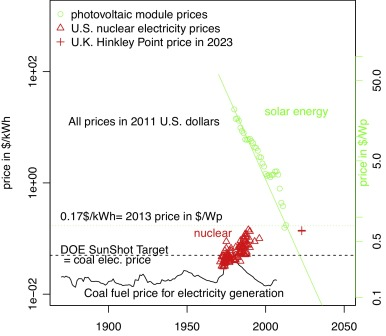
\includegraphics[width=0.6\columnwidth]{figures/ch1/solarcost.jpg}
  \caption[Historic and predicted costs of solar energy generation]{Historic and predicted costs of energy generation. The cost of solar energy (green) has been decreasing exponentially (at an average rate of 10\% per year) and is now comparable with the cost of energy generated from nuclear power (red). The dashed line corresponds to a  solar energy cost target from the US Department of Energy of \SI{0.05}{\$\per\kilo\watt\hour}. Reproduced with permission from the work of Farmer et al.\autocite{Farmer2016}}
  \label{module_price}
\end{figure}
% https://www.ise.fraunhofer.de/content/dam/ise/de/documents/publications/studies/AgoraEnergiewende_Current_and_Future_Cost_of_PV_Feb2015_web.pdf
% http://energy-age.blogspot.com/2015/02/pv-price-in-future.htmlf
% https://www.greentechmedia.com/articles/read/pv-solar-costs-have-fallen-10-per-year-since-1980#gs.HkfY3X4
% Schematic idea: GWP installed per year as a funnel (bottmoo 1980, top currrent) but also split into colour by material type. Shows growth in diversity as well as overall.
% the levelized cost of energy by PV has dropped dramatically: see schematic: WEF Renewable Infrastructure Investment Handbook
% https://openei.org/apps/TCDB/transparent_cost_database THIS IS A GREAT DATABASE FOR COMPARISON - use to generate own version of the schematic in WEF
%- 100MW in china is largest installed, top solar plants: http://www.pvresources.com/en/top50pv.php

In the UK the growth in renewable energy has led to a decreasing dependence on fossil fuels. The UK had it's first day without coal in 2017\autocite{Brown2017} and ran for three days without coal in 2018.\autocite{Vaughan2018} There appears to be a growing political will to take advantage of renewable energy; the first UK National Infrastructure Assessment recommends halting the development of nuclear power stations and diverting investment into solar and wind energy generation instead.\autocite{NIA2018} This switch away from nuclear energy is projected to be at no cost to the consumer.

It is widely predicted that solar power will continue to grow -- to what extent depends on the source: a recent study from Imperial College London estimates that solar power could supply 23\% of global energy demand in 2040.\autocite{Grantham2017} ExxonMobil, a company heavily invested in fossil fuels, predicts that all renewables combined will supply 20\% of global power generation in 2040.\autocite{exxon2018} Note that previous models have consistently underestimated the scale of photovoltaic deployment.\autocite{Creutzig2017}
 % - Future : looking to terawatt.  DOI: 10.1126/science.aal1288

\subsection{Beyond silicon: the need for new photovoltaic materials}

%- from library: Photovoltaic Solar Energy: From Fundamentals to Applications: Angèle Reinders, Pierre Verlinden, Wilfried van Sark, Alexandre Freundlich
Photovoltaic devices are commonly split into three generations. In this section I introduce each generation and discuss what is driving the development of new PV materials in a competitive market that is dominated by silicon.

\textbf{First generation}

The first generation devices are based upon mono- and poly-crystalline silicon wafers. They dominate the PV market; in 2016 90\% of total PV module production used this technology.\autocite{Jager-Waldau2017}. They are high efficiency (>20\%), reliable (25 year lifetimes) and low cost (<0.5 \$/W). There has been a steady decrease in cost due to i) device engineering improvements (eg: textured surfaces); ii) the economies of scale as silicon industrial processes are driven by a demand for computer chips; and iii) improved industrial practices which allow thinner and thinner wafers to be fabricated with less waste. However there are technological and physical limits to how much the cost of a crystalline silicon wafer can be reduced. First, the manufacturing process for silicon wafers is energy intensive and requires high temperatures. Second, silicon is an indirect bandgap material and as a result does not absorb sunlight efficiently; wafers have to be a minimum thickness ($\sim 60\mu \textrm{m}$) to compensate for this. It is difficult to reach this limit without snapping the material during fabrication as silicon is a hard and brittle material.

\textbf{Second generation}

Second generation devices are fabricated from the direct bandgap materials gallium arsenide (GaAs), cadmium telluride (CdTe), cadmium indium gallium diselenide (CIGS) and amorphous silicon (a-Si). These materials have higher absorption coefficients, so they can be built into lighter thin-film ($\sim 10\mu \textrm{m}$) architectures. A thin-film is not mechanically stable, it needs a substrate, but this opens up possibility of it being a flexible film.

CdTe was the first thin film to be commercialised and development has been led by the company First Solar, who have installed a total capacity of \SI{17}{\giga\watt}. Lifecycle assessments indicate that the CdTe energy payback time (the time required to generate as much energy as is consumed during production and lifetime operation of the system) is shorter than that of Si.\autocite{Koppelaar2017} However lower efficiencies are stifling the growth of this technology and there are also concerns about the elemental toxicity and scarcity. CIGS and a-Si each have a smaller market share than CdTe. High efficiency ($\sim 40\%$) GaAs devices have been developed for the high-value, low-volume space market.

% Much is invested into cheap solution deposition methods rather than expensive vacuum deposition like that used for GaAs. Jake Bowers / Mitzi
% What about GaInP??

\textbf{Third generation}

Third generation devices are emerging technologies which are not yet in the market. This includes organic and dye-sensitised materials, hybrid halide perovskites, and copper zinc tin sulfide (CZTS). These are abundant materials which can be fabricated through low-cost solution-deposition methods. Only the hybrid-halide perovskites have efficiencies high enough for commercialisation (currently 24.2\%).

For the third generation materials commercial success may come from opening up new markets rather than trying to compete directly with well established silicon technologies. For example, organic and hybrid perovskite technologies have tunable bandgaps and are being developed for semi-transparent building integrated photovoltaics.
There has also been recent research interest and commercial investment into silicon-perovskite single junction tandem cells.
%% DEFO need to expand this. Silicon has solved the PV problem pretty much. Perovskite needs to be stable, it potentially needs to NOT have lead (though actual environmental toxicity impact is low, legislation does not reflect this), and ideally a tunable (wider) bandgap.

%% all films more the 20% have been based on diamond. All FCC - even CZTS is double ZB. APART from perovskite!!

%%perovskite is basically comparable to silicon but stability is the issue. Needs to compete on price and efficiency.

%% PV is less than coal and gas in sunnier places

%% FAPI and CsPbI are not stable perovsite structure at RT, but by mixing large and small to get an average size you get a stable structure.

%% grain size of perovskite influences stability but not immediate efficiency.

%% should really emphasise the role of defects in degradation of the device.
%% MAPI has minimum toxicological impact. (plus compare to GaAs) - most comes from silicon. Pb is very scalable. 

%Inernational technology roadmap 2017 lays out growth in tandem cells. For a large market. This is the target. should be a perovskite module made in 2019.

%- http://www.sciencedirect.com/science/article/pii/S0306261917311339 : BIPV with perovskites
%-BIPV: functionalising buildings. Generating and storing energy. Make more than need: store in car which becomes a battery on wheels which then could feed into rest of house (people use car on average one hour per day). buildings as power stations - specific - low energy wireless device
%- This is what Dyesol company want to do. They are not going to compete with silicon on the arrays of solar farms. Going to look into market where silicon has not penetrated: where it cannot because of need to be solid single crystal. Aim is functionalisation of buildings with PV. Printing on steel.

\section{Key concepts in photovoltaics}

This section outlines the physical principles underlying solar cell operation, with a focus on carrier recombination. After introducing the key concepts and vocabulary, the design rules or ``wish list'' for a successful PV material are outlined. 
%Focus upon how we can design high-efficiency materials.

\subsection{Operating principles} \label{operatingprinciples}

% % use solar cat book images

A solar cell converts light into electricity through the following (simplified) process: i) a photon enters the device; ii) the photon is absorbed and creates an electron-hole pair in the absorber layer; iii) the electron and hole disassociate; iv) the electron and hole travel through the absorber layer to their respective contacts; v) the electron and hole are extracted to the external circuit to do electrical work.

\subsubsection{Device architecture}
The device architecture is determined by the properties of the absorber material. For example, in a hybrid halide perovskite material the photogenerated electron and hole are loosely bound to one another and thermal energy is enough to separate them. In this case, a planar $n$-$i$-$p$ architecture can be used, where $n$ is a n-type (electron-doped) material contacted to the cathode, $p$ is a p-type (hole-doped) material contacted to the anode and $i$ is the intrinsic (undoped) perovskite material (Figure\ \ref{SC_architecture}). In contrast, the photogenerated electron-hole pair in an organic solar cell is strongly bound. In this case, the electron-hole pair disassociate only at an interface and a mesoscopic architecture is used to facilitate this (Figure\ \ref{SC_architecture}). The conventional organic architecture is $p$-$i$-$n$, where the anode and p-type material are deposited onto the substrate first. The conventional architectures can be inverted to give $p$-$i$-$n$ junctions (for inorganic / hybrid absorber layers) or $n$-$i$-$p$ junctions (for organic absorber layers). In all cases, the n-type and p-type layers provide a built-in electric field that drives photogenerated electrons towards the cathode material and photogenerated holes towards the anode.
% pn junction sketch.
% see https://www-ssrl.slac.stanford.edu/content/science/highlight/2011-01-31/effects-thermal-annealing-morphology-polymer%E2%80%93fullerene-blends-organic and Late Stage Review pic
% an electron transport material (eg: TiO$_2$) acting as n-doped layer and a hole transport material (eg: Spiro-MeOTAD) acting as a p-doped layer.
% work function of p-type material is larer than work function of n-type material, and the charge carriers distribute so that the fermi level is continuous across the material.

\begin{figure}[h]
 \centering
   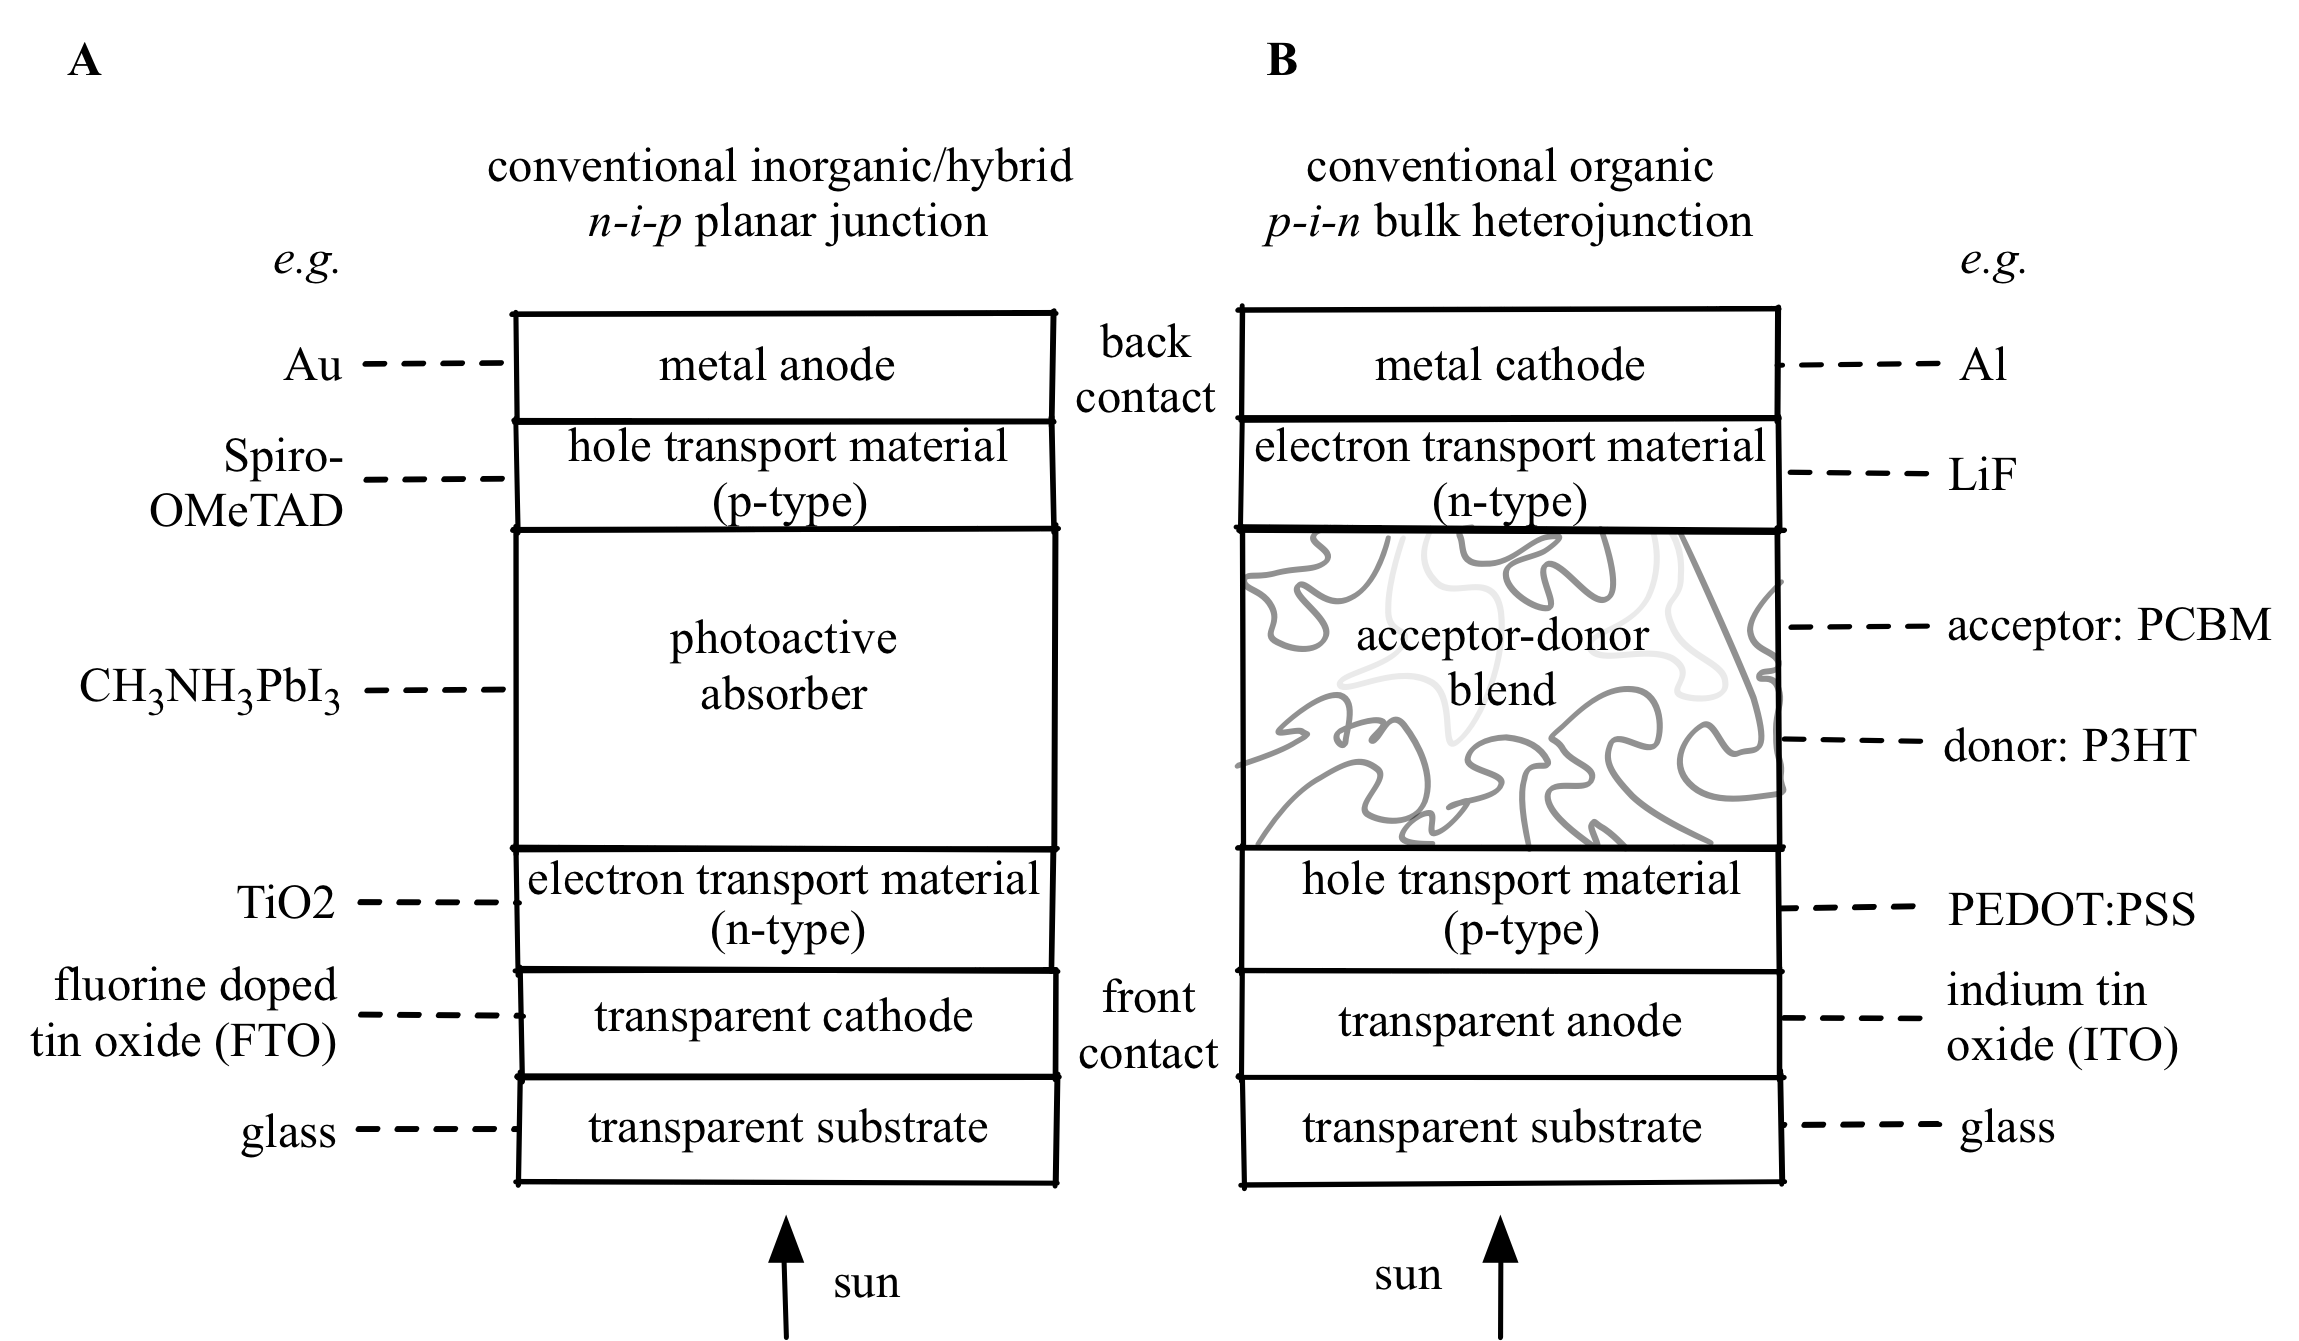
\includegraphics[width=1.0\columnwidth]{figures/ch1/PVarchitecture.png}
   \caption[Typical solar cell architectures]{(A) Schematic of the typical planar junction solar cell architecture used for an inorganic or hybrid material absorber layer (B) Schematic of the typical bulk heterojunction solar cell architecture used for an organic absorber layer. The mesoscopic architecture provides many interfaces where the electron-hole pair can disassociate.  In both cases there is a built-in electric field that drives photogenerated electrons towards the electron transport material and holes towards the hole transport material.}
   \label{SC_architecture}
 \end{figure}
% good info on organic cells here: https://www.sciencedirect.com/science/article/pii/S0038092X13003885

% %Can have multiple architectures for the same material.
% %Two types of device architecture used in commercial MAPI cells:
% % 2009: a perovskite dycell developed by miyasaka (liquid based DSSC architecture), 2013 planar thin film solid state solar cell by Snaith and graetzel( this showed standard semiconductors)
% %Planar (Snaith et al have dabs on it)
% %Mesoporous: which is said to be better re: hysterisis

%% could include here a section on "why does electrons flow toward n-type and holes towards p-type? include plot of band bending as a result of workfunctions in n-type and p-type materials and where the fermi levels are (near VBM ptype, near CBM -type) and the fact that the fermielvels must aligh.

Various strategies exist to increase device efficiency via device architecture engineering. For example, the current world record single junction silicon cell ($\eta=26.6\%$) has an additional wide bandgap material inserted between the absorption layer and contact material to reduce interfacial recombination, and interdigitated back contacts to reduce optical loss.\autocite{Yoshikawa2017} The most efficient solar cells ($\eta=46.0\%$) combine a multiple pn-junction (tandem) architecture with a lens to concentrate the incoming sunlight.

% %Adapting the device architecture can lead to large gains in efficiency. 
% % what have we learnt from Si
% %Buffer layers are used to 
% %- a lot of improvements come from tweaking the device:
% %- Inverted structures so defects do not proparagete.
% %- space layers and surface roughness to improve efficiency - engineering approaches
% %-  Remember most crriers generated near surface. Window is to stop carrier reaching surface

\subsubsection{Efficiency and reciprocity}
% %need to cite Nelson
For an external circuit with load $R$, a current $I$ and voltage $V$ is developed across the cell so that
\begin{equation}
    V = IR.
\end{equation}
$I$ and $V$ are related by a current-voltage curve (Figure\ \ref{current_voltage}).
A solar module operates at the maximum power point $P_m$, which is where the product of the voltage and current is maximum:
\begin{equation}
    P_\textrm{m}  = I_\textrm{m} V_\textrm{m}.
\end{equation} 
The open-circuit voltage $V_{\textrm{oc}}$ is the voltage produced when there is no contact to the external circuit (or, equivalently, the external circuit has an infinite load). 
The short-circuit current $I_{\textrm{SC}}$ is the current that flows when there is no load on the external circuit.
The fill factor FF is defined as:
\begin{equation}
    \textrm{FF} = \frac{I_\textrm{m}V_\textrm{m}}{I_\textrm{sc} V_\textrm{oc}}.
\end{equation}
The higher the fill factor, the higher the maximum powerpoint for a given $V_\textrm{oc}$ and $I_\textrm{sc}$.\autocite{Nelson2003} A fill factor of one would correspond to a current-voltage curve which is not \textit{actually} a curve, but a right angle.

 \begin{figure}[h]
 \centering
   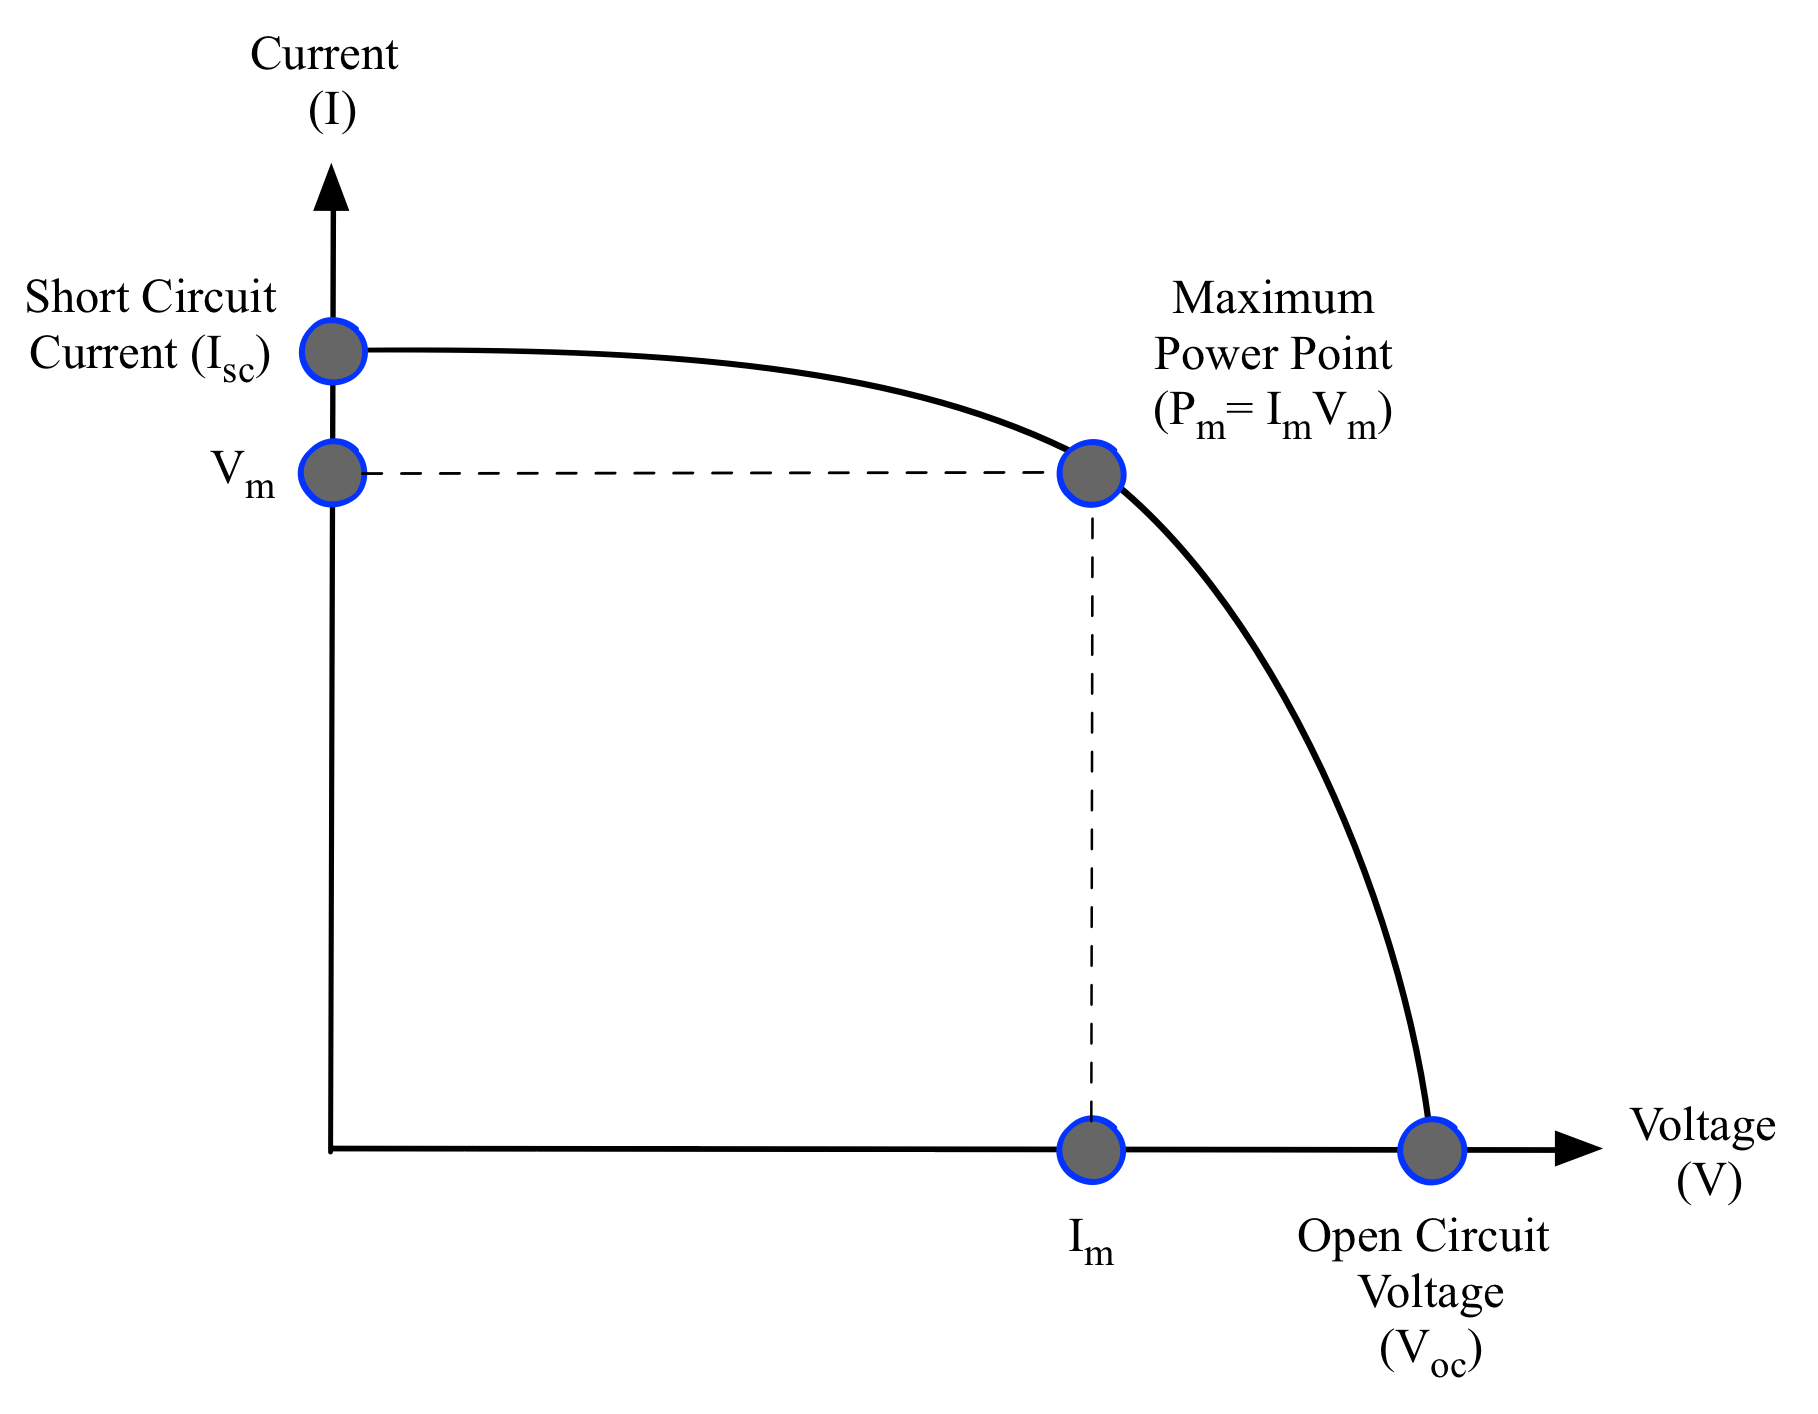
\includegraphics[width=0.65\columnwidth]{figures/ch1/current-voltage.png}
   \caption[Solar cell current-voltage curve]{Schematic of a current-voltage curve for a typical solar cell.}
   \label{current_voltage}
 \end{figure}

The efficiency $\eta$ of the solar cell under an incident light power of $P_\textrm{s}$ is given by
\begin{equation}
    \eta = \frac{P_\textrm{m}}{P_\textrm{s}} = \frac{I_\textrm{m} V_\textrm{m}}{P_\textrm{s}} = \frac{I_\textrm{sc} V_\textrm{oc} \textrm{FF}}{P_\textrm{s}}.
\end{equation}
Thus the three key figures of merit for a solar cell are the $V_\textrm{oc}$, $I_\textrm{sc}$ and FF, and these combine to give the efficiency $\eta$. 
However in all absorber materials there is a trade off between current and voltage; as the bandgap of a material decreases, more photons can be absorbed (higher $I_\textrm{sc}$) but the photogenerated charge carriers have less energy (lower $V_\textrm{oc}$).

%At short circuit, an efficient solar cell does not radiate any light as the excited electrons are extracted before radiative recombination is allowed.
At open circuit, all electrons and holes must recombine in the solar cell. In an efficient PV material the recombination is radiative as this is a thermodynamically unavoidable process via the energy level transitions needed for absorption. Non-radiative recombination, where the energy is dissipated as heat and eventually lost, is avoidable and should be minimised. For a fixed carrier concentration, a higher rate of photon emission corresponds to reduced non-radiative recombination; high radiative efficiency (as measured through e.g. electroluminescence) translates to high open circuit voltage.\autocite{Rau2007}
As a consequence of this reciprocity relation, we can predict the $V_\textrm{oc}$ and $I_\textrm{sc}$ from photoluminescence and photoconductivity studies respectively. This approach has been recently applied to hybrid halide perovskites.\autocite{Braly2018}
% %http://www.nature.com/articles/srep06071 and in Martin Green review for high efficiency PV: http://www.nature.com/nmat/journal/v16/n1/pdf/nmat4676.pdf
% %Also reciprocicty relation Uwe Rau: http://journals.aps.org/prb/abstract/10.1103/PhysRevB.76.085303.
% % Great discussion on this in perovskite review paper on Voc:  10.1002/aenm.201602358.

%plus the other nice paper previous link above I tink.

% %The below outlines how fermi level splitting as measured by PL can be used to predict Voc and JSc and it is applied to perovskties. https://pubs.acs.org/doi/pdf/10.1021/acs.jpclett.8b01152
% %Reciprocity meaning that IPCE and EQE-EL can determine the Voc: http://onlinelibrary.wiley.com/doi/10.1002/aenm.201400812/epdf.
% %ERE is the inverse of EQE and is easier to measure.
% %Can measure El and PL . EL on finished cells bus easier to measure well than PL.
% % $I_EL$ is prop to EQE (extension of reciprocity).
% %Nice description of ERE here: http://science.sciencemag.org/content/351/6280/1401.full
% %PL quantum yield

\subsubsection{The Shockley-Queisser limit}\label{sec:SQlimit}
The principle of detailed balance states that at equilibrium each microscopic process is balanced by its reverse process: for a photovoltaic device operating at open-circuit this means that the rate of photon absorption equals the rate of photon emission. Shockley and Queisser used the principle of detailed balance to calculate the maximum possible efficiency of a photovoltaic device\autocite{Shockley1961} (an alternative derivation is given in Ref. \cite{Nelson2003}). The PV efficiency is dependent upon the direct bandgap $E_g$ of the absorber material and the spectrum of the incident light. Assuming illumination under a standard AM1.5 solar spectrum, the efficiency can be plotted as a function of bandgap. For a single junction solar cell the maximum possible efficiency across is 33\%, which corresponds to an ideal bandgap of $\sim 1.4\,\text{eV}$ (Figure\ \ref{SQlimit}). 

\begin{figure}[h]
\centering
   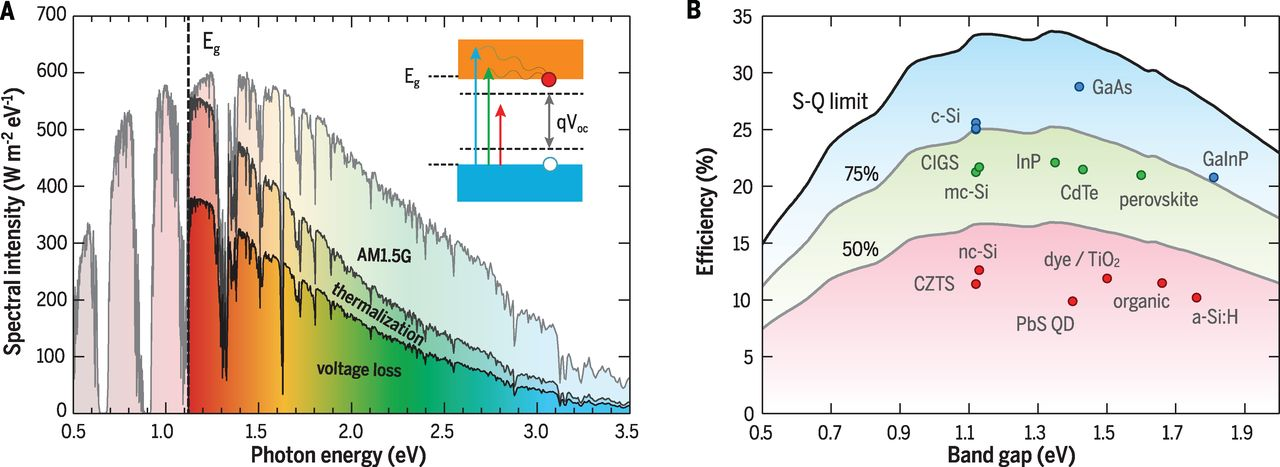
\includegraphics[width=1.0\columnwidth]{figures/ch1/SQlimit.jpg}
   \caption[AM1.5 spectral intensity and Shockley-Queisser efficiency]{(A) The AM1.5 spectrum. Photons below the bandgap are not absorbed, whilst energy is lost from above bandgap photons via carrier thermalisation. (B) The Shockley-Queisser efficiency of a single bandgap solar cell under AM1.5 illumination (thick black line). Also included are the top cell efficiencies for various PV materials. Reprinted with permission from the work of Polman et al.\autocite{Polman2016}}
   \label{SQlimit}
\end{figure}
%https://www.sciencemag.org/help/reprints-and-permissions

The model used to calculate the Shockley-Queisser limit is highly idealised. It assumes that all incident light is absorbed, that every absorbed photon creates an electron-hole pair, and that every electron is extracted to the external circuit. In real materials the absorption coefficient is not a step-function, and excited charge carriers can recombine through non-radiative processes before reaching the circuit. Only three materials have an efficiency above 75\% of the Shockley-Queisser limit: crystalline silicon (c-Si), GaAs and GaInP (Figure\ \ref{SQlimit}). Another metric, the spectroscopic limited maximum efficiency (SLME), accounts for absorption and emission characteristics and reduces the maximum theoretical efficiency.\autocite{Yu2012} For example, the candidate absorber material \ce{CuInS2} has a Shockley-Quiesser maximum efficiency of 33\% and SLME of 29\%.\autocite{Bercx2016} Non-radiative processes which contribute to the efficiency deficit will be discussed further in Section\ \ref{recombination}.

% %%discuss here Zunger SLME - where absorption is accounted for an it is not assumed to be a steo function.
% %% thermodynamic energy losses schematic https://www.nature.com/articles/nmat3263/figures/5

It is possible to exceed the Shockley-Queisser limit by challenging some of the assumptions built into the derivation. For example, the model assumes that once an electron is excited it will thermalise to the band edge, emitting the energy as phonons. This heat energy can no longer do useful work and results in a reduction of the $V_{\text{OC}}$. However `Hot carrier' cells, which extract electrons before they are able to thermalise, were successfully fabricated in 2014 (although it should be noted that they are currently limited to cryogenic temperatures and an incoming spectrum which is intense and monochromatic).\autocite{Hirst2014} 
%Intermediate band solar cells, where an electron recombines with a hole at band edge via a two-step process at a trap state, emitting two photons, have been suggested but have not been realised experimentally.

Another approach is to use tandem solar cells, where several absorber materials are stacked on top of each other. The materials are chosen to have complementary bandgaps, so that more of the solar spectrum can be absorbed with minimal thermalisation losses. GaAs-based four-junction tandem cells have reached an efficiency of 33\% and are used for space applications, though their uptake is limited by the costly wafer bonding method required for fabrication. The constraint of lattice matching -- that the strain at the interfaces must be minimised for device stability -- puts severe limitations on the material combinations which can be used for this approach. 

%Fundamental losses (LC Hirst diagram Prog Photovolt Res. Appl. 19 286 (2010). Carnot and emission is thermodynaics, unavoidable. Boltzmann is entropy (light from all directions, being emitted in one direction) but this can be changes with concentrator (light from all directions) or light only emitted one diection (?). Concentrators can take the form of mirrors (reflecivve) or lenses (refraction). Thermalisation and below Eg can be solved with multi-junctions, IBSC, hot-carriers, multi exciton generation. 


%Other assumptions and technologies which aim to work around this assumption are outlined in Table \ref{beating_SQ} 

% $$ Assumption | Solution | Challenges | Working device $$
% Single bandgap | Tandem solar cells | 
% Electrons will thermalise before being extracted to external circuit | Hot carrier solar cells | GaAs / quantum wells?
% Each photon generates a single electron | Intermediate band solar cells
% Boltzmann losses | concentrator PV | %


% schematic here

%Beating the SQ limit takes us from very basic physics to engineering.
%The SQ limit can be overcome by using solar concentrators (which is equivalent to not letting light escape) or by having an intermediate bandgap solar cell (see Jarv paper)
%- Concentrators: no boltzmann losses.
%- ALCHEMI project.
%- hot carrier solar cells. GaAs, Dimmock, 2014, progress in PV. cryogenic. intense, monochromic light. high risk / high reward.
%- It’s all about tandem solar cells (GaAs) for high value, niche market PV. The challenge is lattice matching. They have a 4J 33\% GaAs for space application. Fabricated using MBE/MOVPE (more expensive).
%- Ratchet route – intermediate band solar cell – requires that the intermediate band does not become a place for recombination which can happen when introduced as a defect band as is usually done (can’t be single defect state: wont be able to build up considerable charge)
%Hot carrier has potential to make huge gains. But incredible tight material specification. Needs to be incredibly physically thin.
%Multijunction cells are great. Boltzmann loss increases but there are gains re: thermalisation and bandgap losses (louis hirst paper). Problem is lattice matching the MJ cells. Wafer bonding allows different attice parameters but is costly: there is always a trade.
%Spectral splitting. Interstitial light trapping.
%- New architectures: tandem etc. 33\% reached:https://www.nature.com/articles/s41560-018-0125-0
%- Concentrated PV is used to offset the cost of
%- multijunctuion PV.
%- Lattice matching in PV is problematic esp. over a range of temperatures. MOVCD iii-v on Si. Quantasol

%for polycrystalline:. Bryan huey - nanoscale tomography of photocarrier transport in operating CdTe solar cells. The AFM technique allows to map the PV properties (I-V, Isc, Voc) with high spatial resolution so we see that the Isc and Voc couple to the microstructure.

%Following the work of Hirst et al., the 
%- ned edkins dauke publications about different types of loss. Loise Hirst, progress in PV. Lovely schematic from 2011: Louise hirst: fundamental loss in solar cells, progress in PV. Carnot and emission is thermodynaics, unavoidable. Boltzmann is entropy (light from all directions, being emitted in one direction) but this can be changes with concentrator (light from all directions) or light only emitted one diection (?). Concentrators can take the form of mirrors (reflecivve) or lenses (refraction). Thermalisation and below Eg can be solved with multi-junctions, IBSC, hot-carriers, multi exciton generation. 
%- this is related to the unavoidable thermodynamic losses due to entropy (see Ross). PLQY can be used to give us the quasi fermi level splitting.
%- about thermodynamic losses: good review: https://journals.aps.org/prb/abstract/10.1103/PhysRevB.90.035211

\subsection{Carrier recombination} \label{recombination}
Electron-hole recombination competes with charge extraction to the external circuit, and as such it is a well examined process. Three pathways for electron-hole recombination are outlined in Figure\ \ref{recombination_processes}. During radiative recombination the electron directly recombines with a hole to produce a photon and, in the case of indirect recombination, phonons. This recombination channel is unavoidable in PV devices as the same channel is used for light absorption. The second pathway, Shockley-Reed-Hall (SRH) recombination, is a two step process mediated via a defect trap state. In PV devices this pathway should be minimised as the kinetic energy of the electron and hole is transformed to vibrational energy (phonons) and cannot be used for useful work. The third pathway, Auger recombination, is also a non-radiative process. Here the electron directly recombines with a hole, and the resulting energy and momentum is transferred to another conduction band electron.
% %4.4x10^18 is auger recombination in MAPI - see Tom hopper work when it comes out.

\begin{figure}[h]
 \centering
   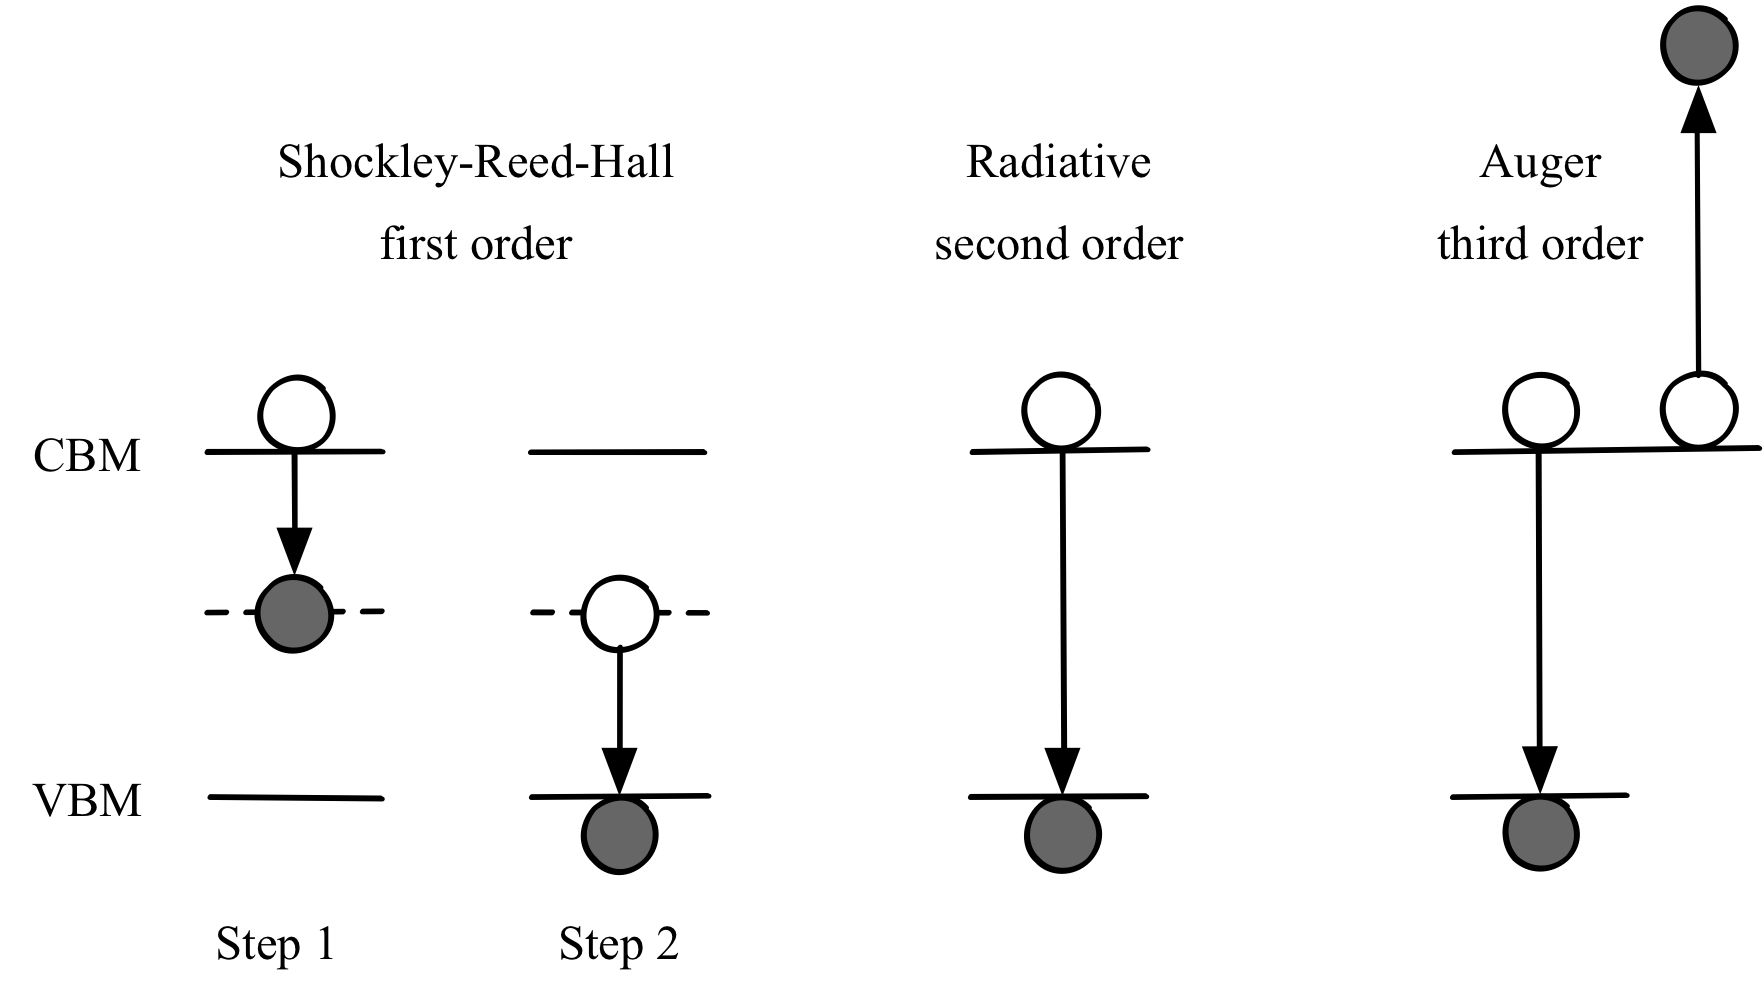
\includegraphics[width=0.65\columnwidth]{figures/ch1/recombination.png}
   \caption[Electron-hole recombination pathways]{A schematic of the three possible electron-hole recombination pathways. In each case, an electron at the conduction band minimum combines with a hole at the valence band maximum. Empty (filled) circles correspond to the electron before (after) each transition. First-, second- and third-order processes correspond to one, two and three particle processes respectively.}
   \label{recombination_processes}
 \end{figure}

Radiative recombination and Auger recombination are unavoidable processes intrinsic to the material, whereas SRH recombination is an avoidable process that can be controlled through defect engineering. The SRH recombination rate is given by
\begin{equation}
U_\textrm{SRH} = \frac{np-n_\textrm{i}^2}{\tau_\textrm{n,SRH}(p+p_\textrm{t})+\tau_\textrm{p,SRH}(n+n_\textrm{t})},
\end{equation}
where $n$ ($p$) is the density of electrons (holes), $n_i$ is the intrinsic carrier density and $n_\mathrm{t}$ ($p_\mathrm{t}$) is the value of the electron (hole) density when the electron Fermi level is equal to the trap level $E_\mathrm{t}$: 
\begin{align}
n_\mathrm{t} &= n_\mathrm{i}e^{\frac{(E_\mathrm{t}-E_\mathrm{c})}{k_\mathrm{B}T}} \\
n_\mathrm{p} &= n_\mathrm{i}e^{\frac{(E_\mathrm{v}-E_\mathrm{t})}{k_\mathrm{B}T}},
\end{align}
where $E_\mathrm{c}$ and $E_\mathrm{v}$ are the energies of the CBM and VBM respectively. The recombination rate has a maximum when the rates of hole capture and electron capture are comparable. This happens when the trap level is in the middle of the bandgap, and $n_\mathrm{t} = p_\mathrm{t}$. % note here that deep state not needed: czts : https://pubs.acs.org/doi/pdf/10.1021/acsenergylett.7b01313

$\tau_\textrm{n,SRH}$ ($\tau_\textrm{p,SRH}$) is the electron (hole) lifetime. For a trap density $N_\mathrm{t}$, mean thermal electron (hole) velocity $v_\mathrm{n
}$ ($v_\mathrm{p}$) and electron (hole) capture cross section $\sigma_\mathrm{n}$ ($\sigma_p$), the lifetimes can be approximated as 
\begin{align}
\tau_\textrm{n,SRH} &= \frac{1}{v_\mathrm{n}\sigma_\mathrm{n}N_\mathrm{t}} \\
\tau_\textrm{p,SRH} &= \frac{1}{v_\mathrm{p}\sigma_\mathrm{p}N_\mathrm{t}}.
\end{align}
The standard approach for calculating the trap density from first principles is give in Chapter\ \ref{ch:3-methods}, and a method for calculating the capture cross section is outlined in the Chapter\ \ref{ch:6-defects}.

\subsubsection{Experimental measurements of recombination rates} \label{exprecombo}

Carrier lifetimes and recombination rates are difficult to measure experimentally as ultra fast optical and electronic sensors are needed to capture transient behaviour, and this must be done in conditions relavant to photovoltaic performance. Time resolved photoluminscence (TRPL) and photoconductivity measurements are used to infer the recombination rates for each recombination pathway.
Each pathway scales differently with carrier concentration, as specified by the following rate equation:
\begin{equation}
\frac{d n}{d t} = G -k_1n -k_2n^2 -k_3n^3 
\end{equation}
where $G$ is the rate of electron-hole generation, $k_1$ is the rate constant for SRH recombination, $k_2$ is the rate constant for radiative recombination and $k_3$ is the rate constant for Auger recombination. SRH recombination via a trap state is a one particle process that scales linearly with the carrier concentration. Radiative recombination is a two particle process that depends on the electron density and hole density, so scales quadratically with carrier concentration. Auger recombination requires three particles and scales cubically.
TRPL uses short laser pulses to excite excess electrons and holes which then decay via recombination or carrier extraction at an interface. Exponential curves are fitted to the TRPL signal at different laser fluences to extract carrier lifetimes. In general, for solar cells operating under 1.5AM illumination, second order SRH recombination is the dominant recombination mechanism.
% 
% https://www-herz.physics.ox.ac.uk/publications/Herz16a.pdf
% https://aip.scitation.org/doi/10.1063/1.4891595
% https://www.nanoge.org/proceedings/ABXPV/58c15c889c168f501d8b9aa2


 \subsection{Design principles for absorber materials}
 
Solid state physics and computational chemistry can connect microscopic material processes to macroscopic observables. The tools of each field have been applied to a range of inorganic and organic materials, and have successfully explained the observed properties of existing materials.
There is also a more recent approach to materials science called ``inverse design''. This is where the desired functionality of a new material is stated first, and computational tools are used to predict which materials will exhibit such features.\autocite{Zunger2018}
The hope is that this approach will improve upon discovery by trial and error, and accelerate the design of new materials.
%Previous technologically important material properties were discovered by trial and error (e.g. superconductivity, giant magneto resistivity);

High-throughput computational screening is a brute force approach to inverse design. Here, an automated procedure calculates a set of properties across a large number of atomic structures. This approach has been used to identify battery electrolytes,\autocite{Qu2015} organic photovoltaic materials\autocite{Hachmann2011} and materials for carbon capture and storage,\autocite{Dunstan2016} amongst others. 
Materials screening criteria must be defined so that successful materials are identified and selected for further study. Some criteria are easy to identify - for example the thermodynamic stability, which ensures that the material is synthesisable. This criteria can be expanded to include the features found in existing successful materials. For example, hybrid halide perovskites are defect tolerant - they contain a low concentration of defects which are detrimental to opto electronic performance. The electronic parameters which underpin the defect tolerance of hybrid halide perovskites have been identified so that they may be used to screen for new defect-tolerant materials.\autocite{Brandt2015} 
% https://pubs.rsc.org/en/content/articlelanding/2016/EE/C5EE03253A#!divAbstract
% https://pubs.acs.org/doi/10.1021/jz200866s
% https://perssongroup.lbl.gov/papers/compmatsci2015-electrolytegenome.pdf

With the concept of inverse design in mind, items for a successful PV material ``shopping list'' are listed below. The final three items (toughness, elemental abundance, elemental non-toxicity) are not necessary for successful devices in the lab, but would promote commercialisation of the technology.


\textbf{Thermodynamic stability}

The material should be thermodynamically stable with regard to competing phases so that it does not degrade over years of operation. The binary compound CdTe was the first thin film PV material to be commercialised and, similar to GaAs, it has no competing phases. Quaternary chalcogenide compounds such as \ce{CISSe} and CZTS have many more competing phases to consider and the chemical potentials during synthesis must be very finely tuned for stability, which hinders their development.
% Cu3Bi5S3 chalcogenide (major group). 0.1\% efficiency. Probelm: other phases. Keep it cimple: Sb2S3/Sb2Se3 - 5.5% with 3o papers/
%The same thing that makes a material have a good bandgap is that which makes it degrade (something about the bonding strenght??)


\textbf{Optimum bandgap}

Ultimately, it is the spectrum of the sun and features of our atmosphere (light scattering and absorption) that dictates the design of solar cells; we must optimise our solar technology to take advantage of the spectrum that is particular to our planet. The Shockley-Queisser limit, discussed in subsection\ \ref{sec:SQlimit}, gives an optimum bandgap of \SI{1.4}{\electronvolt}.\autocite{Ruhle2016}
Atomic disorder or point defects can reduce the material band gap. Quaternaries with elemental species of a comparable atomic radii are more likely to exhibit atomic disorder -- for example in CZTS this leads to a bandgap reduction of \SI{30}{meV}.\autocite{Rey2018}


\textbf{Strong light absorption}

The absorption coefficient specifies how much light of a particular wavelength is absorbed by a material. Different semiconductor materials have different absorption coefficients; those with a higher absorption coefficient will more readily absorb light. Silicon is an indirect bandgap material that requires phonon-assisted absorption. As a result, crystalline silicon absorbs 92\% of light in a thickness of  \SI{200}{\micro\metre}, whilst CdTe can absorbe the same amount in a thickness of \SI{1}{\micro\metre}.\autocite{Poortmans2006}
%As a result of relativistic spin-orbit coupling, the hybrid halide perovskite MAPI is also an indirect bandgap material. However, as spin splitting of the conduction band edge is small () and the density of states at the valence band edge is large, this has a negligible influence on light absorption in the material.\autocite{Azarhoosh2016}


\textbf{Low exciton binding energy}

After light absorption, a bound electron-hole pair (exciton) is created. The electron and hole must disassociate so that they can travel to their respective contacts. Here, the dielectric response is key, as this determines how readily a material will screen electrostatic perturbations. Organic solar cell materials are limited by low dielectric constants ($\epsilon_0 \approx 3-4$) that lead to large exciton binding strengths.\autocite{Brebels2017} In inorganic or hybrid materials the dielectric constants are higher ($\epsilon_0=10.4$ for CdTe,\autocite{Madelung2004} whilst values vary from $\epsilon_0=16.6$ to $\epsilon_0=28.5$ for MAPI\autocite{Wilson2019}).
% dielectric constant - effective mass theory
% polar domains for charge separation


\textbf{High carrier mobility}

Some materials may have suitable optical properties but are unable to transport the photogenerated charge efficiently to the contact layers. Carrier mobility quantifies how quickly an electron or hole can move through a material when pulled by an electric charge. 
Light carrier effective masses (high band dispersions) correspond to higher mobilities. However light effective masses are not sufficient in themselves as there are various scattering channels to consider: lattice scattering, carrier-carrier scattering and defect scattering. The most significant scattering mechanisms in a PV material are lattice scattering and ionized defect scattering.
A high dielectric constant is beneficial to carrier mobility as the rate of ionized defect scattering is proportional to $\frac{1}{\epsilon^2}$. The composition of the material is also important -- for example, vacancies in gallium nitride (Ga$^{3+}$N$^{3-}$) carry a larger charge and have a larger scattering cross section than vacancies in MAPI (\ce{CH_3NH_3}$^{1+}$Pb$^{2+}$I$^{1+}_3$).


\textbf{Long carrier lifetime}

Carrier lifetime has already been discussed in the context of electron-hole recombination in Section\ \ref{recombination}. Whereas the concentration of defects is important for carrier mobility, here it is the energy of defect states with respect to the valence and conduction band which is important. This is discussed in Chapter \ref{ch:6-defects}. In summary, the key is to minimise non-radiative recombination via deep level defect states (also known as ``killer defects''). Carrier diffusion length, another important figure of merit with regard to carrier transport, is proportional to the product of carrier mobility and lifetime.


\textbf{Compatibility}

For efficient charge extraction, the PV absorber layer must be compatible with suitable contact and/or buffer layers. Firstly, the energy levels of the interfacing materials must align so that there is an electrical potential gradient to extract the charge, without significant loss of $V_\textrm{OC}$. For example, band mis-alignments are reported to be the source of poor photovoltaic efficiencies in the candidate absorober materials \ce{BiSI} and \ce{BiSeI}.\autocite{Ganose2016} Secondly, lattice mismatch at the interface should be avoided as this can lead to deep point defects that provide sites for non-radiative recombination and, in the case of more severe strain, an incoherent interface with many defect sites and weak chemical bonding. Computational screening procedures can be used to identify potential electronically and structurally matched contact layers and this has been recently applied to the hybrid halide perovskites.\autocite{Butler2016}
%more examples?
% http://science.sciencemag.org/content/sci/352/6283/aad4424.full.pdf “Photovoltaic materials: Present efficiencies and future challenges”


\textbf{Toughness}
This is disc
Silicon is a brittle material; the majority of Si material in a solar cell is used as a mechanical carrier to prevent crack propagation, and glass must be used as a protective layer. The resulting cell is often too heavy to be installed on structures which are made from wood or sheet metal. In addition, the bulk of system costs are higher for heavier cells. Organic photovoltaics, and to some extent perovskites, are tougher and can be made using roll-to-roll print processes onto a flexible substrate.


\textbf{Elemental abundance}

The power generated from PV installations must exceed \SI{1}{TW} to make a real impact on global carbon emissions.\autocite{Battersby2019} To meet this demand, PV materials must be made from abundant elements that are in ready supply at reasonable cost. To quantify this criteria, the Herfindahl–Hirschman index (HHI), which is used in economics as a measure of market concentration, can be applied to elements. The HHI indicates that Si is abundant but that production is highly concentrated in a few countries. Elements common to the third generation of materials---Cu, Zn, S, Se, Sn---are less abundant but their production is more highly distributed across the globe.\autocite{Gaultois2013}


\textbf{Elemental non-toxicity} 

Finally, toxic elements may hinder the succesful commercialisation of future PV technologies. The problem is not insurmountable; cadmium telluride is toxic if ingested but is a commercial solar cell material. Encapsulation and recycling can reduce any risk, but add another level of complexity to the development of new solar technologies.

\section{Summary}

% need to point out that the highest efficiencies are from single crystal silicon and GaAs 26-29 mark. Lower cost polycrystalline in 20-23 mark. http://science.sciencemag.org/content/sci/352/6283/aad4424.full.pdf
To reduce the rate of climate change we must decrease our reliance on fossil fuels, and increasing the proportion of photovoltaic energy is one way to achieve this. This may only be politically feasible if the costs associated with PV energy can continue to exponentially decrease. As the well-established silicon technologies are limited by high capital expenditures, there is an incentive to develop new low-cost, high-efficiency and reliable technologies. Flexible thin-film architectures also allow for expansion into the new market of building integrated photovoltaics. Currently no material has met these requirements,\autocite{Zakutayev2017} although promising performance from emerging technologies such as the hybrid halide perovskites motivates further research.
% - start with what needed in general then what needed material properties wise to deliver this.
% - defects run throughout this chapter:
% - Defects can be fatal and vital : (good chapter quote?): Defects in Semiconductors: Some Fatal, Some Vital Hans J. Queisser* and Eugene E. Haller 
% - Ability to accelerate the design of PV materials through computation. Growth in computational tools (web of science keyword search), accesibility to non-specialists

% - light management vs carrier management. engineering vs basic science.

% Learn from the Si community: passivate the grain boundaries, specific and controlled doping, improve material quality, bandgap grading.
% Seen a 
% Wish list of properties.

% Key themes in this work: SRH.

\section{Thesis outline}

Organic-inorganic halide perovskites present a number of challenges for first-principles atomistic materials modelling. These `plastic crystals' feature dynamic processes across multiple length-scales and time-scales, which include mixed ionic-electronic transport, highly anharmonic lattice dynamics and strong relativistic (spin-orbit coupling) effects on the electronic band structure.
These issues, which affect the operation of solar cells, are outlined in a review of the literature. 
This is followed by a brief introduction to the theory that underlies almost all of the work in this thesis - Density Functional Theory (DFT). 
To model an imperfect material (one with crystal defects), or a material at finite temperature, there are a series of post-processing steps that follow the DFT calculation. These are also outlined in Chapter Three.

Chapters Four to Six contain the thesis results. Each results chapter contains any additional theory, where required, and calculation steps. Bulk transport and optical properties of the perfect material are calculated using Effective Mass Theory (EMT) in Chapter Three. 
EMT often assumes a parabolic electronic band dispersion, however in this chapter non-parabolic distortions are considered.
Temperature effects are introduced in Chapter Four. 
At room temperature the inorganic octahedral \ce{PbI3} units tilt back and forth, and the coupling strength between this tilting and the electronic sub-sytem is quantified.
Finally, point defects are introduced to our model in Chapter Six. Point defects can be benign or harmful to device performance, depending upon the properties of the defect. This chapter focuses on the iodine interstitial point defect and gives the rate of charge trapping at this defect site.
% check that it actually does this!



\begin{savequote}[8cm]
It's simple mathematics.
  \qauthor{--- Mos Def, \textit{Mathematics}}
\end{savequote}

\chapter{\label{ch:2-litreview}Simulation of hybrid halide perovskites}

The text and figures in this chapter are adapted from \href{https://doi.org/10.1063/1.4984964}{Whalley, L. D., Frost, J. M., Jung, Y. -K. and Walsh, A. (2017). Perspective: Theory and simulation of hybrid halide perovskites. \textit{The Journal of Chemical Physics}, 146(22), p.220901.} © 2017 CC-BY

\section{Introduction}

In this chapter I address recent progress and current challenges in the theory and simulation of hybrid perovskites. 
Particular attention is paid to predicting properties that assess the photovoltaic potential of a material. 
Factors to consider include: light absorption, charge transport, absolute band energies, defect physics and chemical stability. 

The perovskite mineral, \ce{CaTiO3}, is the archetype for the structure of many functional materials.\autocite{Schaak2002}
Metal halide perovskites have been studied for their semiconducting properties since the 1950s\autocite{Moller1958}; 
yet only recently have organic-inorganic perovskites such as \ce{CH3NH3PbI3} (MAPI) been applied to solar energy conversion, showing remarkably strong photovoltaic action for a solution processed material.\autocite{Kojima2009}
The field has progressed rapidly in the past eight years, with the increase in power conversion efficiency supported by over three thousand research publications.\autocite{Stranks2015b,Saparov2016b,Park2016,Walsh2016,Wallace2017}
Other potential application areas of these materials include 
thermoelectrics,\autocite{He2014,Mettan2015}
light-emitting diodes,\autocite{Protesescu2015,Stranks2015b}
and
solid-state memory.\autocite{Yoo2015a,Liu2017}

These materials combine a complex crystal structure, modulated by static and dynamic disorder, with an electronic structure requiring methods beyond density functional theory to treat many-body and relativistic effects. 
As such, the halide perovskites represent a challenge to predictive materials modelling. 
% https://www.youtube.com/watch?v=fAnP2ck-7o4

\begin{figure*}
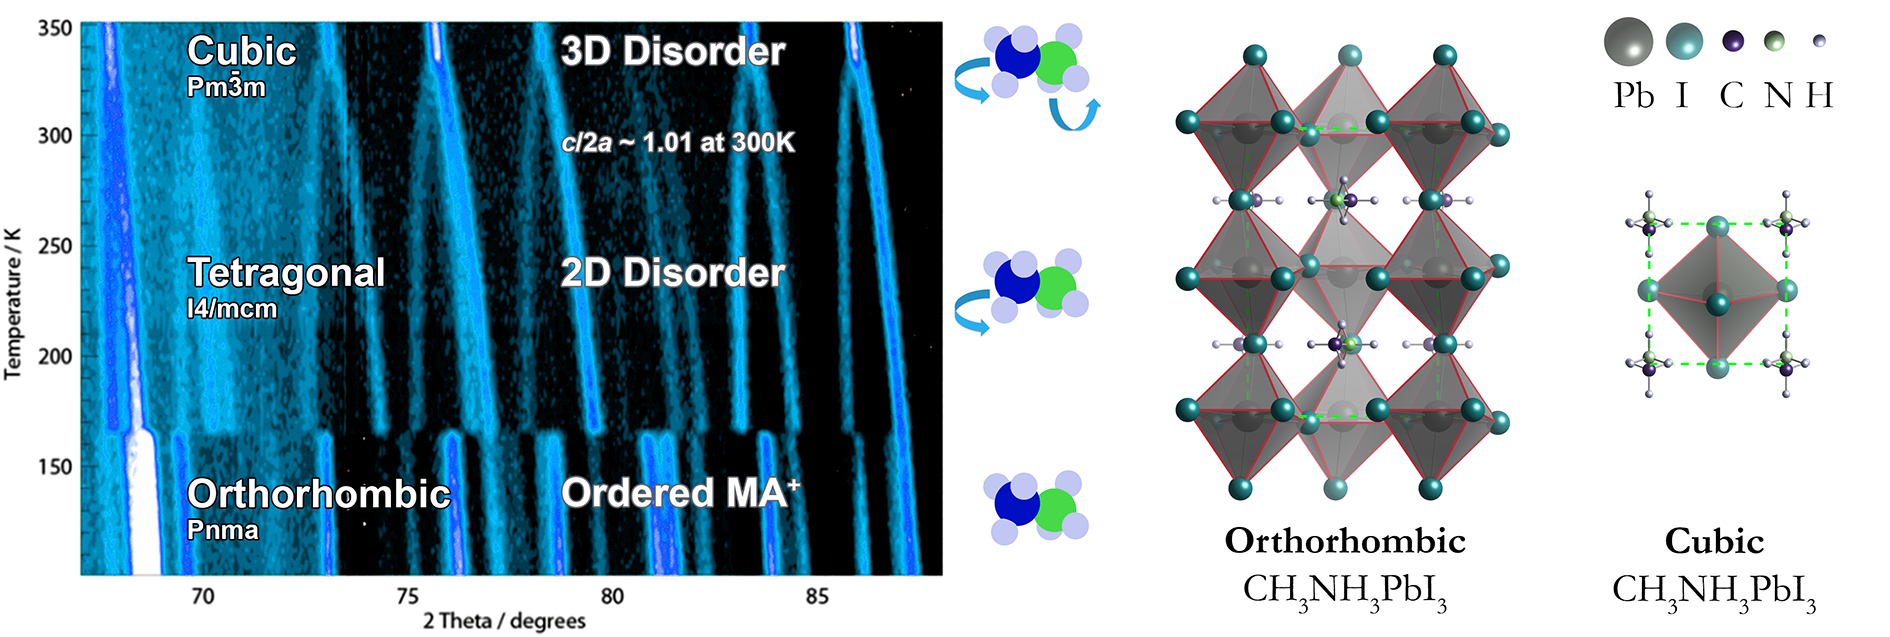
\includegraphics[width=1.0\columnwidth]{./figures/ch2/f1.png}
\caption[\ce{CH3NH3PbI3} powder neutron diffraction pattern and crystallographic unit cells]{
The high-resolution powder neutron diffraction pattern of the hybrid halide perovskite \ce{CH3NH3PbI3} is shown in the left panel (adapted with permission from Ref. \autocite{Frost2016a} based on data in Ref. \autocite{Weller2015}), which illustrates the low and high temperature phase transitions. While an ordered \ce{CH3NH3+} sub-lattice is expected in the orthorhombic phase, orientation disorder increases with temperature. 
The crystallographic unit cells of the pseudo-cubic and orthorhombic perovskite phases are shown in the right panel (adapted with permission from Ref. \autocite{Brivio2015a}). The associated structure files can be accessed from \url{https://github.com/WMD-group/hybrid-perovskites}. Figure prepared by Aron Walsh.
}
\label{fig1}
\end{figure*}

\section{Crystal structures and lattice dynamics} 

\subsection{Phase diversity}
Hybrid perovskites of the type \ce{ABX3} form a crystal structure with an organic A site cation contained in an inorganic \ce{BX3} framework of corner sharing octahedra. 
Halide substitution on the X site (X = \ce{Cl-}, \ce{Br-}, \ce{I-}), metal substitutions on the B site (B = \ce{Pb^2+}, \ce{Sn^2+}), and cation substitution on the A site (A = \ce{CH3NH3+}, \ce{HC(NH2)2+}, \ce{Cs+}, \ce{Rb+}) lead to various chemical and physical properties.\autocite{Mitzi2001,Mitzi2004a}
In addition to isoelectronic substitutions (e.g. replacing \ce{Pb^2+} by \ce{Sn^2+}), it is possible to perform pairwise substitutions to form double perovskites (e.g. replacing \ce{2Pb^2+} by \ce{Bi^3+} and \ce{Ag^+}).\autocite{Savory2016,Volonakis2016}

In the first report of MAPI by Weber in 1978, the crystal structure was assigned as cubic perovskite (space group $Pm\bar{3}m$).\autocite{Weber1978,Weber1978a}
The anionic \ce{PbI3-} network is charge balanced by the  \ce{CH3NH3+} molecular cation.
The symmetry of \ce{CH3NH3+}  ($C_{3v}$) is incompatible with the space group symmetry ($O_h$) unless orientation disorder (static or dynamic) is present.
The crystal structure solved from X-ray or neutron diffraction data usually spread the molecules over a number of orientations with partial occupancy of the associated lattice sites.
A common feature of perovskites is the existence of phase changes during heating (typically from lower to higher symmetry) as shown in Figure \ref{fig1}. 
In hybrid halides containing methylammonium, these are orthorhombic ($Pnma$), tetragonal ($I4/mcm$) and cubic ($Pm\bar{3}m$) phases.\autocite{Weller2015} 
%
For MAPI the $Pnma$ to $I4/mcm$ phase transition is first-order with an associated discontinuity in physical properties, while the $I4/mcm$ to $Pm\bar{3}m$ phase transition is second-order with a continuous evolution of the structure and properties.\autocite{Onoda-Yamamuro1990,Weller2015}

The phase transitions are linked to a change in the tilting pattern of the inorganic octahedral cages, and order-disorder transitions of the molecular sub-lattice.\autocite{Onoda-Yamamuro1990,Yamamuro1992a,Onoda-yamamuro1992}
X-ray diffraction (XRD) measurements upon cooling (heating) suggest the incursion of tetragonal in orthorhombic phases (and vice versa),\autocite{Hutter2016a}
which is common for first-order solid-state phase transitions. 

Similar phase behaviour tends to be seen for other compositions; however, the transition temperatures vary.
In MAPI the orthorhombic to tetragonal transition temperature is $162$ K, becoming cubic by around $328$ K,
while \ce{CH3NH3PbBr3} is cubic above $237$ K.\autocite{Poglitsch1987c} 
%

\begin{figure*}
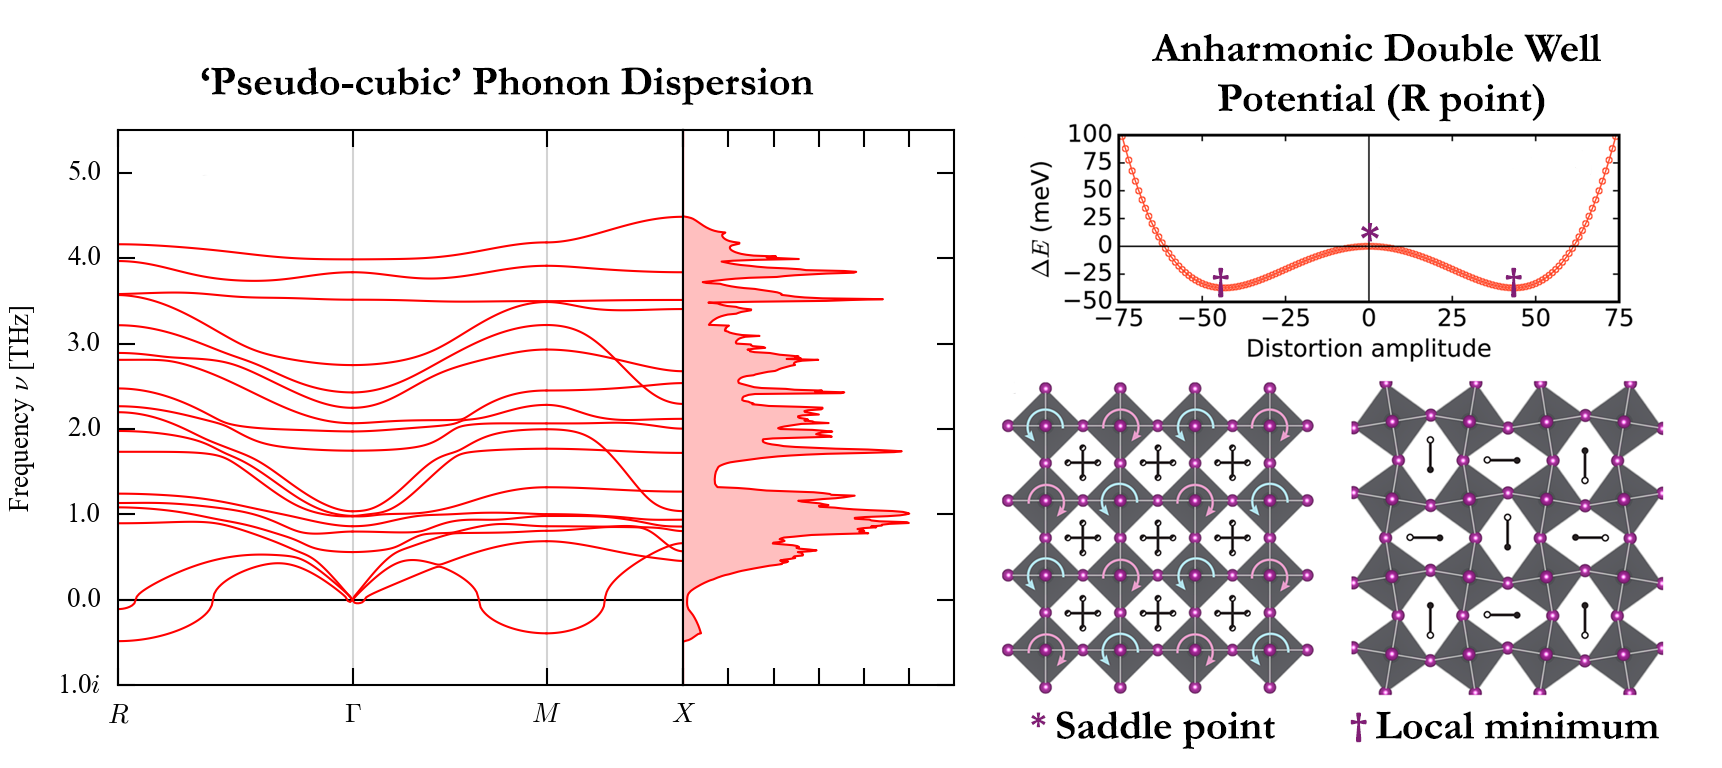
\includegraphics[width=1.0\columnwidth]{./figures/ch2/f2.png}
\caption[\ce{CH3NH3PbI3} phonon dispersion and double-well potential energy surface]{
    (Left) The harmonic phonon dispersion for \ce{CH3NH3PbI3} from a `pseudo-cubic' structure. 
    The imaginary frequencies of acoustic modes at the $M$ ($q=\frac{1}{2},\frac{1}{2},0$) and $R$ ($q = \frac{1}{2}, \frac{1}{2}, \frac{1}{2}$) Brillouin zone boundary correspond to an instability expressible in a supercell as alternate tilting of the octahedra.
    (Right) Following the imaginary acoustic mode at the $R$ Brillouin zone boundary in a $2\times2\times2$ supercell expansion shows a double-well potential in the DFT internal energy. 
    The saddle point corresponds to a $1\times1\times1$ cubic structure, whilst the two local minima correspond to a distorted structure of lower symmetry. 
The energy barrier is small enough to allow both minima can be accessed at room temperature, so the system is expected to exhibit dynamic rather than static disorder. 
Similar behaviour is found at the $M$ point. 
Figure adapted by Aron Walsh with permission from Refs. \cite{Whalley2016} and \cite{Beecher2016a}.
The underlying phonon data is available from \url{https://github.com/WMD-group/Phonons}.
}
\label{fig2}
\end{figure*}

\subsection{Local and average crystal environment} \label{localaverage}

The first electronic structure calculation of hybrid halide perovskites was by Chang, Park and Matsuishi in 2004, \autocite{Chang2004}
in the local density approximation (LDA) of density functional theory (DFT).
They modelled a static structure where the \ce{CH3NH3+} molecule was aligned along $\langle100\rangle$ (towards the face of the corner-sharing \ce{PbI3-} framework), but found that the barrier for rotation to $\langle111\rangle$ was less than $10$ meV. 
This small barrier for cation rotation gave credence to a prior model that the molecular sub-lattice was dynamically disordered.\autocite{Poglitsch1987c}
Similar barriers were later found within the generalised gradient approximation (GGA) of DFT.\autocite{Brivio2013} 
%JMF: Bit of a 'me too' citation? Anything extra to add? - AW: Unfortunately not, and we had missed the ealier paper at that time :(

\emph{Ab initio} molecular dynamics (MD), neutron scattering\autocite{Leguy2015b,Chen2015s} and time-resolved infra-red\autocite{Bakulin2015a} data all indicate a 1--10 picosecond reorientation process at room temperature.
As a result of anharmonic molecular rotation, and large-scale dynamic distortions along soft 
vibrational modes, the local structure can deviate considerably from that sampled by diffraction techniques, which do not probe local disorder that preserves long-range order on average.

In spite of the larger cation, FAPI appears to possess a similar timescale of rotation to MAPI\autocite{Weller2015b}. 
A lighter halide (and therefore smaller cage) results in faster rotation, in spite of the greater steric hindrance.\autocite{selig2017organic}
Together, these data suggest that the molecular rotation is a function of the local inorganic cage tilting, where the relatively insignificant mass of the organic cation follows the pocket distortion. 

The spontaneous distortions can also be observed in the vibrational spectra.
The calculated harmonic phonon dispersion for MAPI in the cubic phase is presented in Figure \ref{fig2}.
The acoustic modes soften as they approach the $M$ ($q = \frac{1}{2}, \frac{1}{2}, 0$) and $R$ ($q = \frac{1}{2}, \frac{1}{2}, \frac{1}{2}$) Brillouin zone boundaries. 
This zone boundary instability can only be realised in an even supercell expansion, where it corresponds to anti-phase tilting between successive unit cells.
This behaviour is characteristic of the perovskite structure,\autocite{Yang2017} and can be described by the Glazer tilt notation.\autocite{Glazer1972,Woodward1997} 
%and has been recently identified as common to all inorganic halide perovskites. %cite ruoxi. 

Within the frozen-phonon approximation the potential energy surface can be traced along the soft acoustic $M$ and $R$ modes. 
In both cases this results in a double well with an energy barrier $\sim k_\mathrm{B}T$ at the saddle point;\autocite{Whalley2016}   
at room temperature the structure is dynamically disordered, with continuous tilting.
Indeed, MD simulations show continuous tilting of MAPI and FAPI at room temperature.\autocite{Frost2014,Quarti2015a,Weller2015b}
%
As temperature decreases, the structural instability condenses via the $R$ point (with an energy barrier of 37 meV) into the lower symmetry tetragonal phase. 
This is followed by condensation of the $M$ point (with an energy barrier of 19 meV) to the orthorhombic phase.\autocite{Whalley2016}

In the static picture -- as in the case of an electronic band structure calculated for a single ionic snapshot -- the organic cation plays no direct role in optoelectronic properties of the material as the molecular electronic levels lie below that of the inorganic framework.
Once motion is considered, the electrostatic and steric interaction between the organic molecule and inorganic framework couples tilting and distortion of the octahedra to the organic cation motion.
These tilts and distortions vary the orbital overlap between states, perturbing the band-structure and band-gap.\autocite{Mosconi2014,Quarti2015a,Whalley2016,Saidi2016}
The electronic structure thus becomes sensitive to temperature, which will be discussed further in Section \ref{ch2epcoupling} and Chapter \ref{ch:5-epcoupling}.

\subsection{Thermodynamic and kinetic stability}

\textit{Ab initio} thermodynamics has emerged as a powerful tool in materials modelling, with the ability to assess the stability of new materials and place them on equilibrium phase diagrams even before experimental data is available. \autocite{Reuter2003,Kim2012,Jackson2015a}
The total energy from DFT calculations approximates the internal energy of the system. 
By including lattice vibration (phonon) and thermal expansion contributions, the Gibbs free energy 
and other thermodynamic derivatives can be evaluated.\autocite{Stoffel2010}
In the context of photovoltaic materials, this has been applied to \ce{Cu2ZnSnS4} 
and used to identify the processing window where a single-phase compound can be grown in equilibrium.\autocite{Jackson2014}

An issue with hybrid perovskites and other metal-organic frameworks is that the calculated heat of formation is close to zero.
The decomposition reaction 
\begin{equation}
\ce{CH3NH3PbI3} \rightarrow \ce{CH3NH3I} + \ce{PbI2}
\end{equation}
has been predicted to be exothermic.
%
Subsequent calorimetric experiments have supported the prediction that hybrid lead halide perovskites are metastable.\autocite{Nagabhushana2016}
%
It is likely that these materials are only formed due to entropic (configurational, vibrational and rotational) contributions
to the free energy.

\begin{figure*} \label{f3}
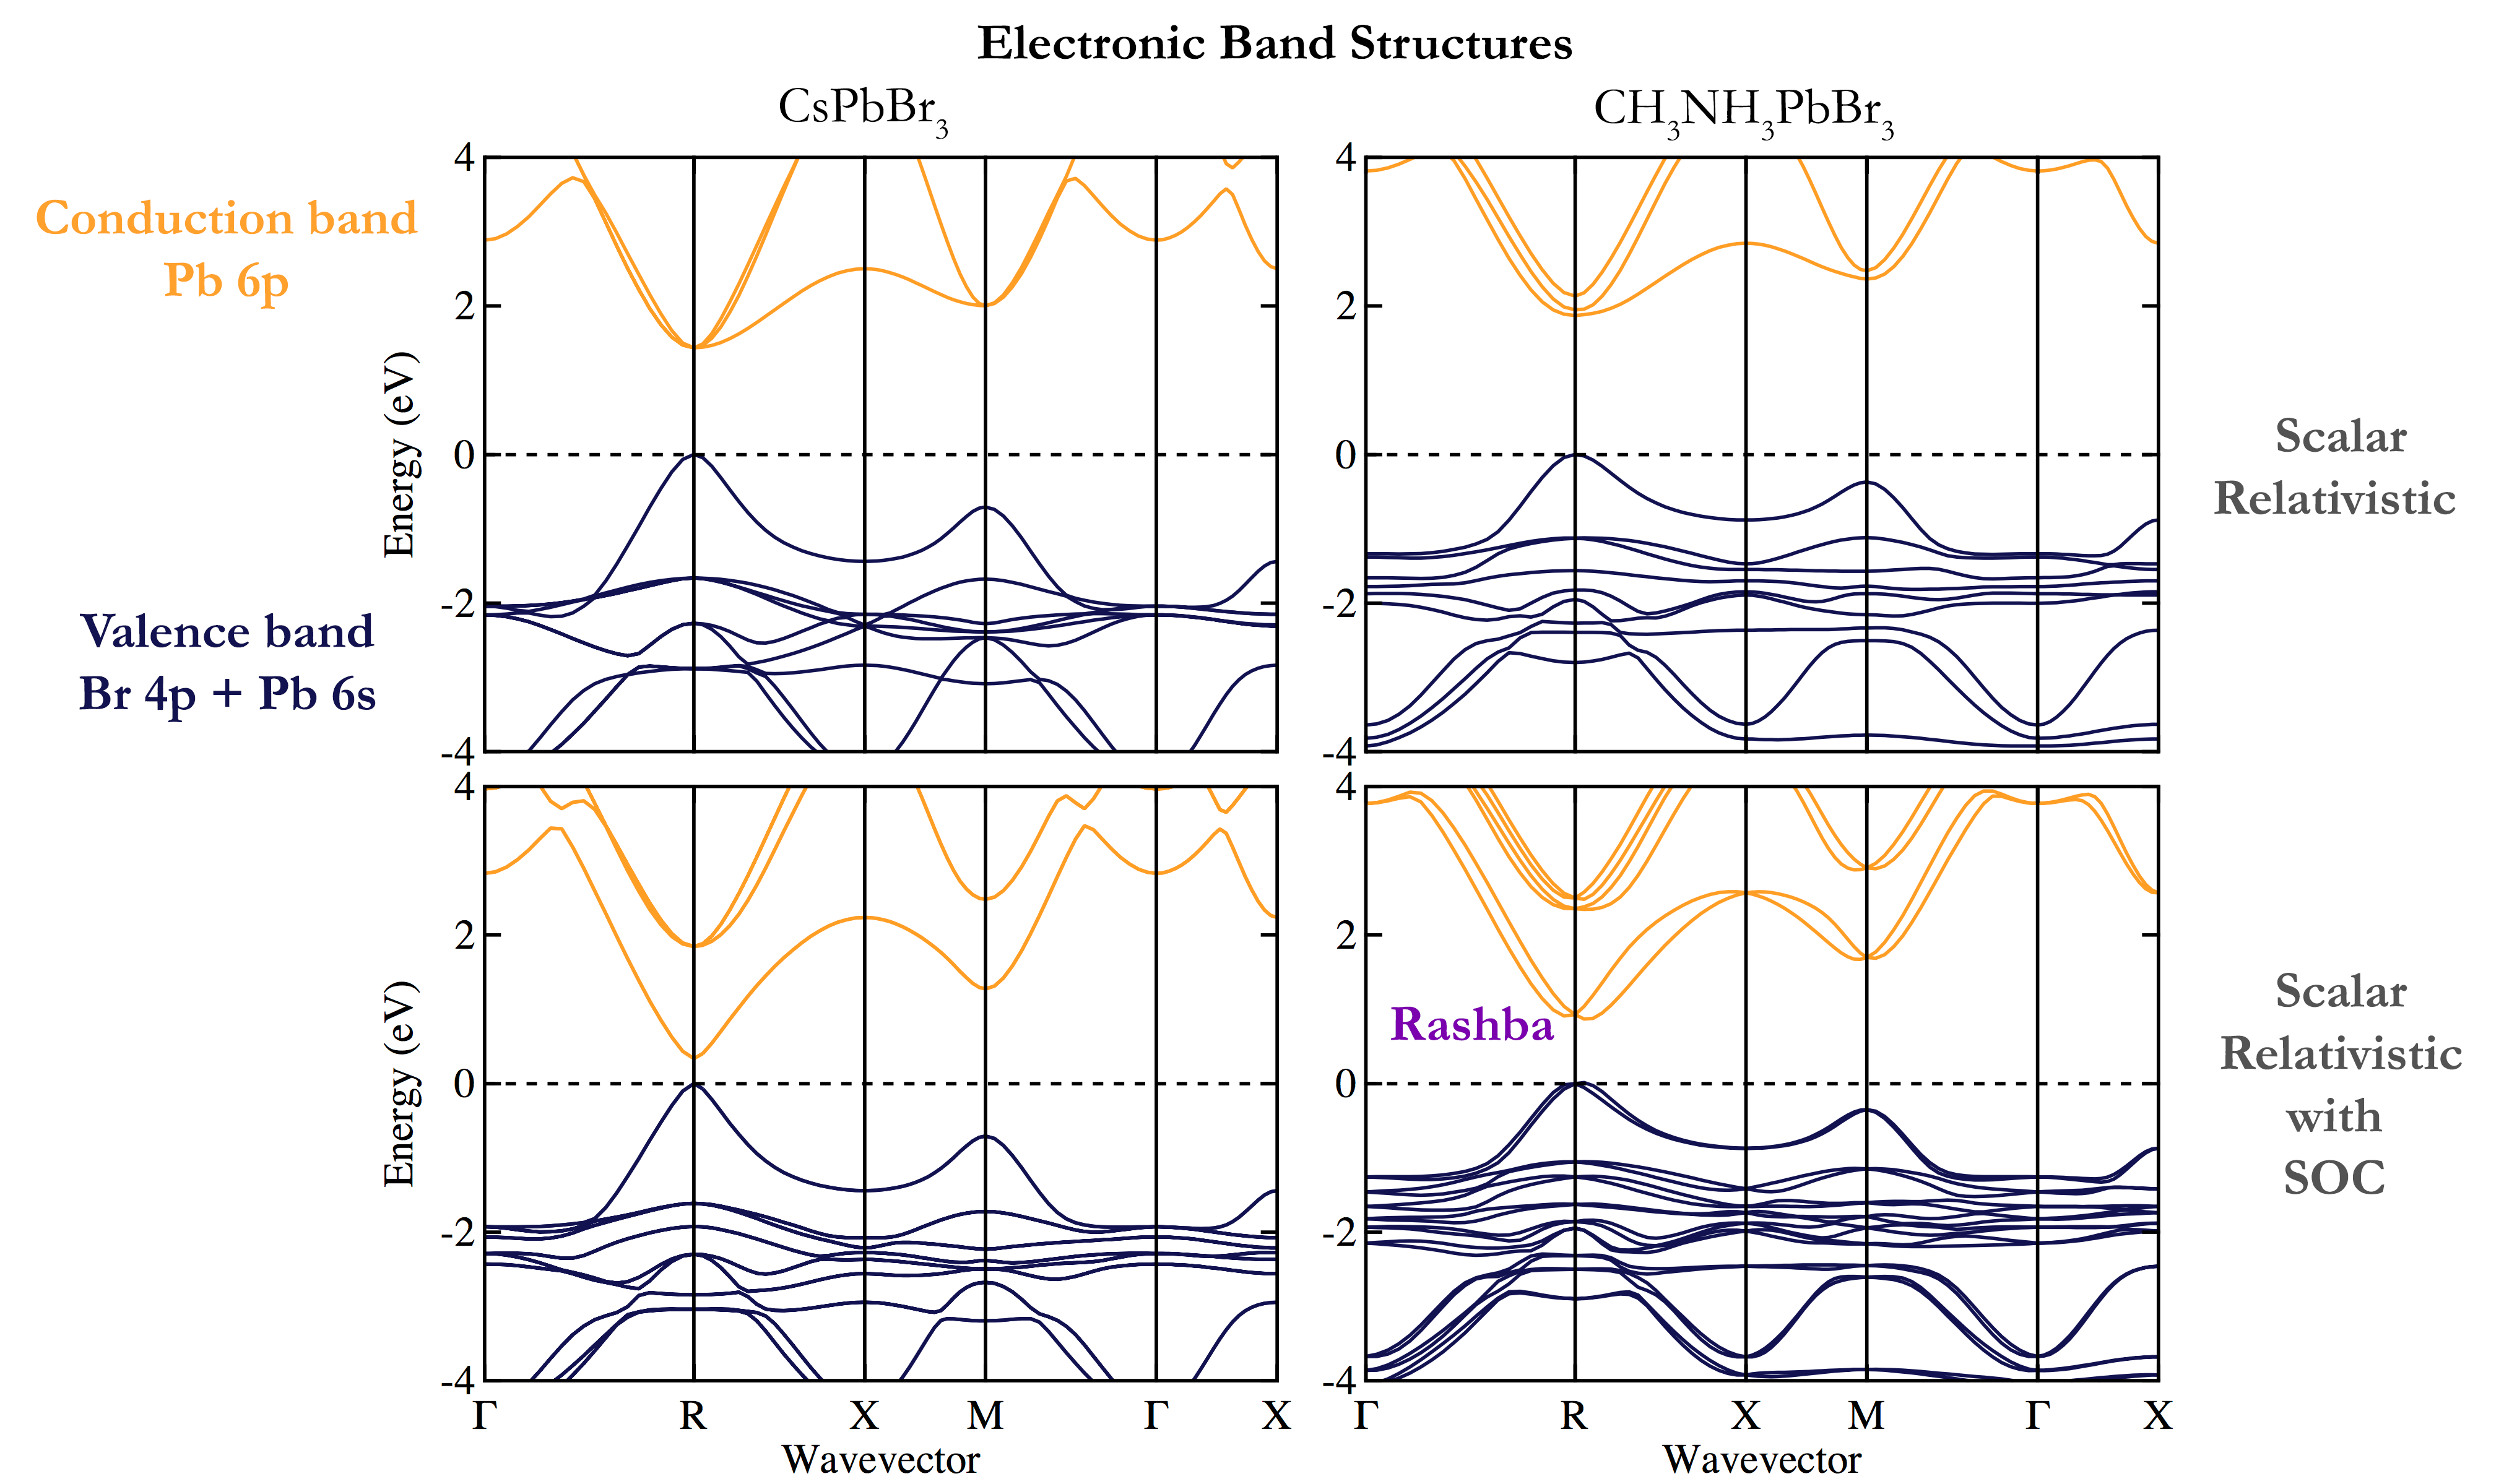
\includegraphics[width=1.0\columnwidth]{./figures/ch2/f3.png}
\caption[Electronic band structures of \ce{CsPbBr3} and \ce{CH3NH3PbBr3}]{
The electronic band structures of the inorganic perovskite \ce{CsPbBr3} and hybrid perovskite \ce{CH3NH3PbBr3} in the cubic phase.
    One effect of the organic cation is to widen the band-gap located at the $R$ point due to the larger lattice constant. 
    Spin-orbit coupling reduces the band-gap in both materials. 
The presence of \ce{CH3NH3+} in the hybrid perovskite results in a non-centrosymmetric crystal, with an associated relativistic Rashba-Dresselhaus splitting of the lower conduction band.
While labels of the special points are those of the cubic perovskite structure (space group $Pm\bar{3}m$),  
    the static model of the hybrid perovskite formally has  \textit{P1} symmetry . 
Points equivalent for a cubic crystal (e.g. $M=\frac{1}{2},\frac{1}{2},0$; $M'=0, \frac{1}{2},\frac{1}{2}$;  $M''=\frac{1}{2},0,\frac{1}{2}$) are inequivalent here. Figure prepared by Young-Kwang Jung.
}
\label{fig3}
\end{figure*}

\subsection{Anharmonic lattice vibrations and thermal conductivity} \label{ch2anharmonic}

Kohn-Sham density functional theory is most often carried out in the Born-Oppenheimer approximation where the nuclei are static classical point charges. 
To consider thermal vibrations, expansion or heat flow the theoretical framework of lattice dynamics can be used.\autocite{Stoffel2010} 
 
In the harmonic approximation, the lattice dynamics are fully specified by second-order force-constants of individual atoms, which are then used to build the dynamical matrix. 
The eigenstates of this matrix are the normal modes of vibration with an associated phonon energy. 
Thermal expansion coefficients, system anharmonicity (e.g. \grun parameters) and the temperature-dependence of other properties can be calculated in the quasi-harmonic approximation (QHA). 
Here the lattice dynamics are harmonic at a given temperature; however, the cell volume is scaled by thermal expansion to give the first-order contribution of finite temperature effects. 

The thermal expansion coefficient of MAPI in the cubic phase has been calculated with the QHA.
The value is sensitive to the density functional used.
For example, a value of $3.0 \times 10^{-5} /K$ is calculated with the PBE functional with Tkatchenko-Scheffler dispersion corrections,\autocite{Saidi2016} while the PBEsol functional produces a value of $12.5 \times 10^{-5} /K$.\autocite{Brivio2015a} 
These compare to finite temperature scattering measures of $1.91 \times 10^{-5} /K$ by X-ray,\autocite{Baikie2013} and $13.2 \times 10^{-5} /K$ by neutron diffraction.\autocite{Weller2015} 
Even taking the smallest value above, the expansion coefficient is one order of magnitude greater than silicon,\autocite{Madelung2003} highlighting the strong deviation from harmonic behaviour in halide perovskites.

In the harmonic approximation (and similarly the QHA), the dynamic matrix eigenmodes are orthogonal and the resulting phonons are non-interacting.
Consequently phonon lifetimes are infinite as the phonons do not scatter; thermal conductivity is infinite. 
To calculate phonon-phonon scattering, and so its contribution to finite thermal conductivity, anharmonic lattice dynamics need to be considered.
A computational route is to use perturbative many-body expansion, e.g. as implemented in \textsc{PHONO3PY},\autocite{Togo2015} which includes third-order force constants. 
For MAPI, 41,544 force evaluations are required for these third-order force constants, compared to 72 for second-order (harmonic) force constants.\autocite{Whalley2016}
Consequently, these calculations are vastly more expensive. 
Using this approach phonon-phonon scattering rates are calculated to be three times larger in MAPI compared to standard covalent semiconductors \ce{CdTe} and \ce{GaAs}.\autocite{Whalley2016} 
Consequently, mean free paths are on the nanometer rather than more typical micrometer scale. 
Lattice thermal conductivity is extremely low, 0.05 Wm$^{-1}$K$^{-1}$ at 300 K.\autocite{Whalley2016}
This combination of high electrical and low thermal conductivity makes these compounds potential thermoelectric materials.\autocite{He2014,Mettan2015}

In highly anharmonic systems third-order force constants and perturbation theory may not be sufficient
to describe the true dynamics, but going further with lattice dynamics becomes prohibitive.
Besides, it is not obvious whether the fundamental tenant of lattice dynamics, of expanding in small displacements around a minimum structure, is correct for these soft and highly anharmonic materials. 
In contrast, MD treats anharmonic contributions to all orders. As MD stochastically explores the phase space, long integration times are required to sample rare events, and finite size effects mean that only phonon modes commensurate with the supercell are sampled.  
%% Low thermal conductivity is linked to material breakdown explains why all of their perovskite LEDs break very quickly (heat builds up and kills the material) - much higher currents than solar cells
% Thermal stability: aron says good article on latest advances: https://pubs.acs.org/doi/10.1021/acs.jpclett.8b00463
\section{Electronic structure}

Despite the dynamic disorder just discussed, in many respects halide perovskites display characteristics of traditional inorganic semiconductors, with a well-defined electronic band structure and electron/hole dispersion relations.
However, when the electronic structure is correctly modelled, various subtleties emerge. 

\subsection{Many-body and relativistic effects} \label{Mbre}

Perhaps surprisingly, local and semi-local exchange-correlation functionals 
provide a reasonable estimate for the band-gaps of these heavy metal halide materials.
This is due to a cancellation of errors. 
For Pb-based perovskites, the conduction band has mainly Pb 6p character. 
Due to the large nuclear charge, the electronic kinetic energy requires a relativistic
treatment, and spin-orbit coupling (SoC) becomes significant. 
The first-order effect is a reduction in band-gap by as much as 1 eV\autocite{Brivio2014a}, as the degenerate 6p orbitals are split and moved apart. 
This is shown in Figure \ref{fig3} for the bromide compounds.
The typical band-gap underestimation of GGA functionals is offset by the absence of relativistic renormalisation.

SoC is not expected to have a large impact on the structural properties of the Pb-based compounds as the (empty) conduction band is mainly affected, and the force on atoms depends on the electron density (occupied orbitals). 
Accurate force-constants can be calculated without SoC considerations.\autocite{PerezOsorio2015a}
%LW - This just claims it gives same qualtatitve picture, don't think valid to cite on this point.
%AW - Fig 6 shows the potential energy surface as a function of functional

There have been a number of electronic structure calculations considering many-body interactions beyond DFT. 
Quasi-particle self-consistent \textit{GW} theory shows that the band dispersion (and so density of states, optical character and effective mass) is considerably affected by both the \textit{GW} electron correlation and SoC.\autocite{Brivio2014a}
Some materials see only a rigid shift of band structure (retaining DFT dispersion relations)\autocite{VanSchilfgaarde2006,Butler2016} but this is not the case for hybrid perovskites.
The effect of SoC on the band dispersion of MAPI is discussed in Chapter \ref{ch:4-effmass}.

A consequence of SoC when combined with a local electric field is the Rashba-Dresselhaus effect, a splitting of bands in momentum space.\autocite{Kepenekian2015}.
This can be understood as an electromagnetic effect, where the magnetic moment (spin) of the electron interacts with a local electric field, to give rise to a force which displaces it in momentum space. 
Up and down spins are displaced in opposite directions, and this displacement is a function (in both size and direction) of the local electric field, which will depend on the local dynamic order. 
For a static structure, this is demonstrated in Figure \ref{fig3} for \ce{CH3NH3PbBr3}. 
Neglecting SoC, the cubic phase has band extrema at the $R$ point (a direct band-gap).
With SoC the valence and conduction band each split into valleys symmetrical around $R$.
The splitting is much more pronounced in the \ce{Pb} $6p$ conduction band (compared to the \ce{Br} $4p$ valence band), as expected from the $Z^4$ dependence of spin-orbit coupling.
This asymmetry in the band extrema results in direct-gap like absorption and indirect-gap like radiative recombination which is discussed later.
For a comparison between SoC and non-SoC bandstructures across a range of materials see Appendix \ref{app:2-bandstructures}.

The relativistic spin-splitting can only occur in crystals that lack a centre of inversion symmetry, a prerequisite for generating a local electric field. 
The cubic representation of \ce{CsPbBr3} has an inversion centre, so while SoC affects the band-gap through the separation of Pb 6p into p$_{\frac{1}{2}}$ and  p$_{\frac{3}{2}}$ combinations,
no splitting of the band extrema away from the high symmetry points is observed (see Figure \ref{fig3}).
This is true only for a static cubic structure and, as discussed earlier, hybrid halides will have continuous local symmetry breaking. 

%It is possible that the Rashba characterisitics of hybrid halide perovskites could be exploited for use in an intermediate band solar cell. The recombination protected pockets could produce a region where an appreciable charge density provides flux to a higher energy conduction band \autocite{frost2016b}.

Point defect calculations will be particularly sensitive to the electronic structure method used.
Neglection of SoC and self-interaction errors can result in an incorrect position of the valence or conduction band edges, thus introducing spurious errors in defect energy levels and predicted defect concentrations.
Du\autocite{Du2015} showed how for the case of an iodine vacancy, a deep (0/+) donor level is predicted for GGA without SoC,
while a resonant donor level is predicted for GGA-SoC and HSE-SoC treatments of electron-exchange and correlation.

\subsection{Electron-phonon coupling} \label{ch2epcoupling}

Going beyond the Born-Oppenheimer approximation, the interaction of the electronic structure with vibrations of the lattice can be considered. 
Electron-phonon coupling can perturb the electronic band energies (changing the band-gap), and couple electronic excitations (the hole and electron quasi-particles) into vibrational excitations (phonon quasi-particles). 
In a semiconductor, charge carrier scattering is often dominated by this electron-phonon interaction, and so the strength of these processes set a limiting value on the mobility. 
Electron-phonon coupling is often calculated in a second-order density functional perturbation theory calculated for a static (rigid ion) structure.
In the normal limit, this term is expected to dominate over the first order contribution from the acoustic deformation potential as vibrations are typically small. 

Saidi et al. sampled all non-soft harmonic phonons at the $\Gamma$ point using a Monte Carlo technique,\autocite{Saidi2016} finding significant differences with the standard perturbation theory results.
%
Electron-phonon interactions can be calculated with MD, but as with phonon-phonon scattering, 
achieving convergence with respect to electronic (\textit{k}-point sampling and basis set) 
and vibrational ($q$-point sampling and supercell size), while maintaining sufficient integration time to capture rare processes, is costly.

Recently a `one shot' method has been developed to calculate band-gap renormalization and phonon-assisted optical absorption, and applied to \ce{Si} and \ce{GaAs}.\autocite{Zacharias2016} 
Nuclei positions are carefully chosen as a representative sample from the thermodynamic ensemble, and the electronic structure is needed for this static structure only---a significant increase in computational efficiency. 
Such techniques may provide a promising method to calculate the electron-phonon coupling of complex materials, but they have not yet been tested for the family of hybrid halide perovskites or other more complicated crystal structures.

\subsection{Charge carrier transport}

Charge carrier transport in hybrid halide perovskites is now considered.
The minority-carrier diffusion length is the average length a photo-excited (or electronically-injected) carrier travels before recombining. 
In a photovoltaic device, the diffusion length must be sufficient to reach the contacts.
The minority-carrier diffusion length is a product of the diffusivity $D$ and lifetime $\tau$ of minority charge carriers, $L_d = \sqrt{D\tau}$.

Minority-carrier diffusion lengths in MAPI are reported to be considerably larger than other solution processed semiconductors.\autocite{Li2015zz}
%
Long lifetimes (large $\tau$) can be partly attributed to the `defect-tolerance' of hybrid perovsites (discussed in Section \ref{defects}), reducing the rate of ionised-impurity scattering and non-radiative recombination.  

The effective masses of electrons and holes in hybrid halide perovskites are small.
Given the effective mass of $< 0.2 m_e$,  the carrier mobility of MAPI ($< 100$ \mob) is modest in comparison to conventional semiconductors such as \ce{Si} or \ce{GaAs} ($> 1000$ \mob).\autocite{Stranks2015b}
Carrier mobility must be limited by strong scattering.

Low temperature mobility in this material reduces as a function of temperature as T$^{-1.5}$, which provides circumstantial evidence for being limited by acoustic phonon scattering.\autocite{Karakus2015,Yi2016a}
However, if only the acoustic phonon scattering (which is elastic due to the population of acoustic modes) is considered, the calculated mobility is orders of magnitude larger than experiment. 
A key realisation is that the soft nature of these semiconductors results in optical phonon modes (see Figure \ref{fig2}) below thermal energy.\autocite{Brivio2015a,PerezOsorio2015a}
Optical phonon scattering is inelastic and dominates once the charge carriers have sufficient energy to generate the phonon modes.\autocite{Leguy2016} 
Through solving the Boltzmann transport equation parameterised by DFT calculations, scattering from longitudinal optical phonons is identified as the process limiting mobility at room temperature.\autocite{Wright2016,Filippetti2016}

Mobility will be further limited by scattering from point and extended lattice defects.\autocite{Ball2016}
Fluctuations in electrostatic potential resulting from dynamic disorder provide a macroscopic structure from which carriers will also scatter.\autocite{Frost2014,Ma2014d}

\begin{figure*} 
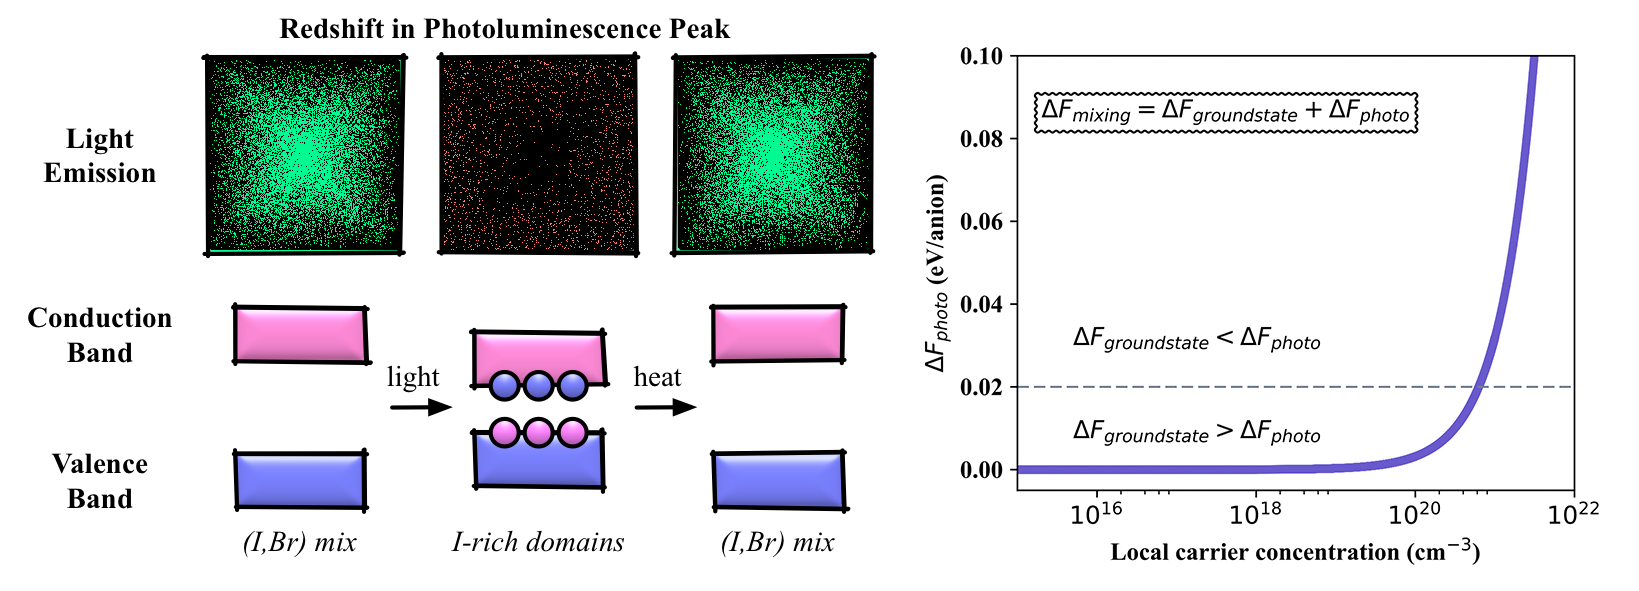
\includegraphics[width=1.0\textwidth]{./figures/ch2/f4.png}
\caption[Simple phase segregation model]{
Halide perovskites are mixed ionic-electronic conductors. The vacancy-mediated diffusion of halide anions has been associated with both current-voltage hysteresis of solar cells and the rapid interchange between iodide, bromide and chloride materials.
One point of controversy remains the reversible ion segregation observed in mixed (Br,I) systems. 
Alloyed materials have been found to phase separate upon illumination, but recover their initial state when the light source is removed. 
The phase separation is associated with a striking red-shift in  photoluminesence spectra.
A statistical mechanical analysis of ground-state DFT calculations suggested a large miscibility gap \autocite{Brivio2016}, while the charge carriers generated upon illumination can provide an additional driving force for phase separation.\autocite{Slotcavage2016}
The results from a simple thermodynamic model are shown in the right panel, where the free energy of mixing contains contributions from the ground-state with an additional component due to the difference in band-gaps between the mixed (I,Br) and phase separated I-rich phases. 
The latter contribution requires local carrier concentrations approaching 10$^{21}$ cm$^{-3}$ to make a substantial contribution to the overall mixing energy. Figure prepared by Aron Walsh.
}
\label{fig4}
\end{figure*}

\section{Photophysics and solar cells}

Hybrid halide perovskites are, in the most part, being researched in the context of solar cell technology.
There are areas of the underlying physics which are not yet developed, and which may be limiting progress in the field.
Ion migration is poorly understood and has been correlated with the hysteresis effects\autocite{Eames2015a,Richardson2016} and device degradation.
In MAPI, the iodine interstitial defect has been identified as a site for charge trapping\autocite{Whalley2017b} (as reported in Chapter \ref{ch:6-defects}), but the role of impurities is not understood. 
Additionally, interfaces have not been optimised for optimal charge carrier extraction.
These issues are outlined in the following section.

\subsection{Ion migration} 

Charged point defects in the bulk allow for mass transport of ions and can result in spatial fluctuations of electrostatic potential.
For solid-state diffusion to be appreciable in magnitude, there needs to be a high concentration of defects and a low activation energy for diffusion. 

The equilibrium concentration of charged vacancy defects is calculated as being in excess of 0.4\% at room temperature in MAPI.\autocite{Walsh2015}
Low defect formation energies and free-carrier concentrations found across the halide hybrid perovskites indicate that Schottky defects are prevalent across this family of materials.
While each point defect is charged, they are formed in neutral combinations so that a high concentration of lattice vacancies does not require a high concentrations of electrons or holes to provide charge compensation. 

The ion migration rate is given by:
%
\begin{equation}
\Gamma = \nu \textrm{exp} \left( \frac{-\Delta H^\textrm{diff}}{k_\mathrm{B}T} \right)
\end{equation}
%
where $\Delta H^\textrm{diff}$ is the activation energy for solid-state diffusion,
and $\nu$ is the attempt frequency. 
In MAPI the diffusion of methylammonium cations, iodide anions and protons have been considered in the literature. 
Activation energies calculated from first principles show that the predominant mechanism for ion migration is the vacancy assisted hopping of iodide ions.\autocite{Eames2015a}
This has been confirmed using string simulations\autocite{Meloni2016a} which, like the nudged elastic band method, calculate minimum energy paths and from this infer transition rates.

Based on a bulk activation energy of 0.58 eV\autocite{Eames2015a}, a rate of 733 hops per second would be expected at T = 300 K, with an associated diffusion coefficient of 10$^{-12}$cm$^{-2}$s$^{-1}$.
Effective activation energies as low as 0.1 eV have been reported experimentally,\autocite{Bryant2015,Game2017} which likely 
correspond to diffusion along extended defects (dislocations, grain boundaries, surfaces)\autocite{Shao2016a,Yun2016}.
The corresponding diffusion rate of 10$^{-5}$cm$^{-2}$s$^{-1}$ is very fast, but comparable to surface 
diffusion of iodine observed in other compounds.\autocite{Chandra1980}

Modelling ion diffusion at device scales is not yet possible with \emph{ab-initio} methods.
Parametrised drift-diffusion modelling of ion and electron density indicate that slow moving ions can explain the slow device hysteresis.\autocite{VanReenen2015,Richardson2016} 
A vacancy diffusion coefficient of the order of 10$^{-12}$cm$^2$s$^{-1}$ is consistent with both predictions and transient measurements.\autocite{Eames2015a}

It has been suggested that ion migration within mixed-halide compositions is the result of a non-equilibrium process induced by photoexcitation.
X-ray diffraction measurements by Hoke et al.\autocite{Hoke2015} show that under illumination the mixed halide perovskite $\ce{MAPb(I_{1-x}Br_x)3}$ segregates into two crystalline phases, one iodide-rich and the other bromide-rich.
This segregation leads to reduced photovoltaic performance via charge carrier trapping at the iodide-rich regions.
In some reports, after a few minutes in the dark the initial single phase XRD patterns are recovered. 
This reversible process is unusual and defies the common assumption made that ion and electron transport are decoupled.

A schematic outlining the phase segregation process is shown in Figure \ref{fig4}.
A phase diagram constructed from first-principles thermodynamics found a miscibility gap for a range of stoichometries at room temperature.\autocite{Brivio2016}
This suggests that a mixed-halide material is metastable and will phase segregate after being excited by light, which follow a decreasing free energy gradient towards halide-rich areas formed prior to light excitation (such as grain boundaries).
The accumulation of charge carriers increases lattice strain and drives further halide segregation.  
Our calculations indicate that the transition between mixing and segregation will occur at a local carrier concentration of $10^{21}$ cm$^{-3}$, so that charge accumulation in small regions of the material is required for this model. 

\subsection{Electron-hole recombination} \label{EHR}

The open-circuit voltage (V$_\textrm{oc}$) of a solar cell is determined by the rate of charge carrier recombination in the material, as no photogenerated charges are being extracted and so all are recombining. 
When operating to generate power, the rate of recombination competes with the rate of charge extraction, limiting the fill factor of the solar cell. 

Recombination is usually separated into three channels: 
non-radiative; radiative; and Auger (see Section \ref{exprecombo} for further dicussion). While non-radiative recombination is limiting in many inorganic thin-film technologies, hybrid perovskites are not significantly affected. 
This is surprising given the high density of defects expected
for a material processed from solution, leading to hybrid perovskites being described as `defect tolerant'. \autocite{Berry2016}

%% AW - I think explaining the concepts below properly will be too long and off topic here
%
%The external quantum efficiency as measured by electroluminescence ($EQE_{EL}$) provides a comparative measure of the rate of non-radiative recombination. 
%This is measured in the dark under an applied bias so that the device is operating as a light-emitting diode.\autocite{Tress2014a}
%\textbf{An $EQE_{EL}$  of 0.5\% \autocite{Bie2016a} is measured for MAPI. 
%[JMF: Not sure if this is true; there are similar efficiency OPVs. Still only 1 in 200 electron/hole pairs emits. GaAs is many percent.]
%Under AM 1.5 G sunlight this gives a $V_{OC}$ of $1.18V$ compared to a theoretical maximum of $1.32V$ in the Shockley-Queisser limit.  [JMF: Shockley-Queisser? relative to what?]. 
%LW - TODO: figures for Voc and EQE_EL for CdTe and CZTS.

Radiative (bimolecular) recombination is slower than would be expected for a direct band-gap semiconductor. 
%
Recent calculations reveal how relativistic Rashba splitting can suppress radiative recombination at an illumination intensity relevant to an operating solar cell.\autocite{Azarhoosh2016, Zheng2015} 
After photoexcitation, electrons thermalise to Rashba pockets in the conduction band minima away from the high symmetry point in reciprocal space.
This leads to an indirect charge recombination pathway as the overlap in $k$-space between occupied states near upper valence and lower conduction bands diminishes.
It has also been suggested that direct recombination is suppressed at very short timescales due to the pockets of minima being spin-protected.\autocite{Zheng2015}
% JMF: *cough* might be true for the first 50 fs; thereafter not true, once spins re-thermalised.
Direct gap radiative recombination is reduced by a factor of 350 at solar fluences, as electrons must thermally repopulate back to the direct gap.\autocite{Azarhoosh2016}
This is in agreement with the temperature-dependence of the bimolecular rate measured experimentally \autocite{Hutter2016a} and calls into question the validity of models where a global radiative recombination rate independent of carrier concentration is used.
Auger recombination is only significant at fluences well above solar radiation. 

Ferroelectric effects could contribute to electron-hole separation due to electrostatic potential fluctuations in real space.
Although the molecular cation plays no direct role in charge generation or separation it could influence charge transport through the formation of polar domains.\autocite{Frost2014b,Ma2014d}
This dynamic polarisation has been explored using a model Hamiltonian parameterized for the inter-molecular dipole interaction in MAPI.\autocite{Frost2014}
This model predicts the formation of antiferroelectric domains that minimise energy via dipole-dipole interaction, and dominate a cage-strain term preferring ferroelectric alignment.\autocite{Leguy2015b}
The domains would provided electrostatically preferred pathways for electrons and holes to conduct.

%By following detailed balance arguments\autocite{Shockley1961a} radiative recombination is unavoidable and provides a fundamental limit to device efficiency as a function of bandgap.
%The Shockley-Queisser limit for photovoltaic conversion efficiency is reached when all radiation is through radiative channels. 
%Non-radiative recombination, where light energy is transformed into heat, could in theory be zero.
%this is ignoring techniques designed to beat this limit \autocite{Green2017} such as multi-junction cells and multiple charge generation.
%However, there are many pathways by which non-radiative recombination may happen and this has limited the performance of other thin-film technologies  based upon materials such as \ce{CdTe} and \ce{Cu2ZnSnS4}.

\subsection{Defect levels in the band-gap}\label{defects}

To understand why defects appear to have a minimal impact upon charge carrier mobility and lifetime,\autocite{Brandt2015a} the defect properties of hybrid perovskites can be considered.
Under the Shockley-Read-Hall model for semiconductor statistics non-radiative recombination is mediated through deep defect states in the gap.\autocite{PhysRev.87.835}
Shallow defect states can act as traps but the carriers are thermally released to the band before recombination can occur.
Hybrid perovskites -- with high dielectric constant and low effective mass -- show a tendency towards benign shallow defects under the hydrogenic model:\autocite{Yu1996}
%
\begin{equation} \label{hydeqn}
E_n = - \frac{m^*}{m_0}\frac{1}{2n^2\epsilon_0^2}
\end{equation}
%
where $\frac{m^*}{m_0}$ is the effective mass ratio, $\epsilon_0$ is the static dielectric constant and $n$ is an integer number that labels the energy level. Atomic units are used and so the energy $E_n$ is given in Hartrees. 
%This corresponds to the formula for energy levels in hydrogen, with an effective mass introduced to account for dispersion due to the band and a dielectric constant to account for charge screening\autocite{Kohn1955}.
%A similar result can be obtained for acceptor states.

In Table \ref{tab:defectlevels} the first hydrogenic defect levels for MAPI, Si and CdTe are given.
The binding energy for MAPI is only 3 meV.
For ionic materials, one would expect a large central cell correction that could result in much deeper levels, as seen for the colour centres in alkali halides.\autocite{Stoneham1975}
However on-site electrostatic potentials in the I-II-VII$_3$ perovskites are relatively weak due to the small charge of the ions (e.g \ce{Cs+Pb^2+I^-_3}) compared to other perovskite types (e.g. \ce{Sr^2+Ti^4+O^2^-3}),\autocite{Brivio2014} which supports the existance of shallow levels. 
In addition, arguments based on covalency have also been proposed.\autocite{Brandt2015a}

\begin{table} \centering
\caption[Donor defect levels in \ce{CH3NH3PbI3}, Si and CdTe]{\label{tab:defectlevels}The first shallow donor defect level in \ce{MAPI}, \ce{Si} and \ce{CdTe} calculated from effective mass theory using Equation \ref{hydeqn}. The dielectric constant $\epsilon_0$ is an important descriptor for photovoltaic materials as several important properties (e.g. rate of impurity scattering) scale with its square.}
\begin{tabular}{@{}llll@{}} \toprule   %@{} removes space to the vertical edges
Material & $\frac{m^*}{m_0}$ & $\epsilon_0$ & $E_1 (meV)$ \\
\midrule
MAPI & 0.15\autocite{Frost2014b} & 25.7\autocite{Frost2014b} & 3 \\
Si & 0.45\autocite{Hava2007} & 11.7\autocite{Hava2007} &  45 \\
CdTe & 0.11\autocite{Wang2007} & 10.2\autocite{Madelung2003} & 14 \\
\bottomrule
\end{tabular}
\end{table}


\subsection{Beyond the bulk: surfaces, grain boundaries and interfaces}
% LW - Schematic: IP's against other contact materials.
% LW - Schematic from Keith's screening technique?

As perovskite solar cells approach commercial viability,\autocite{Park2016} there are considerations to be made beyond the bulk material.
Surfaces, grain boundaries and interfaces will influence device performance and long-term stability, and become increasingly important as the science is scaled up from lab to production line. 
Halide migration, ion accumulation, charge carrier transport and charge carrier recombination at the defect states are some of the processes to consider when building an accurate interface model.
There has been preliminary work, that provides insights, but real systems offer much deeper complexity. 

Perovskite films fabricated through solution processing methods are multicrystalline and so the formation of grain boundaries is inevitable.
The resulting microstructure provides pathways for ion conduction, electron-hole separation and recombination.
Improved device performance with increasing grain size\autocite{Chen2016} is evidence for shallow traps associated with the grain boundary. % LW -  for more proof: Kim et al Adv. materials 28, 917 (2016) and Hirozaku
%
Initial calculations suggest that grain boundaries do not introduce deep defects and consequently have negligible effect upon the rate of non-radiative recombination.\autocite{Yin2015b}
This is in conflict with spatially resolved photoluminescence\autocite{deQuilettes2015a} and cathodoluminescence\autocite{Bischak2015a} measurements which evidence greater non-radiative loss at grain boundaries.
Nonadiabatic MD and time-domain density DFT\autocite{Long2016a} indicate that grain boundaries localize the electron and hole wavefunctions and provide additional phonon modes.
This leads to increased electron-phonon coupling which in turn will give a higher rate of non-radiative recombination. 
%Chlorine passivation at grain boundaries was shown to restore the recombination rate found in pristine  \ce{CH3NH3PbI3} and this has been verified experimentally \autocite{deQuilettes2015a}.
%Grancini work here: microstructure on the formation of excitons

A commonly used hole transport material is spiro-OMeTAD. This material is hygroscopic so stability in humid air is a concern,\autocite{Tai2016}
and screening procedures have been used to identify alternative contacts.\autocite{Butler2016a, Murray2015a} 
Band alignment, lattice match and chemical viability via the overlap of atomic positions are used to determine the electronic-lattice-site (ELS) figure of merit.\autocite{Butler2016a}
Using this approach \ce{Cu2O} is identified as a possible earth abundant hole extractor, whilst oxide perovskites such as \ce{SrTiO3} and \ce{NaNbO3} are identified as possible electron extractors.
As with the majority of screening techniques, the candidate materials meet the necessary but perhaps not sufficient conditions. 
Further refinements to the screening procedure could consider the change in electronic properties as lattice strain and chemical inhomogeneity at the interface is introduced.

% LW - could add:
% Interface between MAPI and water?? OR
%
% Formation of protection layer: PbI (ganose and savory work).
% Excess \ce{PbI2}, which is distributed at the interface, when solution processing using \ce{MAI} and \ce{PbI2} precursor has shown to improve performance)
% An improved coupling between the \ce{TiO2} and perovskite was found when the perovskite was terminated with \ce{PbI2}, simulating the non-stochiometric material \autocite{Mosconi2016}.




\section{Summary}

I have outlined the physical properties which make hybrid perovskites unique semiconductors that are a challenge for theory and simulation. 
Common issues that can arise in the simulation of hybrid perovskites are summarized in Table \ref{tab:techsol}.
%
The volume of work in this area means that all active areas of research cannot be addressed, including perovskite-like structures with lower dimensionality (e.g. Ruddleston-Popper phases)\autocite{Tsai2016,Saparov2016b,Ganose2015} and double perovskites with pairwise substitutions on the B site,\autocite{Savory2016,McClure2016a,Wei2016a,Volonakis2016} 
which are both attracting significant interest. 
%include here that there are on average 10 papers a day?!

The properties of hybrid halide perovskites which are difficult to model are also those which make them a successful PV material.
For example, calculating ground state electronic properties using the approximation of a single static lattice does not capture the effects of strong electronic-ionic coupling. However, it is this coupling which screens charge, produces a defect tolerant material, facilitates fast charge separation and suppresses excitonic states.
As another example the transport behaviour of halide ions via Schottky-like charged vacancy defects requires a multi-scale modelling approach.
However, it is these defects that provide the low free carrier background concentration necessary for high efficiencies in a p-i-n architecture.
Attempts are now being made to distill this understanding into descriptors for the large-scale screening of novel, earth-abundant, non-toxic semiconductors.\autocite{Brandt2015a,Ganose2016}

%Future challenges include further consideration of non-equilibrium processes such as photo-induced halide separation.
%A better understanding of the energy alignment between layers and the defects introduced at interfaces will provide a firmer foundation for understanding performance-limiting hysterisis behaviour. 
%The coupling between electronic and nuclear motion may also be a fruitful avenue, especially in the context of defects.
% Can you have a de-localised deep defect?? You can have a localised shallow defect!! (Shockley paper).

\begin{landscape}
\begin{table}[tb]\centering
\begin{tabular}{p{5cm}p{7cm}p{10cm}}
\toprule
Technique & Symptom & Solution \\
\midrule
Geometry  optimisation & Partial occupancy in structure files & Test different configurations and check total energy \\
Geometry  optimisation & Missing H in structure files & Include H based on chemical knowledge and electron counting  \\
Geometry  optimisation & Slow ionic convergence & Try changing algorithm type and settings \\
Electronic structure & Bandgap is too large & Include spin-orbit coupling and consider excitonic effects \\
Electronic structure & Bandgap is too small & Use a more sophisticated exchange-correlation functional \\
Electronic structure & Bandgap is still too small & Try breaking symmetry, especially for cubic perovskites \\
Electronic structure & Workfunction is  positive & Align to external vacuum level using a non-polar surface  \\
Supercell convergence & Unusual convergence behaviour & Use only even cell expansions (e.g. $2\times2\times2$) \\
Ab initio  thermodynamics & No stable chemical  potential range & No easy fix (many hybrid materials are metastable) \\
Berry phase polarisation & Polarisation is too large & Use appropriate reference  structure and pathway \\
Point defects & Negative formation  energies & Check for balanced chemical reaction and chemical potential limits \\
Point defects & Transition levels are deep in band-gap & Check supercell expansion and charged defect corrections \\
Alloyed systems & Many possible  configurations & Use appropriate statistical  mechanics \\
Lattice dynamics & Many imaginary phonon modes & Check supercell size and force convergence \\
Lattice dynamics & Imaginary modes at zone boundaries & Use mode-following to map out potential energy surface \\
Molecular dynamics & System melts or  decomposes & Check $k$-points and basis set convergence \\
Molecular dynamics & Unphysical dynamics & Check equilibration and supercell expansion \\
Molecular dynamics & No tilting observed & Use an even supercell expansion \\
Electron-phonon coupling & Values far from  experiment & Consider anharmonic terms  beyond linear response \newline theory   \\
Drift-diffusion model & Current-voltage behaviour incorrect & Consider role of fluctuating ions and electrostatic \newline potentials \\
\bottomrule
\end{tabular}
\caption[Common issues that arise in the simulation of hybrid perovskites]{\label{tab:techsol} Common issues that arise in the simulation of hybrid perovskites, sourced from members of the Walsh Materials Design Group.
}
\end{table}
\end{landscape}
\begin{savequote}[8cm]
Two MCs can't occupy the same space at the same time,
it's against the laws of physics.
\qauthor{--- Lauryn Hill, \textit{Zealots}}
\end{savequote}

\chapter{\label{ch:3-methods}Theory and methodology}

\minitoc

%% Books:

% For a really nice explanation of solid state QM basics - bloch waves, an electron in a crystal potential etc, see Lundstrom "fundamentals of carrier transport"

\section{Introduction} 

In this chapter I present the theory and methodology that underlies the work in this thesis. The chapter starts with an introduction to Density Functional Theory (DFT); first I introduce the theoretical concepts, then I provide some details about how DFT is implemented in practice. In the second part of the chapter I outline how we can use DFT energies combined with a series of post-processing steps to predict defect formation energies and charge transition levels. The chapter ends with an introduction to the theory of lattice dynamics and how this theory is used to calculate the vibrational properties of a material. 

\section{Density Functional Theory} \label{DFTtheory}

Density Functional Theory is the most commonly used electronic structure method in condensed matter physics and quantum chemistry. 
DFT can be used to predict the ground state properties of a material including electron density, total energy, equilibrium structure, vibrational frequencies, and properties relating to differences in total energy, such as defect formation energy or surface energy. 
As DFT is a ground state theory we are not able to calculate properties relating to excited states and, without further calculations such as those outlined in Section \ref{sec:latticedynamics}, results do not incorporate the effects of temperature. 

The theoretical basis for DFT was established in 1964 through the work of Walter Kohn and Pierre Hohenberg.\autocite{Hohenberg1964} This was further developed by Walter Kohn and Lu Jeu Sham to produce Kohn-Sham DFT.\autocite{Kohn1965} However it was not until the late 1980's approximations to the exchange-correlation functional were built so that DFT could be used in practice. 

There are a growing number of codes that implement DFT. 
Although some codes aspire to a blackbox approach, with the user protected from the underlying mechanics of DFT, for most systems of interest an understanding of the underlying approximations and parameters used are required for reliable results.

\subsection{Basic concepts} %expand to include more equations, including slater determinant? and E\phi=H\phi.

Firstly, a note on the name. A function accepts one or more numbers as input and produces a number as output. Likewise, a functional accepts one or more \textit{functions} as inputs, and produces a number as output. In DFT the functional is the electron density which is itself a function of space and time.

Throughout this chapter, unless stated otherwise, we use the Born-Oppenheimer approximation: the heavy atomic nuclei are treated as fixed points, and we solve the ground state quantum mechanical problem for the electrons only. This reduces the number of degrees of freedom of the system, a tactic that will be used again later in the chapter.

Although no one single text is followed, concepts for the underlying theory have been taken from References \cite{Burke2007}, \cite{Scuseria05} and \cite{Perdew2010}.


\subsubsection{The Schr\"{o}dinger equation}

A fundamental postulate of quantum mechanics is that for any physical system there is an associated wavefunction that contains all the system information.
The Schr\"{o}dinger equation describes the wavefunction $\Psi$ of a quantum mechanical system.  Once the Schr\"{o}dinger equation is solved, and a wavefunction is found, all the physical properties for that system follow. To take the simplest possible example, the time-independent non-relativistic Schr\"{o}dinger equation for a single particle can be written as:
\begin{equation} \label{singleparticle}
\left[\frac{-\hbar^2}{2m}\nabla^2+v_\textrm{ext}(\textbf{r})\right]\Psi(\textbf{r}) = E\Psi(\textbf{r}),
\end{equation}
where the first term in the bracket corresponds to the kinetic energy and the second term corresponds to the potential energy. For a single particle in a simple potential, such as the ``particle in a box'' system or hydrogen atom, the Schr\"{o}dinger equation can be solved exactly. Unfortunately it is not possible to solve the Schr\"{o}dinger equation exactly for more complex systems, where there are multiple electrons interacting with each other (N-body or many-body systems). In this case, the Schr\"{o}dinger equation takes the form:
\begin{equation}
\left[\frac{-\hbar^2}{2m}\sum_{i=1}^N\nabla_i^2+\sum_{i=1}^Nv_{\textrm{ext}}(\textbf{r}_i)+\sum_{i<j}^N\frac{q_iq_j}{\lvert\textbf{r}_i-\textbf{r}_j\rvert}\right]\Psi(\textbf{r}_i) = E\Psi(\textbf{r}_i),
\end{equation}
where the third term in the square bracket describes the electrostatic interaction between two particles of charges $q_i$ and $q_j$, and couples the coordinates of the particles together.

Hartree-Fock methods and Kohn-Sham DFT provide ways to obtain an approximate solution to the Schr\"{o}dinger equation for systems of interest. They do this by mapping the interacting problem onto a non-interacting problem with an effective potential $v_\textrm{ee}(\textbf{r})$. In doing so, the dimensionality of the problem is greatly reduced. Instead of solving one N-dimensional computationally intractable problem, N one-dimensional problems are solved (Figure \ref{decouple}). These methods provide a compromise between accuracy and computational efficiency.

\begin{figure}[h]
\centering
  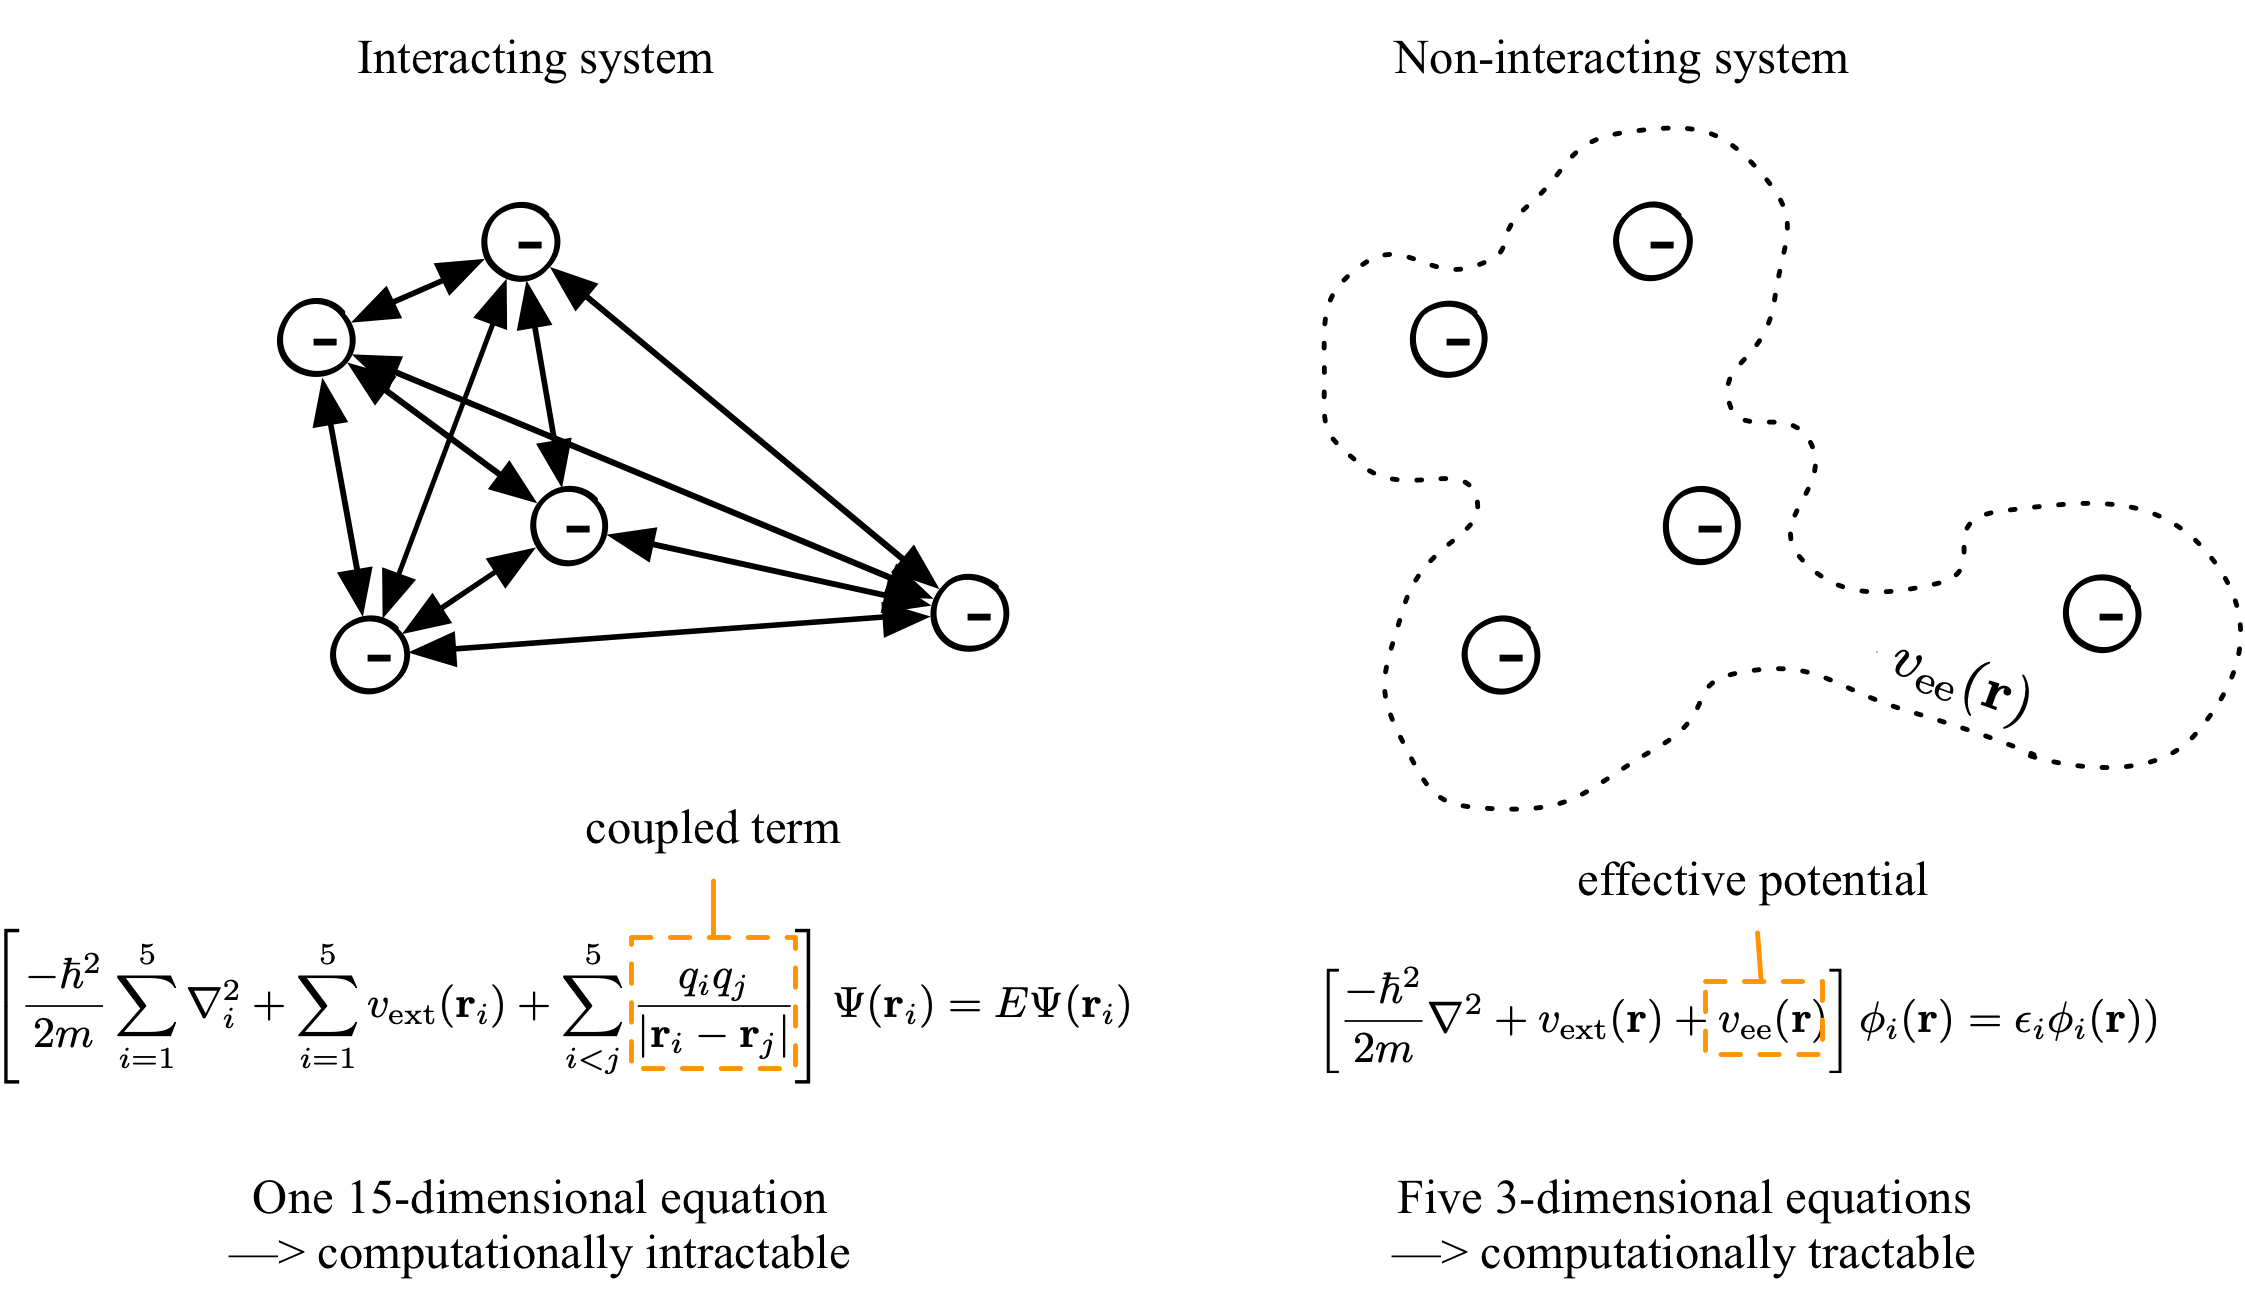
\includegraphics[width=1.0\columnwidth]{figures/ch3/decouple.png}
  \caption[Interacting and non-interacting particle systems]{Schematic outlining the equivalence between a system of interacting particles and a system of non-interacting particles in an effective potential. The underlying idea is that an interaction can be replaced by the equivalent potential. This maps the interacting 3N-dimensional problem onto N 3-dimensional problems. A consequence of this mapping is that the effective potential depends on the electron density which is itself dependent on the effective potential -- a self-consistent set of equations is formed. For the non-interacting case $\phi_i$ is used to denote a single particle wavefunction.} %update so q1q2 in couple term in picture
  \label{decouple}
\end{figure}

\subsubsection{Hartree-Fock methods}

Hartree-Fock (HF) methods introduce the concept of fictitious non-interacting one-electron orbitals $\phi$ as a way of solving the Schr\"{o}dinger equation. The one-electron orbitals are combined using a Slater determinant to produce the HF many-body wavefunction.\autocite{Burke2007} 

The effective potential, introduced in Figure \ref{decouple}, is given by $v_{\textrm{ee}} = U + E_{\mathrm{x}}$. $U$ accounts for the electrostatic interaction between electrons. Hartree-Fock methods model the charge interaction as a coulomb potential for a system of fixed electrons; the electrons feel the average electrostatic field due to the other electrons.
$E_\mathrm{x}$ accounts for the spin exchange interaction between electrons.
Electrons with the same spin are indistinguishable, and a consequence of this is that the many body wavefunction must be anti-symmetric. This leads to the Pauli Exclusion Principle, whereby two identical electrons (i.e. electrons with the same spin and momentum) cannot occupy the same space at the same time.
Hartree Fock methods account for electron exchange $E_\mathrm{x}$, the repulsion between electrons with parallel spins, exactly. 

Hartree-Fock methods do not give an exact solution to the Schr\"{o}dinger equation as the true many body wavefunction is not formed from a simple Slater determinant. As a result of using a Slater determinant, electron correlation is ignored. This is the correlated motion of electrons with anti-parallel spins as a result of their mutual coulombic repulsion.
% from http://newton.ex.ac.uk/research/qsystems/people/coomer/dft_intro.html

\subsubsection{The Hohenberg-Kohn theorems}

The 1964 Hohenberg-Kohn paper\autocite{Hohenberg1964} contains two key results: (i) the ground state electron density uniquely determines the ground state electronic wave function and, following this, all properties of the system; (ii) the true density functional for the electronic energy assumes its minimum for the correct ground-state density. % quote this from? http://publish.uwo.ca/~vstarove/PDF/tacc_chapter24.pdf

The potentials (external, coulomb and exchange) in Hartree-Fock methods determine the properties of a system. Hohenberg and Kohn demonstrate that the electron density $\rho$ can be used instead to uniquely characterise the system; rather than solving the Schr\"{o}dinger equation for the wavefunction, we can solve it for the electron density. The total energy $E\left[\rho\right]$ can be expressed as
\begin{equation}
 E\left[\rho\right]=\int v_{\textrm{ext}}(\textbf{r})\rho(\textbf{r})d\textbf{r}+T\left[\rho\right]+J\left[\rho\right]+E_{\textrm{xc}}\left[\rho\right],   
\end{equation}
where $T\left[\rho\right]$, $J\left[\rho\right]$ and $E_\textrm{xc}\left[\rho\right]$ describe the kinetic, classical electrostatic and exchange-correlation energies respectively. 
For a fixed number of electrons the functional $F\left[\rho\right]=T\left[\rho\right]+J\left[\rho\right]+E_{\textrm{xc}}\left[\rho\right]$ is universal, and the only thing that varies between systems is the external potential (determined by the electron-nuclei interaction). 

In reference \cite{Hohenberg1964} Hohenberg and Kohn also demonstrate that the ground state energy can be found variationally; the density that minimises the total energy is the true ground state density. This formalism has the advantage that the electron density has a lower dimensionality than the N-electron wavefunction (Figure \ref{dimensions}). The problem is that although the Hohenberg-Kohn theorem tells us that the terms $T\left[\rho\right]$ and $E_{\textrm{xc}}\left[\rho\right]$ exist, they are unknown and must be approximated.

\begin{figure}[h]
\centering
  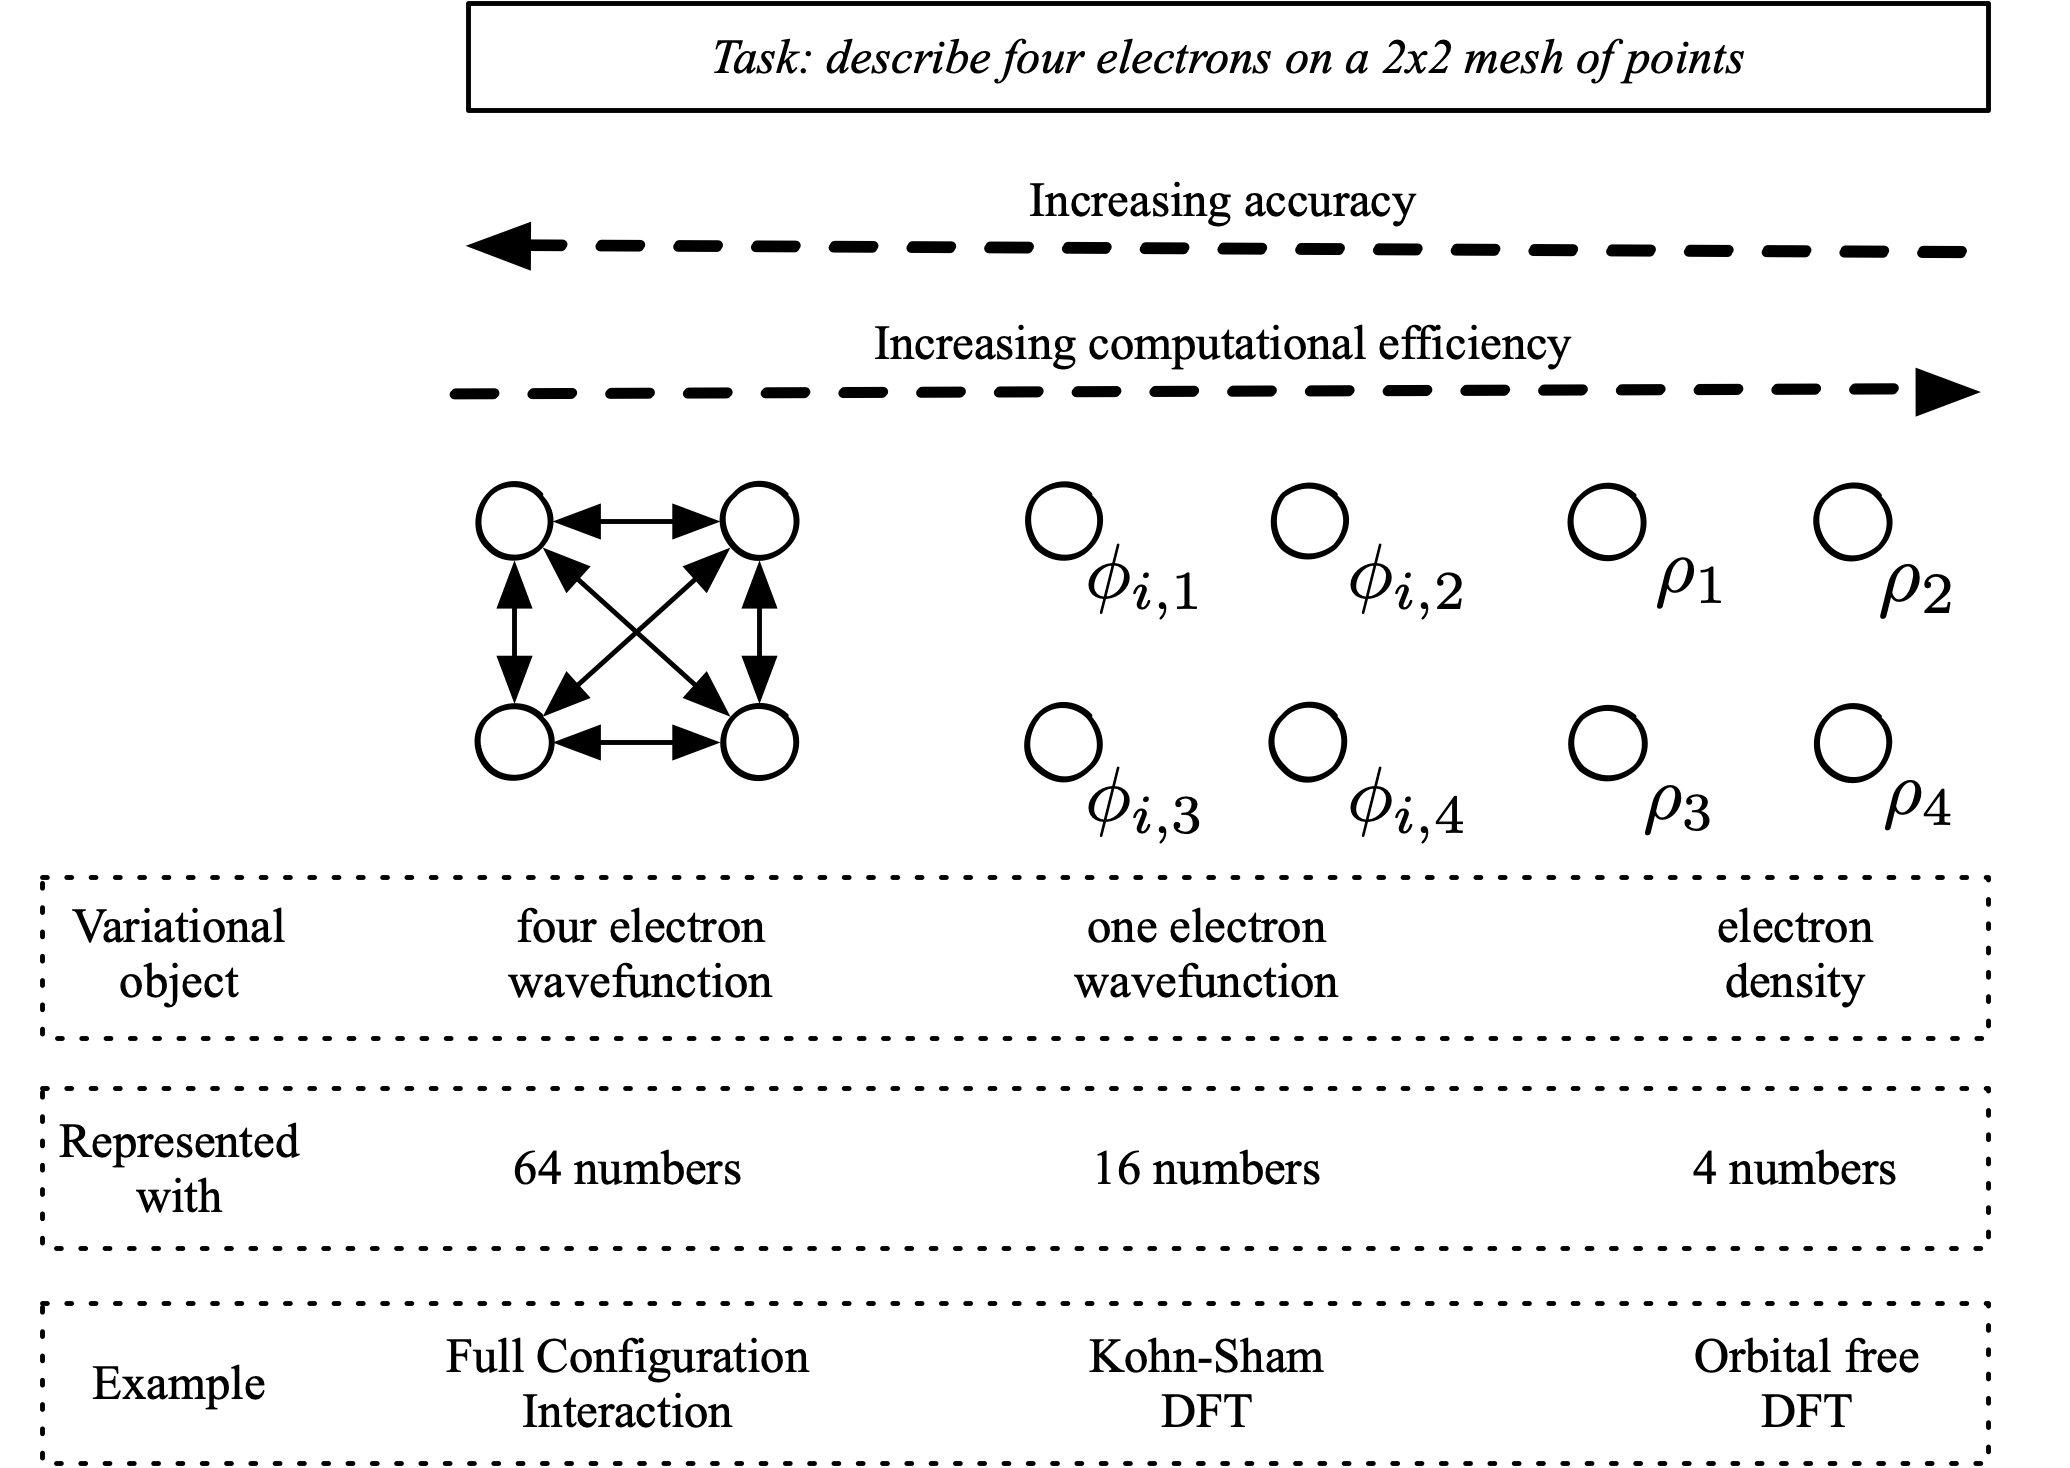
\includegraphics[width=0.8\columnwidth]{figures/ch3/dimensions.png}
  \caption[Dimensionality of variational objects]{To solve the Schr\"{o}dinger equation we can use a variational object with lower dimensionality and higher computational efficiency, although this will come at the cost of accuracy. This schematic is based on a discussion in Walter Kohn's Nobel Prize lecture.\autocite{Kohn1999}}
  \label{dimensions}
\end{figure}
% Is this right? I don't understand how the two electron wavefunction scales (4^2) - it's discussed in the 14 easy lessons.


\subsubsection{The Kohn-Sham theorem} 

The Kohn-Sham theorem shows that for any interacting system with ground state density $\rho(\textbf{\textrm{r}})$ there exists a non-interacting system with the same ground-state $\rho(\textbf{\textrm{r}})$. To find the ground state energy of the real interacting system, the occupation numbers of \textit{fictitous}, non-interacting one-electron orbitals can be optimised. For a non-interacting system we know how to calculate $T\left[\rho\right]$ and this provides a good approximation to the true kinetic energy, so the Kohn-Sham theorem provide a more practical way to apply DFT. However, the exchange-correlation density functional $E_{\textrm{xc}}\left[\rho\right]$ is still not known. Only approximations to this functional can be made, leading to approximations for the electronic density, total energy and other system properties.


\subsection{DFT in practice}

\subsubsection{Exchange-correlation functionals}
To use Kohn-Sham DFT we must approximate the exchange-correlation functional, and there is a growing list of functionals at varying levels of complexity. John Perdew proposed ``Jacob's Ladder'' as a way to categorise these functionals (Figure \ref{jladder}). As a general rule, more accurate functionals are constructed by including more parameters and variables.

\begin{figure}[h]
\centering
  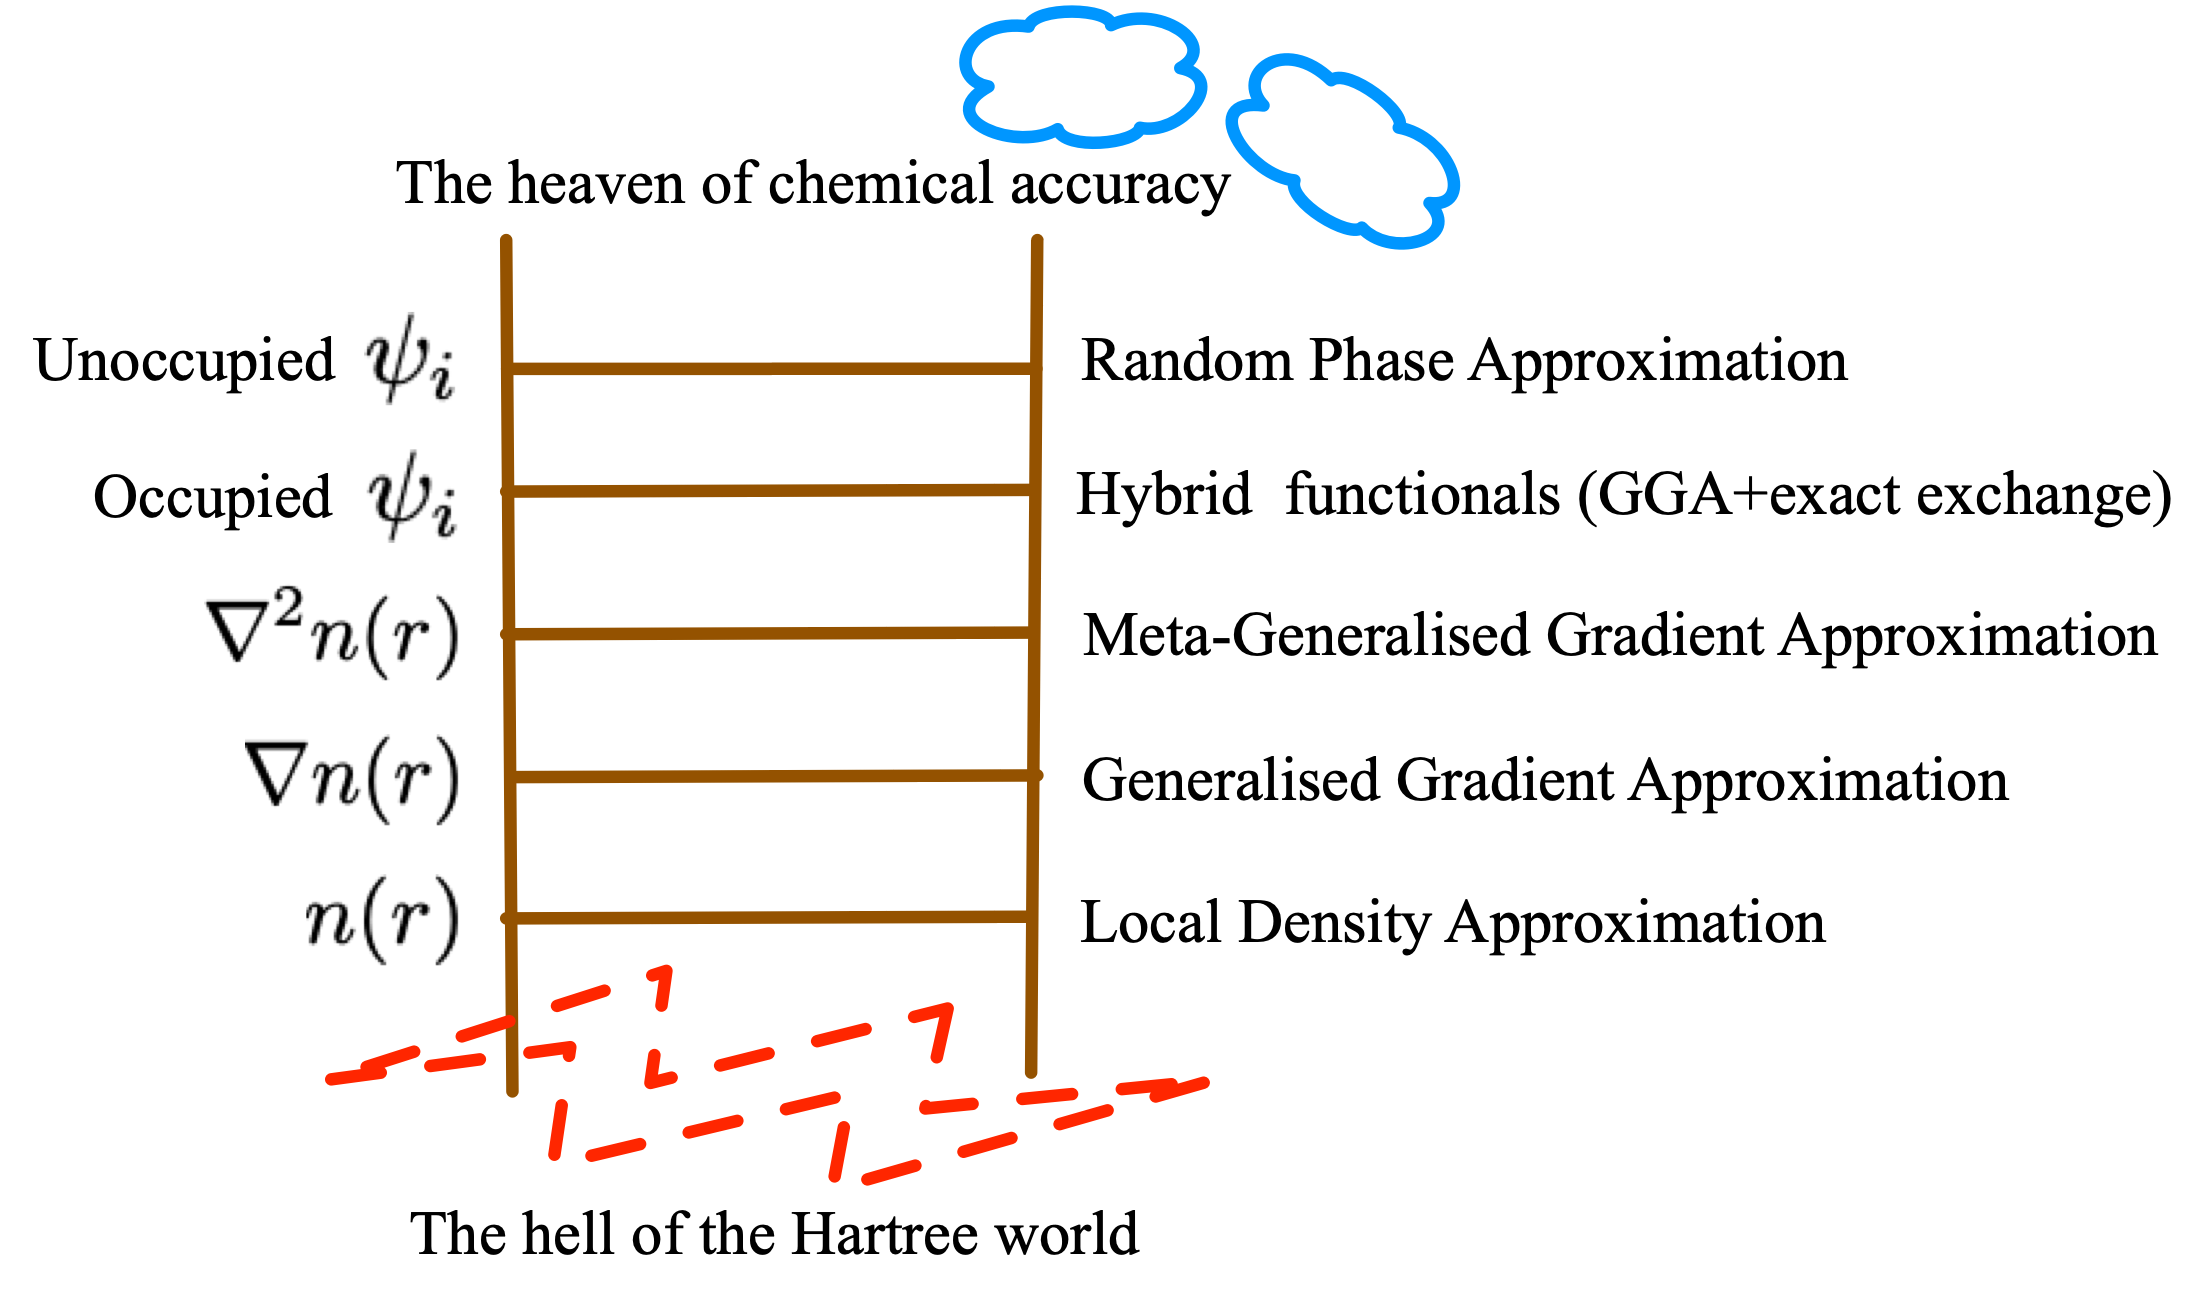
\includegraphics[width=0.8\columnwidth]{figures/ch3/jladder.png}
  \caption[Jacob's ladder of exchange-correlation functionals]{Jacob's ladder of exchange correlation functionals. On the right hand side are the various categories of exchange-correlation functionals and on the left hand side are the additional input variables included at each level of theory. As we move up the ladder the chemical accuracy increases, alongside computational expense.}
  \label{jladder}
\end{figure}


\textbf{Local Density Approximation} 

At the lowest rung of the ladder is the local density approximation where only one variable, the electron density for an infinitesimal 3-dimensional volume element, is used to calculate the exchange correlation energy. The exchange energy is calculated exactly
\begin{equation}
E_{\textrm{LDA,x}}\left[\rho\right] = {-\frac{3}{4}\left(\frac{3}{\pi}\right)^{\frac{1}{3}}\rho^{\frac{4}{3}}\left(\textbf{r}\right)d\textbf{r}},
\end{equation}
and the correlation energy is calculated numerically by fitting to many-body quantum Monte Carlo calculations for an inhomogeneous electron gas. %Ceperley and Alder
Strictly, the LDA should only be used for slowly varying densities, however it has performed surprisingly well for predicting the properties of a variety of atoms, solids and molecules. This is due to a cancellation of errors: LDA underestimates the exchange energy and overestimates the correlation energy. However there is a tendency for LDA to overestimate the binding energy and underestimate lattice parameters. This is a particularly pronounced problem in weakly bonded systems.


\textbf{Generalised Gradient Approximation}

At the next level of theory, two variables are used to determine the exchange-correlation energy: electron density and the density gradient. Due to their dependence on the GGA functionals are semi-local. The parameters of GGA functionals can be derived from physical constraints (non-empirical, as in the widely used PBE functional), or obtained from fitting procedures (empirical, as in the case of the B88 functional). GGAs improve the over-binding of LDA, but tend to underestimate the bandgap of the material.


\textbf{Meta-GGA} 

Meta-GGAs extend the GGA functional to include the non-interacting kinetic energy density as an input variable. This is the calculated from the laplacian of the occupied electron orbitals.


\textbf{Hybrid functionals} 

In DFT each electron interacts with itself as the potential derives from the total charge density of the system. This error is particularly pronounced for localised states, after trapping an electron or hole at a defect site for example. Hybrid functionals combine GGA functionals with a proportion of the exact HF exchange energy to correct the self-interaction error. The simplest hybrid functional takes the form
\begin{equation}
E_{\textrm{hybrid,xc}}\left[\rho\right] = \alpha E_{\textrm{exact,x}} + \left(1-\alpha\right)E_{\textrm{GGA,xc}}.
\end{equation}
In some studies the proportion of exact exchange is tuned to reproduce the property of interest correctly. For example, $\alpha=0.43$ is commonly used to correctly reproduce the bandgap of the hybrid halide perovskite MAPI. %
% good stuff here incl. schematic: https://www.ncbi.nlm.nih.gov/pmc/articles/PMC4892865/#S3title
% - Linked to Koopman’s linearity:E(N) – E(N-1) = En
% See Janak 1978. 

 
\textbf{Random Phase Approximation} 

Closest to heaven is the Random Phase Approximation (RPA), which uses all of the Kohn-Sham orbitals (occupied and unoccupied) as input variables. The functionals listed so far are inaccurate when there are significant long range effects, as they have no information about the electron density far from an electron. The RPA is able to correctly predict long-range interactions, such as the van der Waals interaction, between non-overlapping electron orbitals.
% can I find plot of total energy as function of seperation using different approaches??
%As DFT is exact except for the approximation to the exchange-correlation functional, any shortcoming to a DFT prediction can be attributed to the XC-functional. It should be noted though that DFT 
% DFT was not designed to calculate bandgaps.
% - However, since 2000 functionals have been better at giving total energy but they don’t give accurate density: straying away from ab-initio into a fitting exercise: DFT is straying from the path towards an exact functional

\subsubsection{Exploiting symmetry}

The material studied in this thesis, MAPI, is a crystalline solid. Although we want to understand the properties of a finite piece of material, we use the standard approach and model the finite crystal as an infinite crystal. This is acceptable if the crystal piece is large enough so that its properties do not depend on size. Born-von Karman (periodic) boundary conditions are used so that the infinite crystal is built from a repeating array of unit cells. There are an infinite number of unit cells of different shapes and sizes that can be used to build an infinite crystal. Any physically significant function of the crystal must have the same periodicity.

In real materials translational symmetry can be broken, for example when there are point defects (as in Results chapter \ref{ch:6-defects}). Furthermore, lattice vibrations have a periodicity larger than the unit cell. To model defects or lattice vibrations a supercell is built from multiple unit cells and this is used as the basic repeating unit (Figure \ref{translational}).

\begin{figure}[h]
\centering
  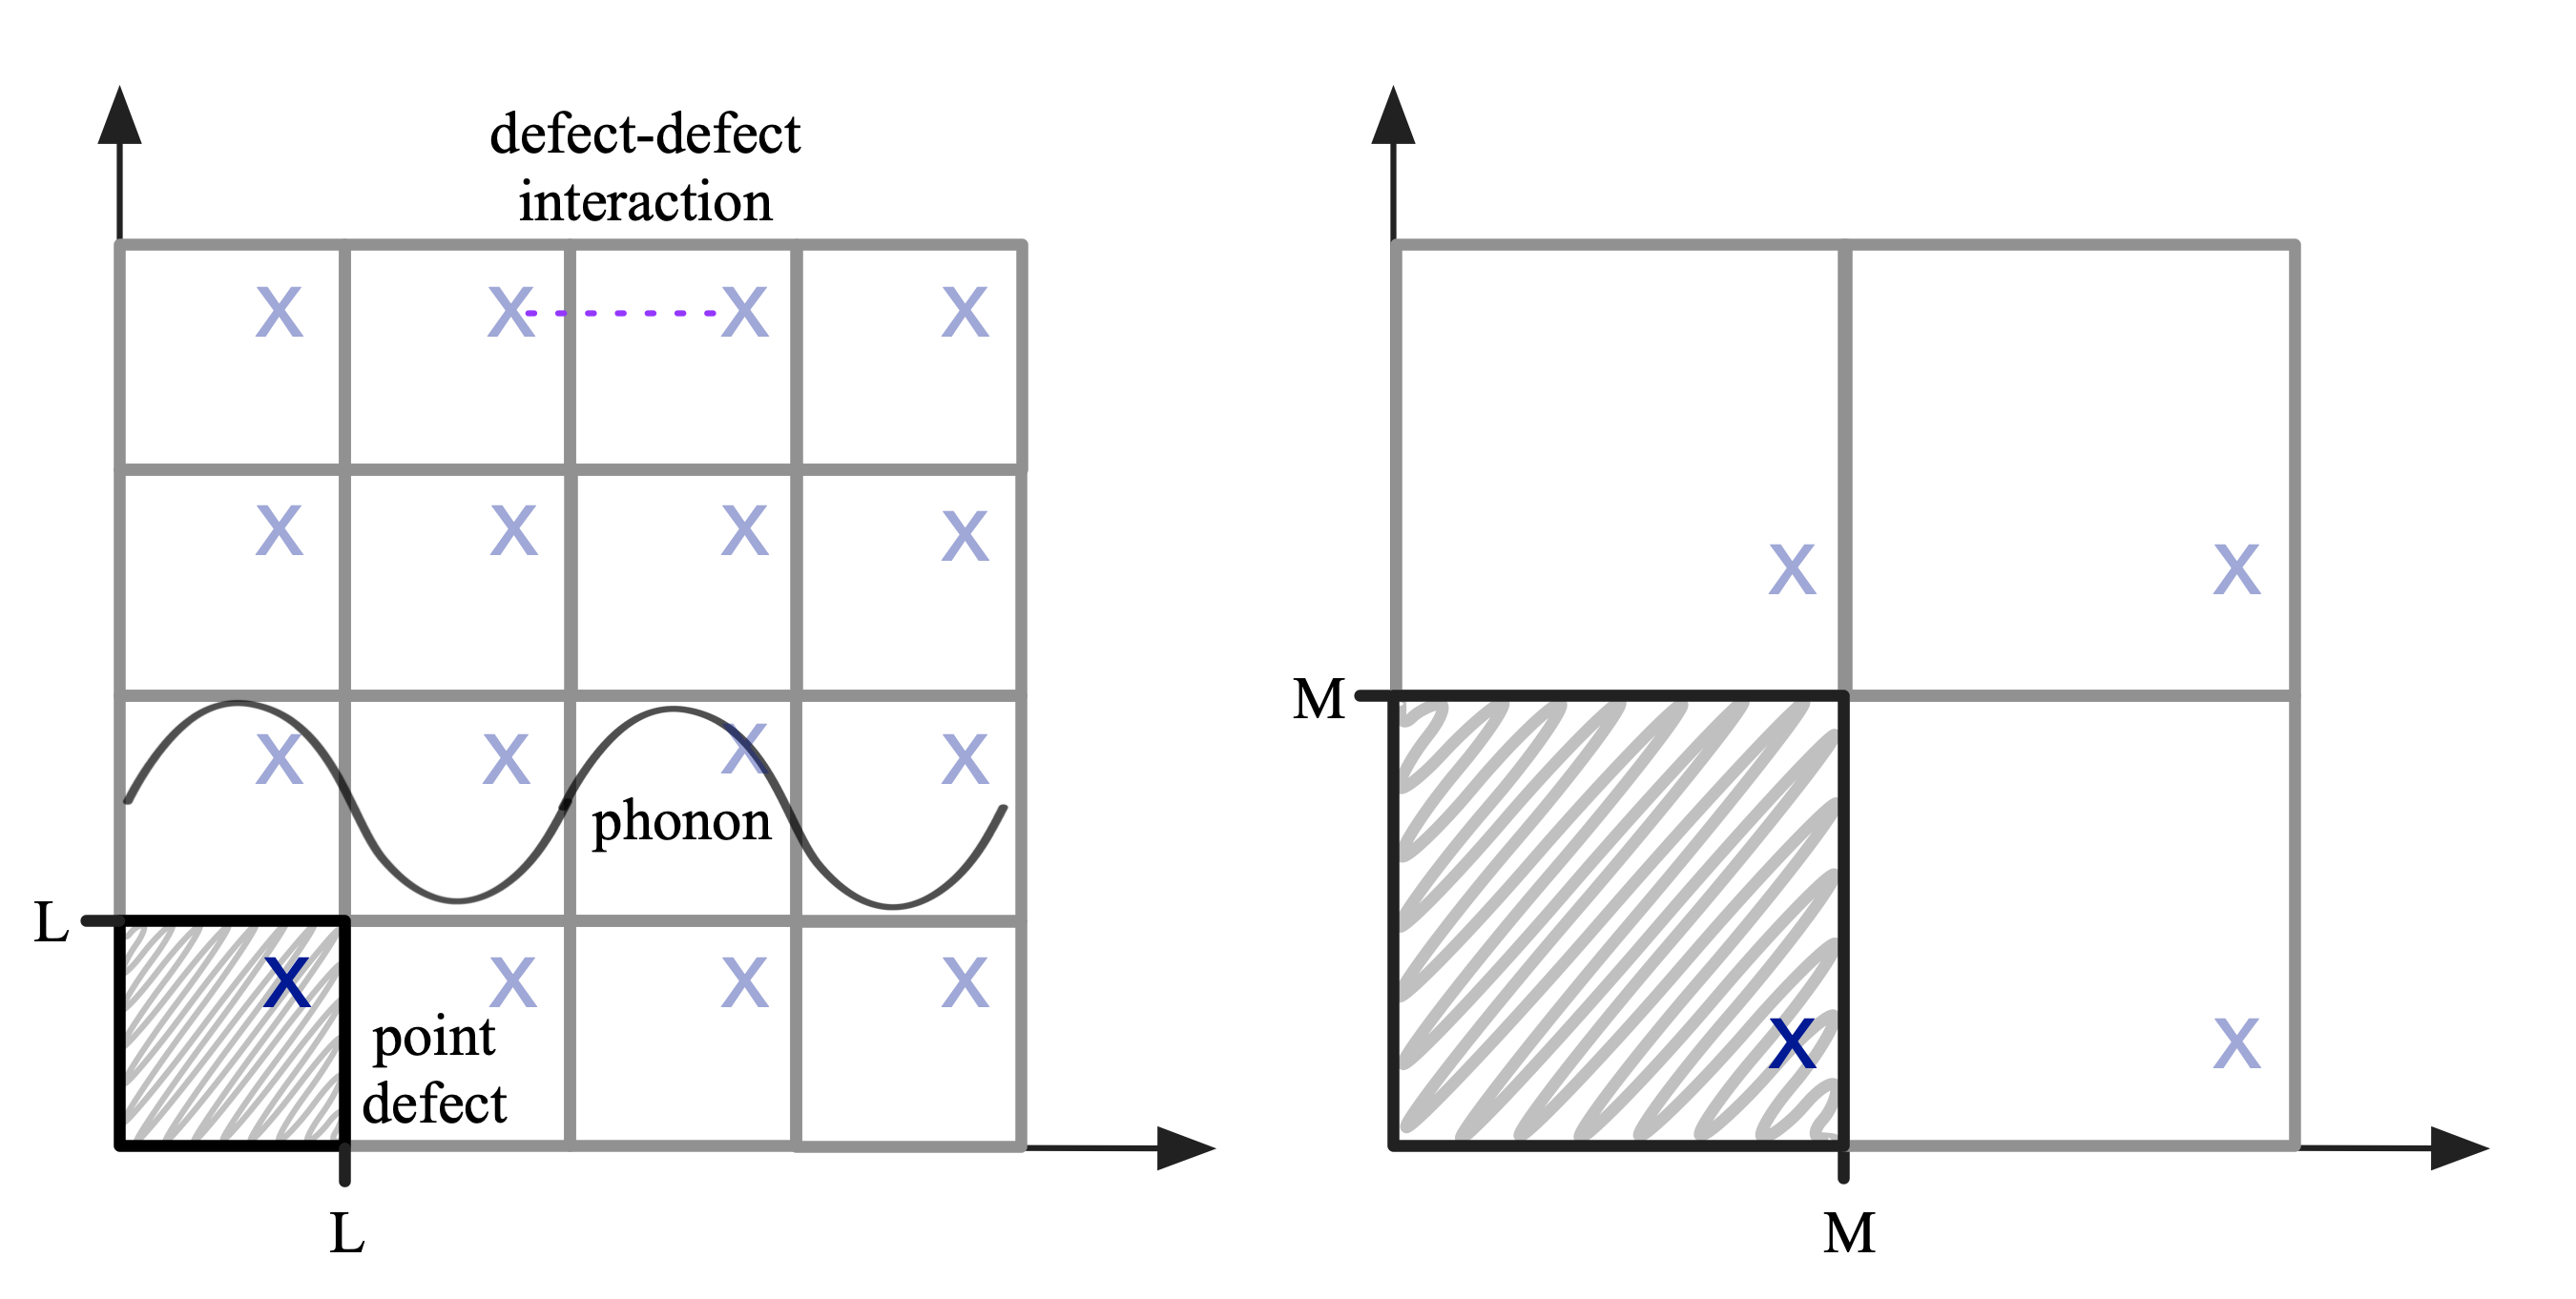
\includegraphics[width=0.8\columnwidth]{figures/ch3/supercell.png}
  \caption[Translational symmetry and supercell construction]{(LHS) An infinite crystal is built from a repeating unit cell of length $L$. Point defects (marked with an `x') break translational symmetey in real crystals and care must be taken when modelling these as neighbouring defects can interact with each other in an unphysical way. In addition, vibrational modes can have $\nu>L$ (sine wave). (RHS) A supercell of length $M=2L$ can be built to reduce defect-defect interactions and model longer wavelength phonons. } 
  \label{translational}
\end{figure}
% copy and paste phonon mode across to supercell picture?

When the Schr\"{o}dinger equation is solved for a hydrogen atom the solution gives wavefunctions corresponding to the 1$s$, 2$s$, 2$p$, etc orbitals found in chemistry. When the Schr\"{o}dinger equation is solved for a periodic system, wavefunctions are formed by Bl\"{o}ch functions $\psi_{\textbf{k}}$:\autocite{Hoffmann1987}
\begin{equation} \label{bloch}
\psi_{\textbf{k}} = u_\textbf{k}e^{i\textbf{k}\cdot\textbf{r}}.
\end{equation}   %could do a sketch of the two parts and the resulting part, and the periodic potential
The Bl\"{o}ch function is formed from the product of a basis function $u_\textbf{k}$ with the same periodicity as the crystal lattice, and a plane wave $e^{i\textbf{k}\cdot\textbf{r}}$. $\textbf k$ is the crystal wave vector which forms a space known as reciprocal space; to understand the physical significance of $\textbf{k}$ we consider an infinite 1D chain of hydrogen atoms separated at distance $L$. The electron states can be described as a linear combination of hydrogen 1s orbitals $u_n$ centred at each lattice point:

\begin{equation} \label{1dbloch}
\psi_k = \sum_nu_ne^{iknL}.
\end{equation}

$k=0$ corresponds to the lowest energy bonding state, and $k=\frac{\pi}{L}$ corresponds to the highest energy anti-bonding state
\begin{align}
\psi_0 &= \sum_nu_ne^0 = u_0 +u_1 +u_2 +u_3 \dots \\
\psi_{\frac{\pi}{L}} &= \sum_nu_ne^{i\pi n} = u_0 -u_1+u_2-u_3 \dots
\end{align}
Between these two extremes there is a continuum of states forming an electronic band (Figure \ref{bands}). 

Returning to the mathematical description of any periodic system, Equation \ref{bloch} substituted into Equation \ref{singleparticle} gives:
\begin{equation} \label{energyequation}
\left[\frac{1}{2m}\left(\frac{\hbar}{i}\nabla+\hbar \textbf{k}\right)^2+v_\textrm{ext}(\textbf{r})\right]u_\textbf{k} = E(\textbf{k})u_\textbf{k}.
\end{equation}
For any $\textbf{k}$ we can solve Equation \ref{energyequation} with periodic boundary conditions to calculate the electronic bandstructure $E(\textbf{k})$. There are an infinite number of eigenvalues $E_n(\textbf{\textbf{k}})$, where $n$ is used to label a particular eigenvalue (band). As a result of crystal symmetry, $E_n(\textbf{k})$ is periodic and only $k$-vectors within a region of space known as the Brillouin Zone ($|\textbf{k}|<\frac{\pi}{a}$) need to be considered.\autocite{Lundstrom2000} 
%talk about high symmetry points and the naming conventions (greek in zone and latin a boundaries) - choose route through use aflowlib

\begin{figure}[h]
\centering
  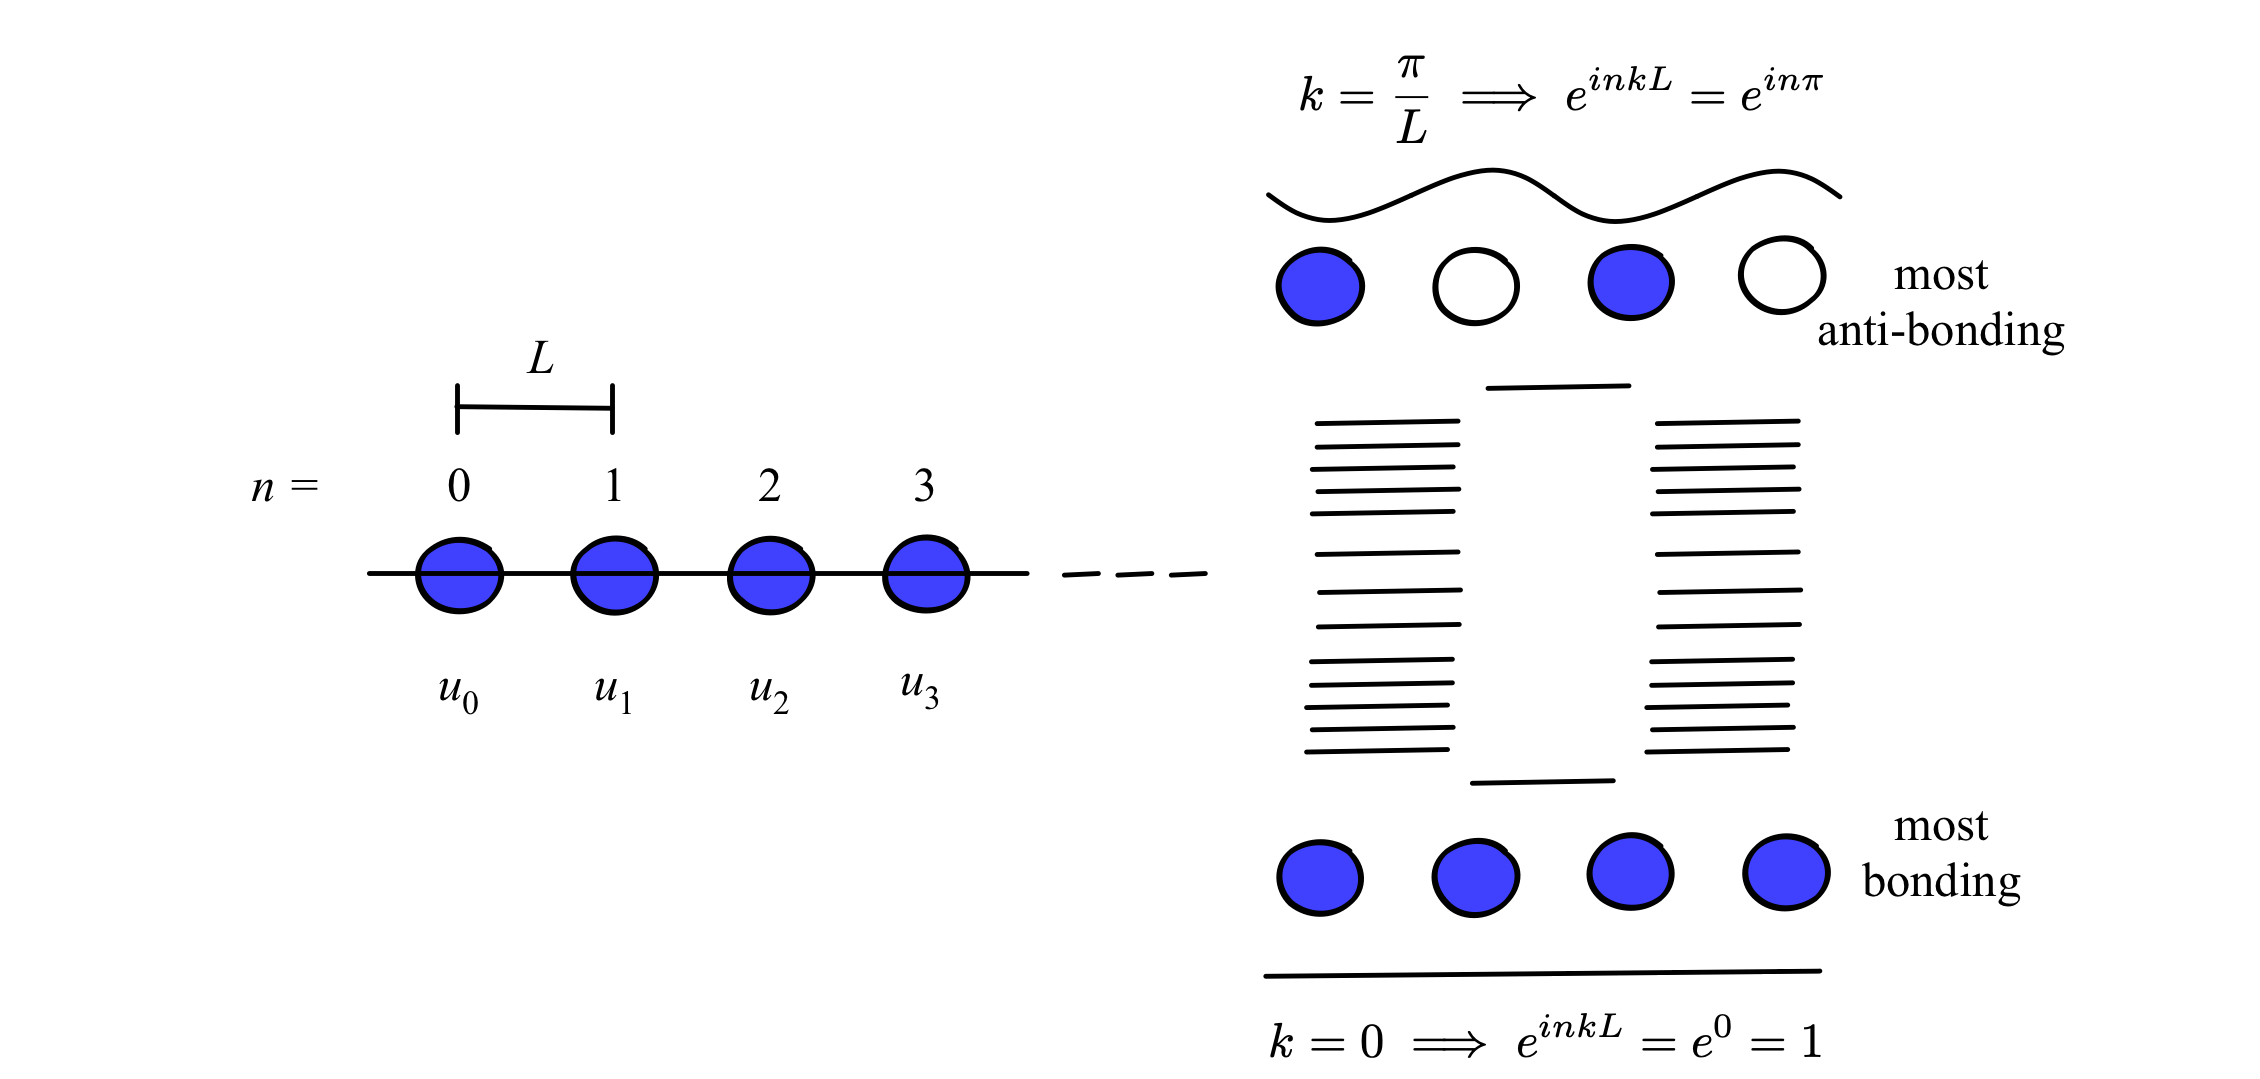
\includegraphics[width=1.0\columnwidth]{figures/ch3/bands.png}
  \caption[Bonding and anti-bonding states in an infinite 1D crystal]{(LHS) A one dimensional infinite lattice where the points are labelled $n=0,1,2\ldots$. The point spacing (unit cell length) is $L$, and there is a hydrogen 1s orbital (basis function) $u_n$ centred at each point. The electron states for this system are formed from Bl\"{o}ch functions as given in Equation \ref{1dbloch}. (RHS) $k=0$ corresponds to a low energy bonding state and $k=\frac{\pi}{L}$ corresponds to a high energy anti-bonding states. Between these two extremes there exists a continuum of states.} 
  \label{bands}
\end{figure}

\subsubsection{Basis Sets}   %valence bands and conductions bands?

In the example of a 1D linear chain, the lattice periodic part of the Bl\"{o}ch function took the form of a hydrogen 1s orbital. For more complex systems, $u_k$ can itself be expanded into a plane wave basis set whose wave vectors $\textbf{G}$ are reciprocal lattice vectors
\begin{equation}
u_\textbf{k} = \sum_\textbf{G}c_{\textbf{k},\textbf{G}}e^{i\textbf{G}\cdot\textbf{r}},
\end{equation}
and the complete expanded Kohn-Sham orbital can be expressed as
\begin{equation} \label{KSeigenstates}
\psi_\textbf{k} = \sum_\textbf{G}c_{\textbf{k},\textbf{G}}e^{i(\textbf{k+G})\cdot\textbf{r}}.
\end{equation}
As a plane wave is inherently periodic this basis set is often used for extended systems. The software used for the DFT calculations in this thesis, \textsc{VASP}\autocite{Kresse1996}, uses a plane wave basis set. For DFT calculations applied to localised systems, such as molecules or nanoparticles, localised basis sets such as gaussian orbitals are more likely to be used.

Sudden changes in electron density are hard to capture using a plane wave basis set; to take an extreme example, the fourier decomposition of a simple top hat in real space requires an infinite summation in reciprocal space. This can be problematic when describing the region around the nucleus where there are strong oscillations in the KS orbitals. However these oscillations are associated with the core electrons which are less important in chemical bonding, and so pseudopotentials - an effective potential without oscillations - can be used. It has been established that for certain systems pseudopotentials are as precise as all-electron calculations.\autocite{Lejaeghere2016}
%http://helper.ipam.ucla.edu/publications/maws3/maws3_6085.pdf
%http://davidbowler.github.io/AtomisticSimulations//blog/dft-reliability#R3

\subsubsection{Optimising the atomic and electronic structure}

In this section the process of optimising the atomic and electronic structure of a system towards the ground-state (minimum energy) configuration is outlined. 

As discussed in Section \ref{DFTtheory}, the potential $v_\textrm{ee}$ is dependent on the electron density $\rho$, which is itself dependent on $v_\textrm{ee}$. Therefore an iterative approach called the Self Consistent Field method is used to calculate the ground-state electronic structure (Figure \ref{SCF}, dashed section). The initial guess for the density $\rho(\textbf{r})$ is given by a superposition of the atomic charge densities. This is used to calculate the potential and solve the KS equations, which gives a new $\rho(\textbf{r})$. This process continues until there is convergence within a given energy tolerance. Various optimisation routines are provided in DFT codes for finding the ground state configuration, including the conjugate gradient scheme, Davidson Scheme and RMM-DIIS.

DFT is also used to find the ground state atomic structure. Structures calculated from X-ray Diffraction data are used as a starting guess, so that finding the energetic minimum becomes a local optimisation problem. Atoms in the systems are displaced (either the internal coordinates of the unit cell or the unit cell parameters themselves are adjusted) and the electronic structure for that geometry is solved self-consistently. This process repeats until the forces on each atom are zero to within a given tolerance (Figure \ref{SCF}). 

\begin{figure}[h]
\centering
  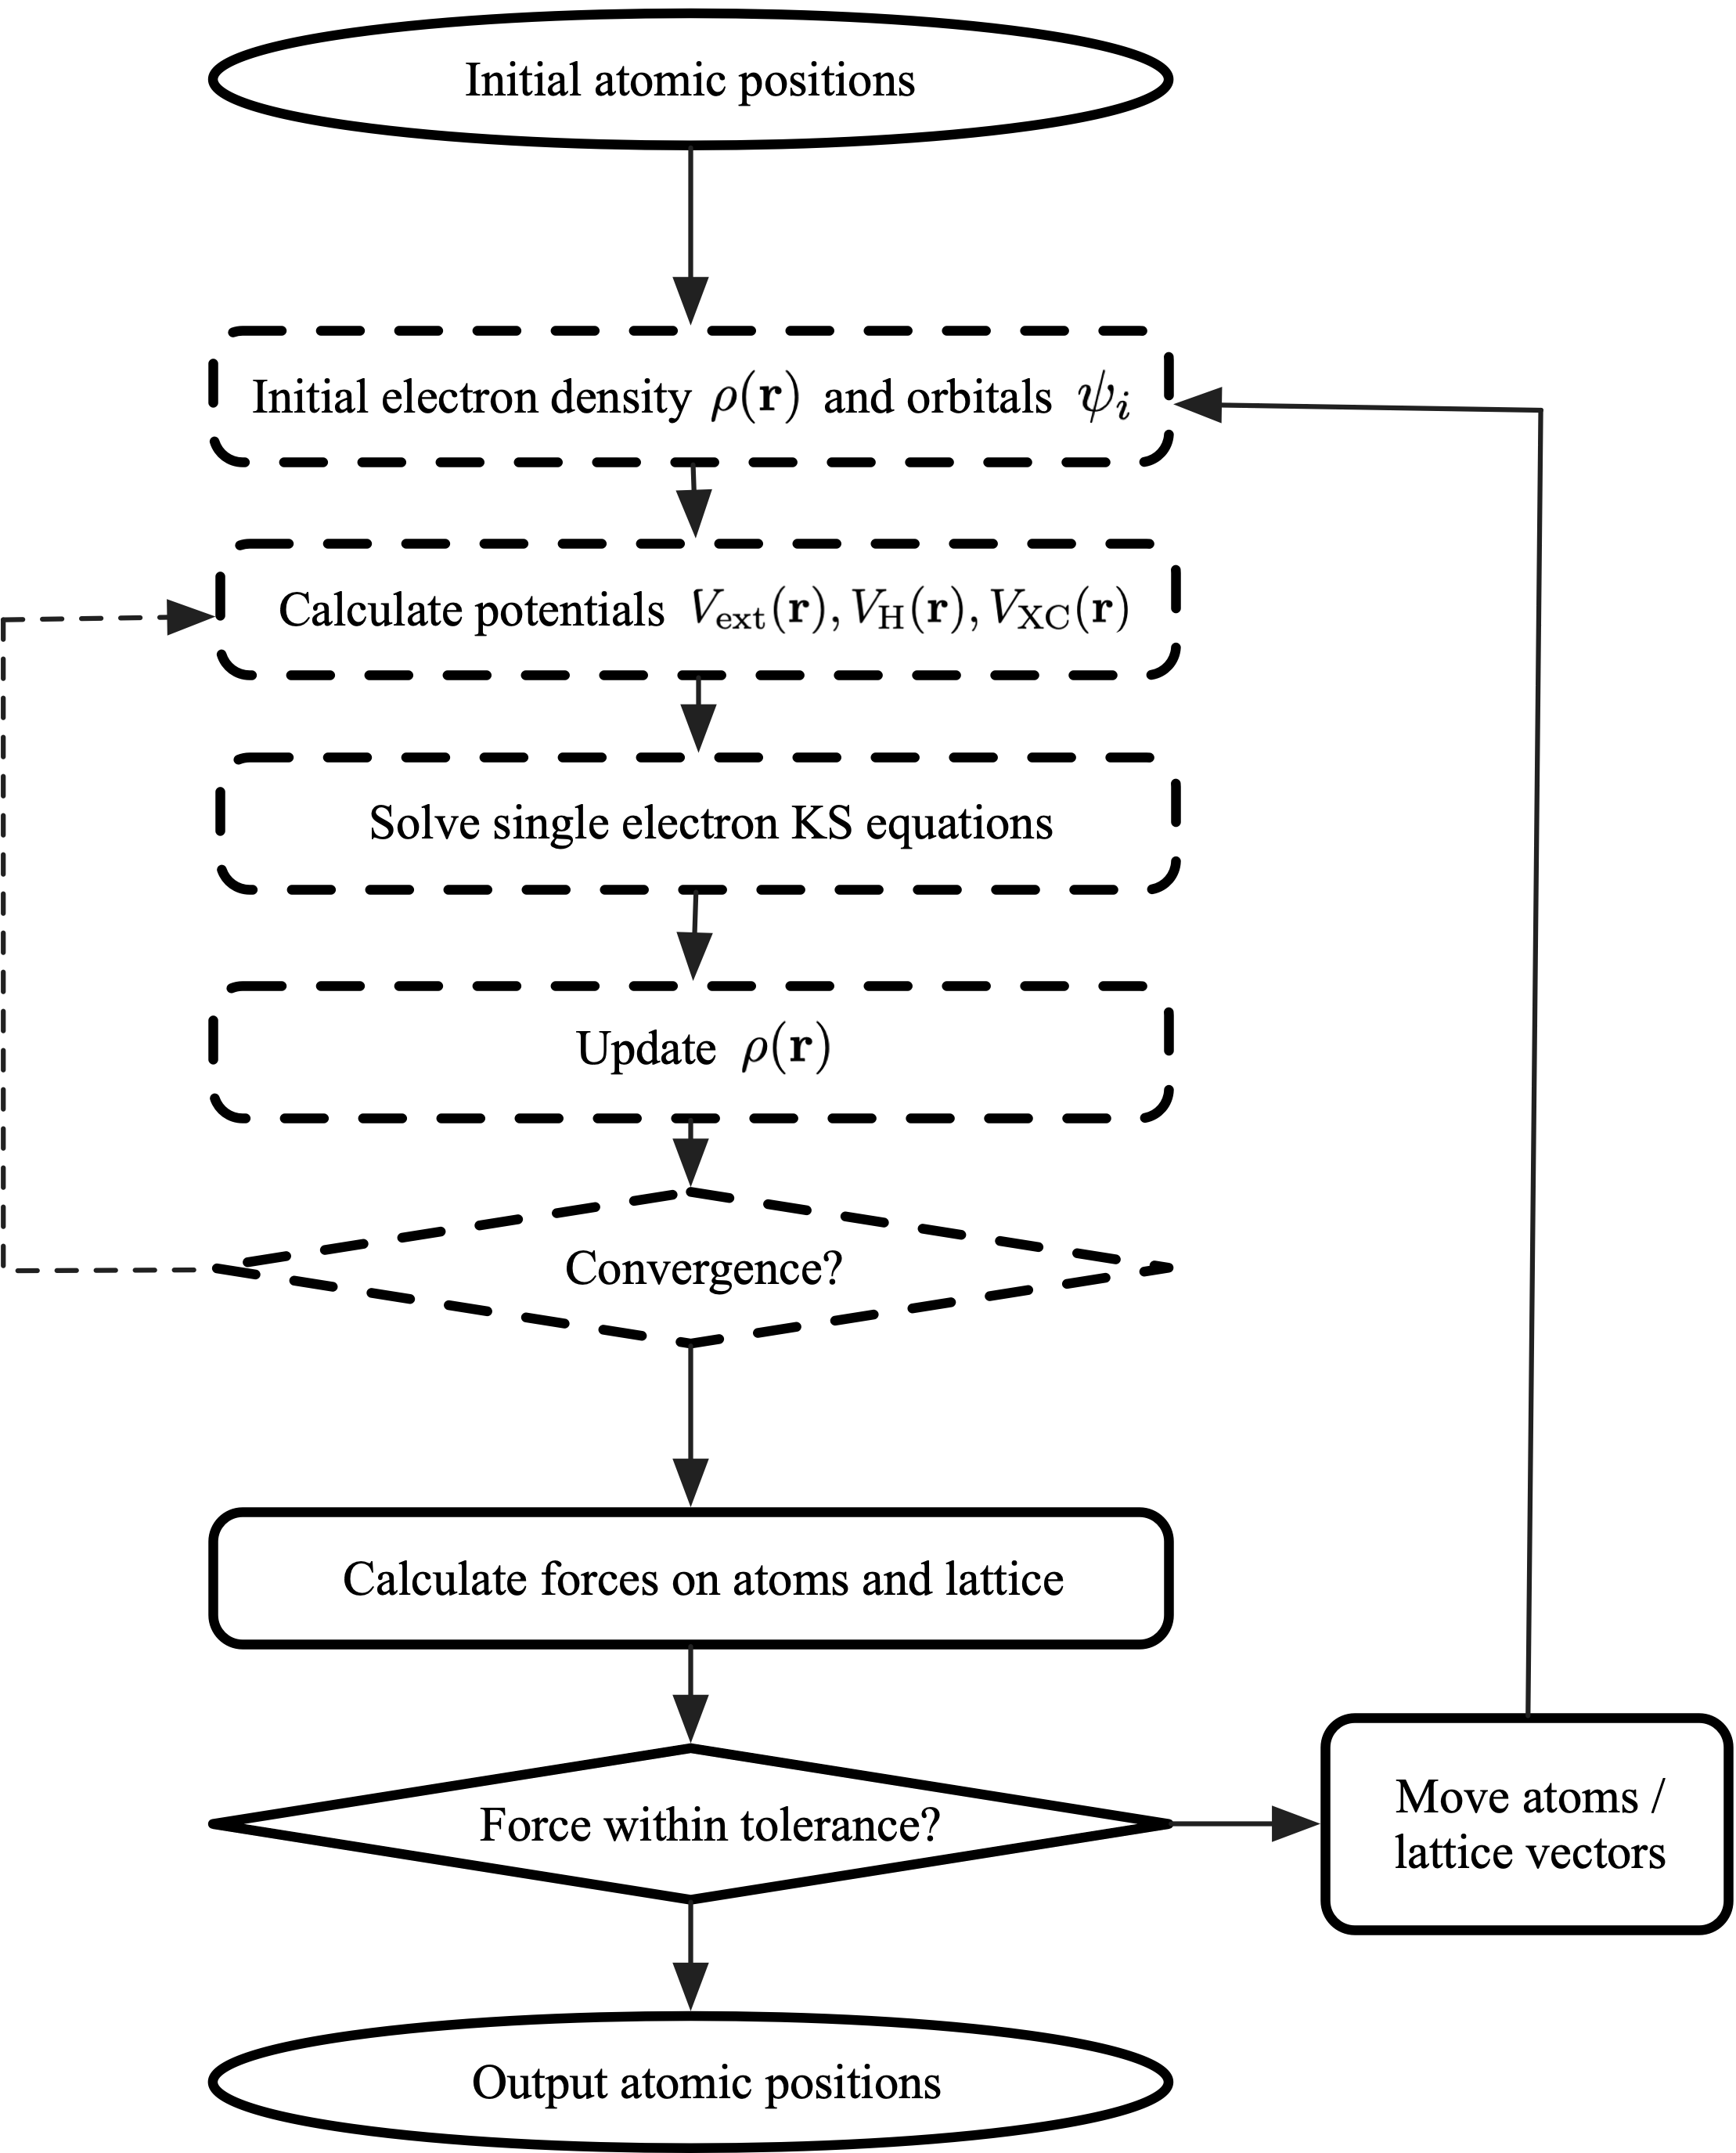
\includegraphics[width=0.7\columnwidth]{figures/ch3/scf.png}
  \caption[Nested iterative method for geometry optimisation]{Nested iterative method for geometry optimisation. The electronic structure relaxation (dashed lines) is nested within the atomic structure relaxation (solid lines). $v_\textrm{ext}(\textbf{r})$, $v_\textrm{c}(\textbf{r})$ and $v_\textrm{xc}(\textbf{r})$ correspond to the external, classical and exchange-correlation potentials respectively.} 
  \label{SCF}
\end{figure}
\subsubsection{The limits of DFT}


\textbf{Theoretical limitations} 

In Section \ref{DFTtheory} the approximations inherent to DFT calculations were outlined: the Born-Oppenheimer approximation and the unknown exchange-correlation functional. Higher levels of theory, which incorporate the effects of spin and relativity (e.g. spin-orbit coupling) are included in many DFT implementations. However DFT is still restricted to ground-state properties and higher levels of theory (GW or time-dependent DFT) are required to describe excited states. Another inherent limitation is that the KS eigenvalues are artificial; only the ground state electron density and derived properties are correct. However in practice the KS eigenvalues are used to calculate the bandgap. Quantitatively correct bandgaps often require the use of hybrid functionals that are parameterised to give the correct bandgap.

\textbf{Numerical limitations} 

There are also approximations that relate to numerical convergence rather than the underlying theory.
We have seen that the KS orbital are expanded in a basis set. In principle an infinite set may be needed to describe the orbitals, but in practice the basis set must be truncated. The kinetic energy operator is given by $-\frac{\hbar \nabla^2}{2m}$ and when this is applied to the plane wave KS orbitals as given in Equation \ref{KSeigenstates}, we find that the kinetic energy is proportional to $|k+G|^2$; faster oscillations correspond to higher energy. A cutoff energy $\textrm{E}_\textrm{cut}$ is defined so that
\begin{equation}
\frac{1}{2}|k+G|^2 < \textrm{E}_\textrm{cut}.
\end{equation}
This cutoff energy must be tested to ensure that the property of interest, most often energy, is converged to within a certain tolerance.

\begin{figure}[h]
\centering
  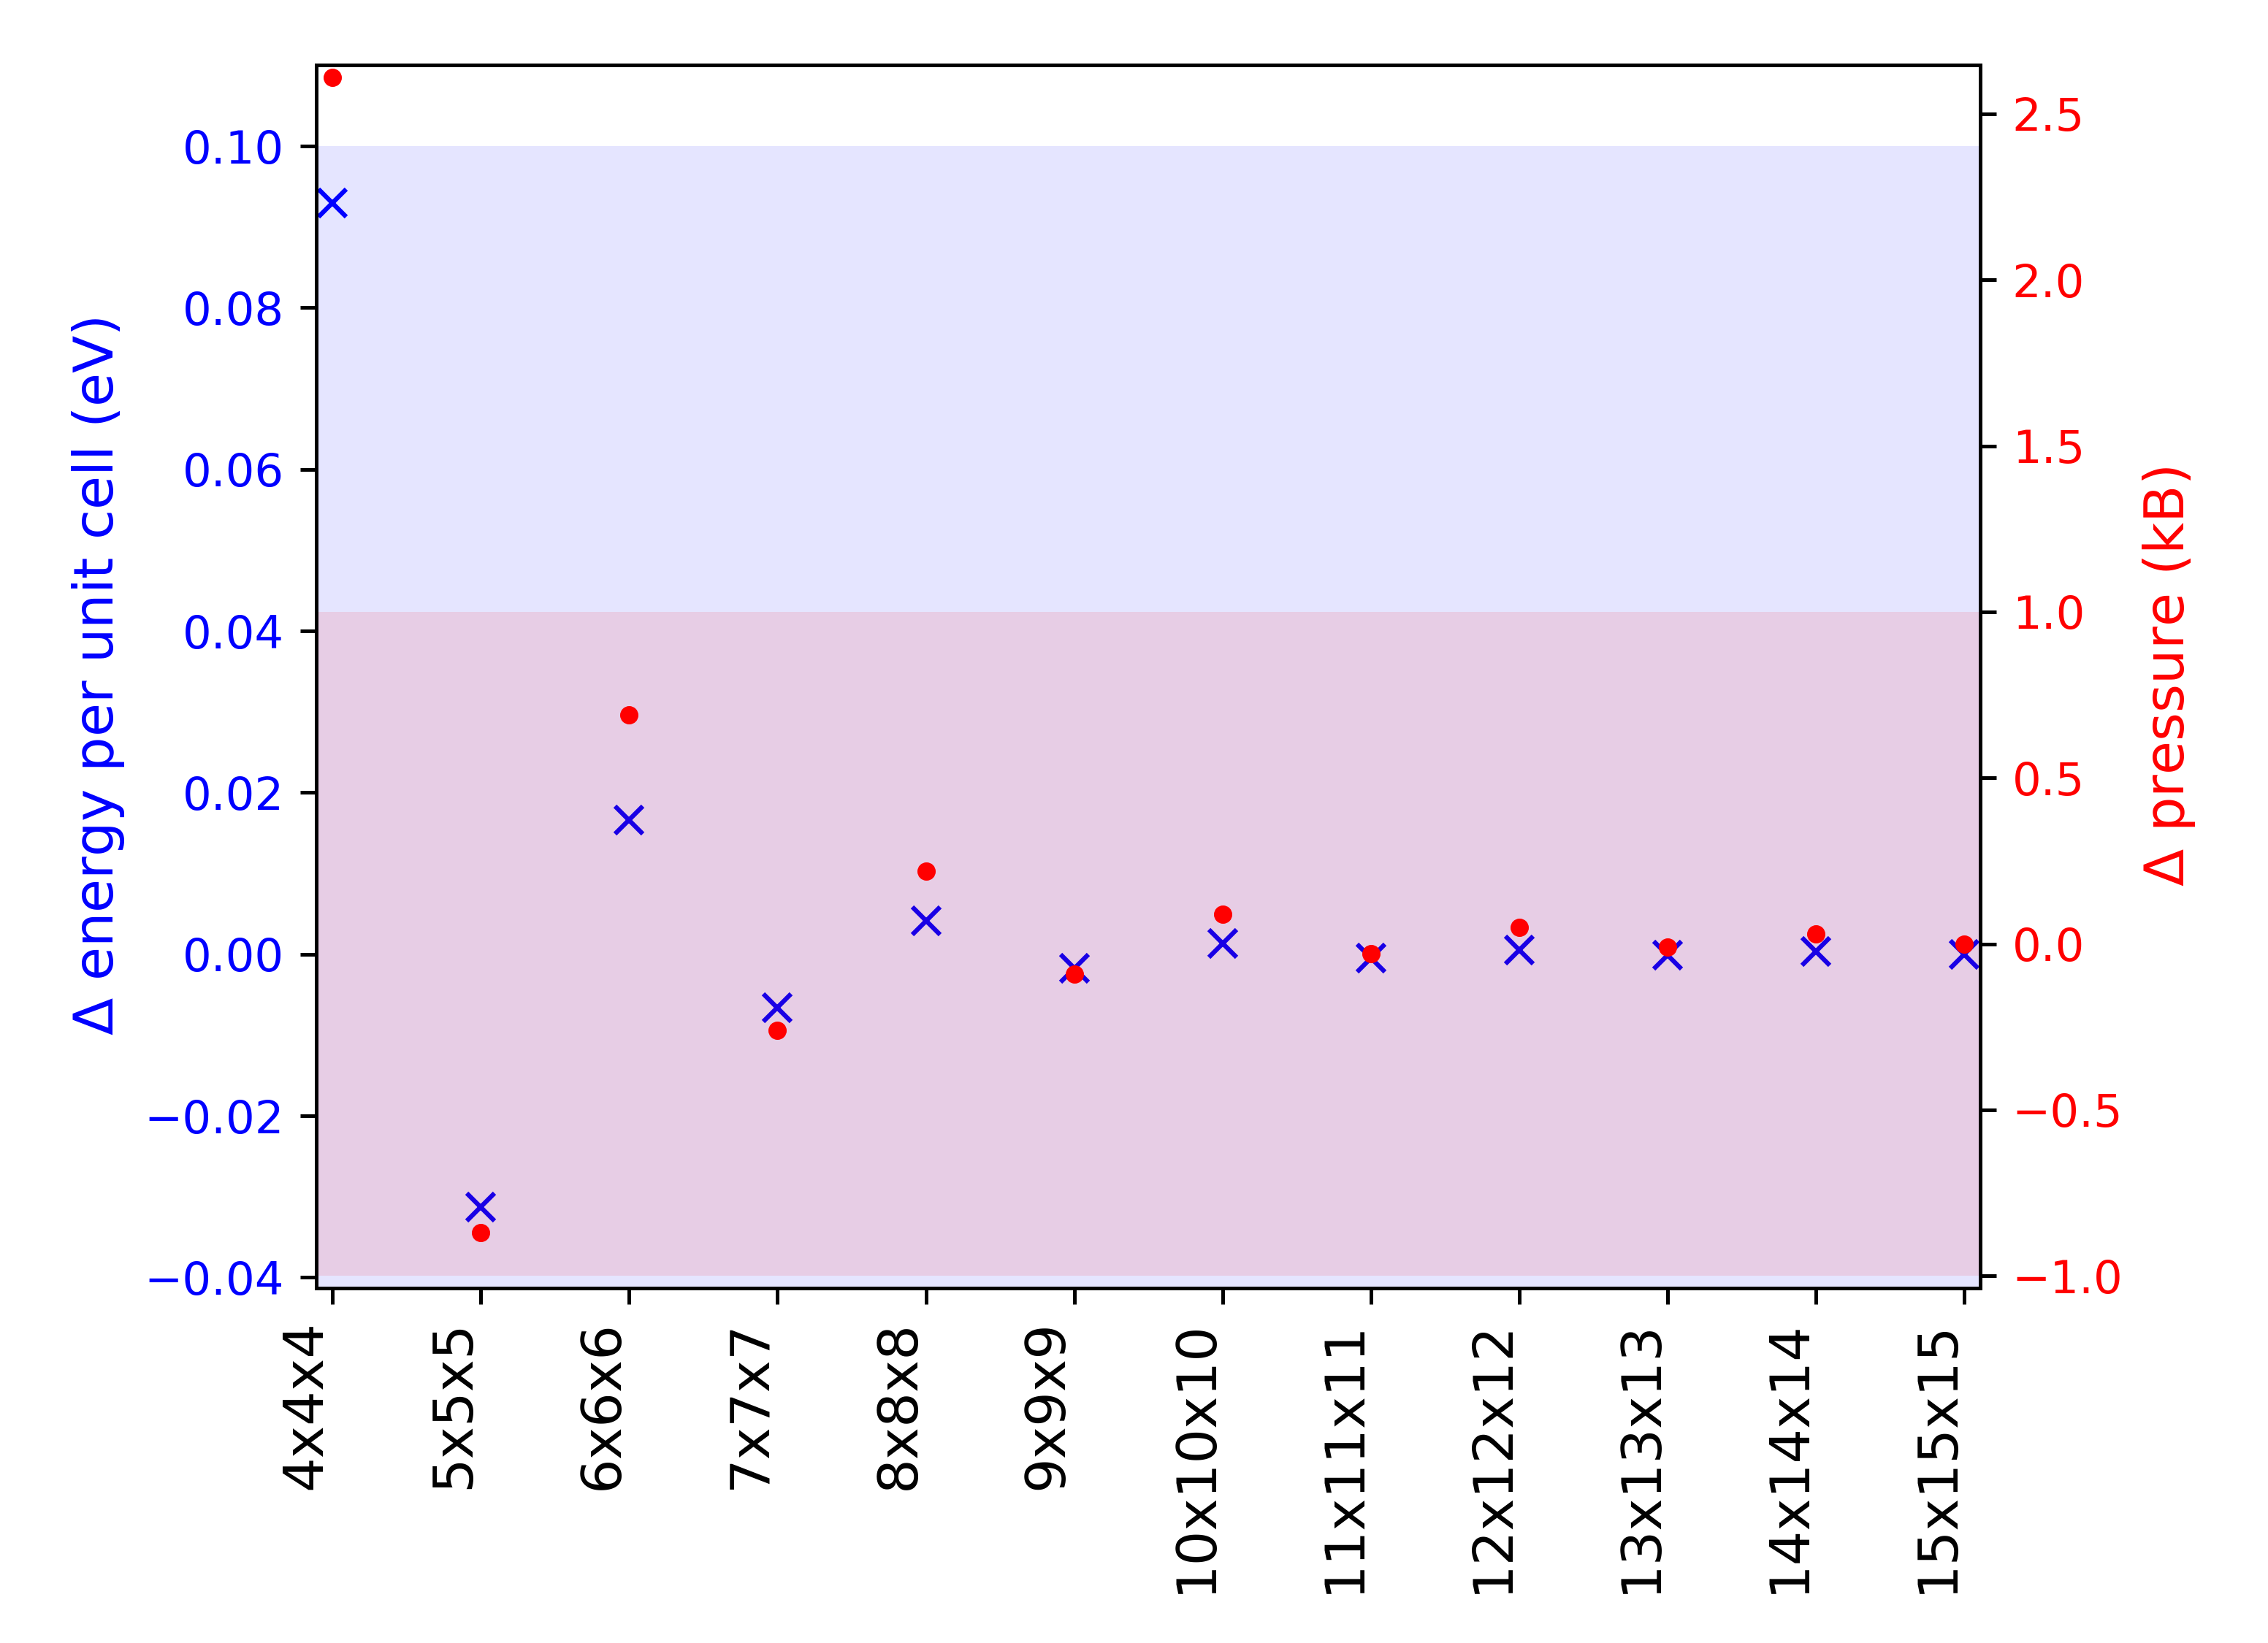
\includegraphics[width=0.7\columnwidth]{figures/ch3/kpointconvergence.png}
  \caption[\ce{CsSnI3} $k$-point convergence]{$k$-point convergence of \ce{CsSnI3}. The $k$-point grid size is on the $x$-axis. Red dots denote pressure; the region which is within the \SI{1}{\kilo\bar} convergence criteria for this study is shaded red. Blue crosses denote total energy; the region which is within the \SI{0.1}{\electronvolt} convergence criteria is shaded in blue. Only odd grids sample the $\Gamma$-point and so there is an oscillation in energy and pressure as points move between odd and even grids.}
  \label{kpointconvergence}
\end{figure}

To calculate many properties of interest we need to integrate over the Brillouin Zone in reciprocal space. To calculate the total energy of an insulator for example, we use
\begin{equation} \label{energyintegral}
    E = \frac{\Omega}{(2\pi)^3}\sum_\textrm{occ.}\int_\textrm{BZ}E(\textbf{k})d^3k
\end{equation}
where $\Omega$ is the volume of the Brillouin zone and the sum is over all occupied bands. 
In practice we do not know the continuous form for $E(\textbf{k})$ and so we numerically evaluate Equation \ref{energyintegral} as a weighted sum over special points in reciprocal space. These points often form an equally spaced mesh centred on the $\Gamma$-point ($\textbf{k}=(0,0,0)$) in reciprocal space. For any given system, the $k$-point density scales inversely with cell size; for example, if the unit cell in Figure \ref{translational} requires a $6\times6$ $k$-point grid, then the larger $2\times2$ supercell requires a $3\times3$ $k$-point grid. As with plane waves, there is a balance between accuracy (the higher the number of $k$-points, the higher the accuracy) and computational expense. An example convergence study is given in Figure \ref{kpointconvergence} where a $5\times5\times5$ $k$-point grid is required to converge pressure to within \SI{1}{\kilo\bar} and energy to within \SI{0.1}{\electronvolt} in \ce{CsSnI3}.


% - K-point grids and the commensurate grids for supercells.
% - Doubles k-points reuired as k and –k now no longer equivalent (SoC?)
%All convergence tests must be done for the property of interest. Cancellation of errors can mean that energy differences converge faster than ground state energies, as is reported in Chapter \ref{}.   % EP coupling calcas 
% - See: Designing meaningful density functional theory calculation in materials science - a primer Anne E Mattson et al. Model. Sim. Mater. Sci Eng. 13 R1-R31 (2005). : for information about convergence and getting meaningful results.

%\textit{Computational limitations}
% - history of computers section at science museum for HPC section
% - put the amount of computer time and carbon burnt here?
% - computational expense: limitations on size: See review of materials models which Alison Walker mentions. Mesoscopic bridges the atomistic with the drift diffusion models. Meso is often monte carlo, tranjectory tpe calculations. Cells are too big for atomistic (1 cm squared). Efficiecny depends upon J-V curves which can only be modelled at scale of fill device. The electrostatics is incredible important which linked ot build up of charges at SC nd OC. Grain boundaries and recombination at intercaes.

\section{Defects in semiconductors}

The second law of thermodynamics states that an isolated system tends towards an equilibrium state with maximum entropy. A consequence of this is that all solids in equilibrium and at finite temperature contain point defects, as the cost in lattice energy is balanced by the increase in configurational entropy. 
Point defects are associated with a number of microscopic processes that can be either beneficial or detrimental to material performance, including:
\setlist{nolistsep}
\begin{itemize}[noitemsep]
    \item optical: colour centres, up/down conversion
    \item electrical: conductivity, carrier trapping, ionic hopping
    \item mechanical: material hardening
    \item thermal: conductivity, decomposition
\end{itemize}
%Yakov Frenkel introduced the concept of defects in a crystalline structure in 1926. Research interest in this field continued throughout the 20th and 21st centuries as the physical processes listed above determine the success or failure of technologically important materials. 
Theoretical methods are particularly useful in this area as although it is often possible to estimate the quantity of defects in a material using experimental methods, it is much more challenging to identify the defect species.\autocite{Alkauskas2016}  
 
In this section I outline the different types of crystal defects and discuss the thermodynamics of (charged) defect formation. The supercell method for calculating defect properties is also outlined. This method is used in Chapter \ref{ch:6-defects}.
% We are interested in calculating the electronic structure properties which lead to a description of the defects (trap density, binding energy, trap level, capture cross section).

% cite defects and defect processes in nonmetallic solids

% - History:
% - 1912 Born and Karman . PBC (first lattice dynamics paper)
% - 1925 Frenkel – formation of frenkel pair (first defects paper)
% - 1922 Jost – probability of forming defects. Tied into experimental work popular at the time, looking at how a material can be an ionic conductor when it is electrically insulating
% - 1938 Mott – the Mott-Littleton approach for calculating defects

\subsection{Classification of crystal defects}

The first way to classify defects is via their dimensionality. 0-dimensional point defects are localised around isolated sites in the crystal. 1-dimensional dislocations are lines along which the crystal pattern is broken. 2-dimensional grain boundaries or interfaces are surfaces along which distinct crystallites are joined. 3-dimensional defects are changes to the crystal pattern in a finite volume. 

0-dimensional point defects are the subject of Chapter \ref{ch:6-defects}. Point defects can be further split into extrinsic or intrinsic defects. Extrinsic point defects (also known as impurities) are a different species from that of the host. These defects may be added intentionally (for example, to increase electrical conductivity) or unintentionally (as a result of the fabrication method). Intrinsic point defects are associated with the host species.

Point defects can also be classified as non-stochiometric or stochiometric. Non-stochiometric defects include interstitials (where an additional atom occupies a site that is unoccupied in the perfect lattice), vacancies (missing atoms) and antisites (where an atom occupies a site that would have been occupied by another species in the perfect lattice). Interstitials can have a `split' structure, in which two atoms are split symmetrically around a single lattice site. Stochiometric defects include Frenkel pairs and Shottky pairs. Stochiometric and non-stochiometric point defects are illustrated in Figure \ref{classification}.

\begin{figure}[h]
\centering
  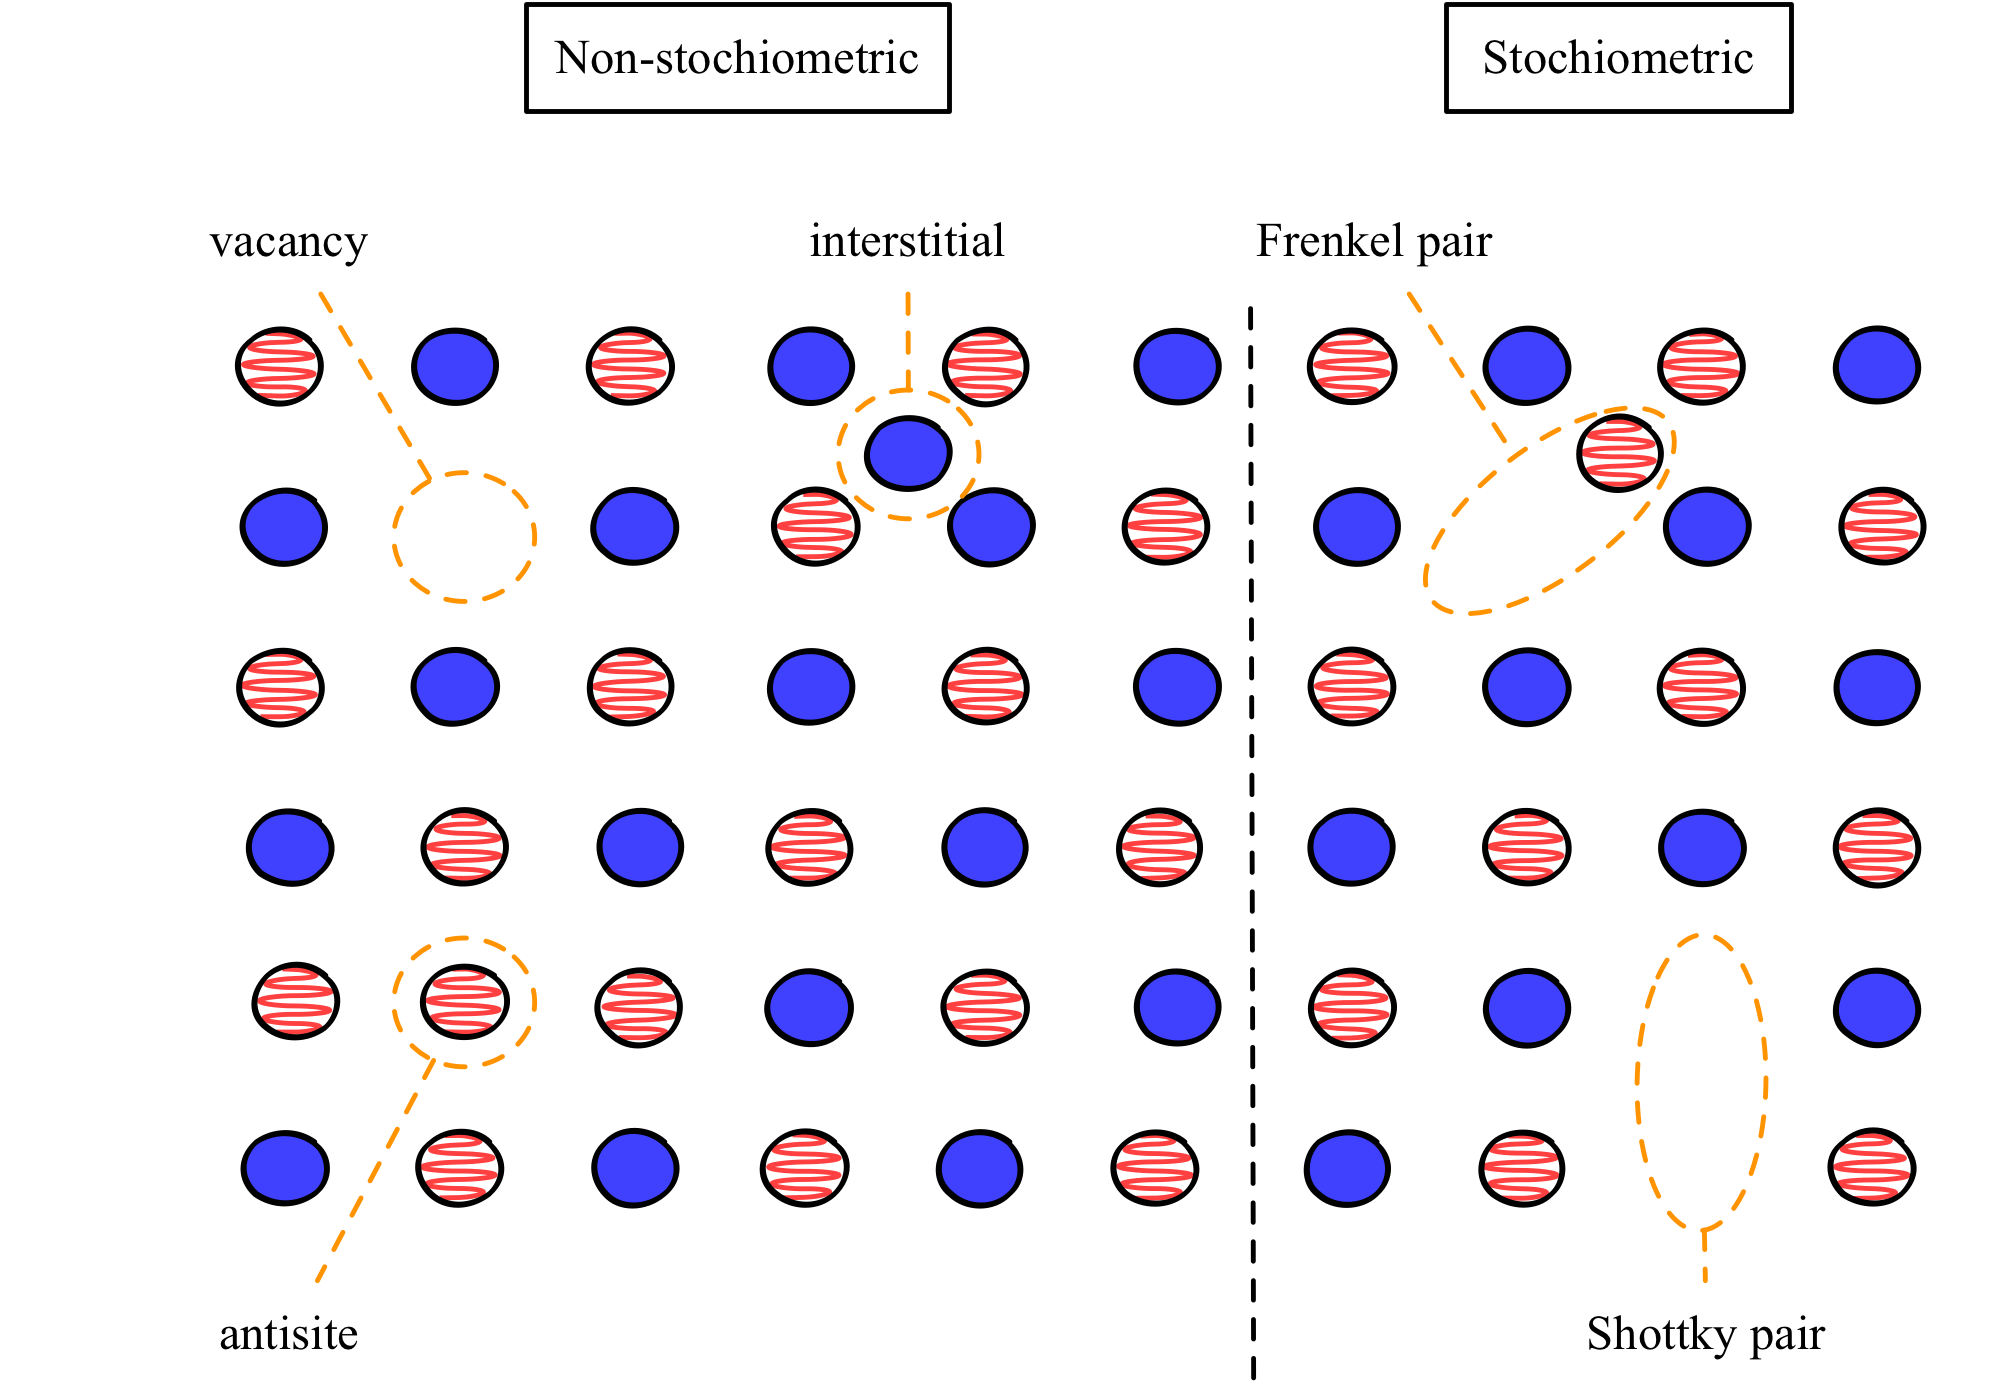
\includegraphics[width=0.8\columnwidth]{figures/ch3/classification.png}
  \caption[Classification of crystal point-defects]{Non-stochiometric defects include interstitials (an additional atom), vacancies (a missing atom) and anti-sites. Stochiometric defects include a Frenkel pair (a vacancy close to an interstitial of the same species), and a Shottky pair (a vacancy on both the anion and cation sub-lattices).}
  \label{classification} . %hatch the shapes in this drawing so can tell the differene in b+w
\end{figure}

The final classification is into electrically active and electrically benign defects. Whilst electrically benign defects exist only in one charge state, electrically active defects can take more than one charge state; for example, single acceptors exist in a neutral or negatively charged state and single donors exist in a neutral or positively charged states. Amphoteric defects can exist in a negatively charged or positively charged state.
% reference alkasukas https://www.osti.gov/pages/servlets/purl/1471061
% - may be able to say defect is there experimentally but another step to identify which it is. Admittance spectroscopy, DLTS. ESR (later chapter)
% emphasise that the concentration could be as low as one part in a milllion and wtill have an effect.
% - defect levels deend on temperature. DLTS assumes T-independent scattering cross sction, not accurate,

\subsection{Energetics of defect formation} \label{defectformation}

The equilibrium concentration of defects $n$ at a fixed temperature and pressure is given by the density that minimizes free energy.
\begin{equation} \label{defectconcentration}
    n = N_\mathrm{sites} \exp \left(-\frac{\Delta G}{k_\mathrm{B} \mathrm{T}} \right),
\end{equation}
where $\Delta G$ is the Gibbs free energy of defect formation. The Gibbs free energy is approximated as the formation energy $E_\mathrm{f}$ of the defect as this dominates over entropic contributions. The formation energy is given by:
\begin{equation} \label{eqn_formation_energy}
E_\mathrm{f}(q) = E_\mathrm{d}(q) - E_\mathrm{b} - \sum_i \mu_i n_i + q(\epsilon_\mathrm{VBM}+E_\mathrm{F}) + E_\mathrm{corr},
\end{equation}
where $E_\mathrm{d}(q)$ is the total energy of the supercell with a defect of charge $q$ and $E_\mathrm{b}$ is the total energy of the perfect bulk. 
$E_\mathrm{corr}$ is a correction energy that is only needed for charged defects and is discussed Section \ref{corrections}.
The remaining terms describe the energy needed to add or remove atoms or electrons.
$\mu_i$ is the chemical potential of atom $i$ and $n_i$ is the number of atoms that are added or removed.
The chemical potential can be adjusted to describe different growth conditions; if the growth conditions are rich for species $i$ then $\mu_i$ will be low.
$E_F$ is the Fermi level of the electrons, referenced to the valence band maximum $\epsilon_\mathrm{VBM}$.

The total energies can be calculated using DFT. Convergence criteria for calculations must be tight as, due to the exponential dependence of defect concentration on formation energy, small errors in the energy difference can lead to large errors in the defect concentration.

The Fermi level is treated as a parameter, of which the defect formation energy is a linear function with a gradient equal to the defect charge. This allows us to plot a graph of formation energy against Fermi level, as shown in Figure \ref{CdTeformation}. Charge transition levels mark the Fermi level at which two charge states have the same defect formation energy. Electrically active defects have at least one charge transition level in the bandgap. 
The charge transition level is equivalent to thermal ionization energy, the energy needed to add or remove electron(s). % check this
% does not always need a charge transition level deep in the bandgap. https://pubs.acs.org/doi/pdf/10.1021/acsenergylett.7b01313

\begin{figure}[h]
\centering
  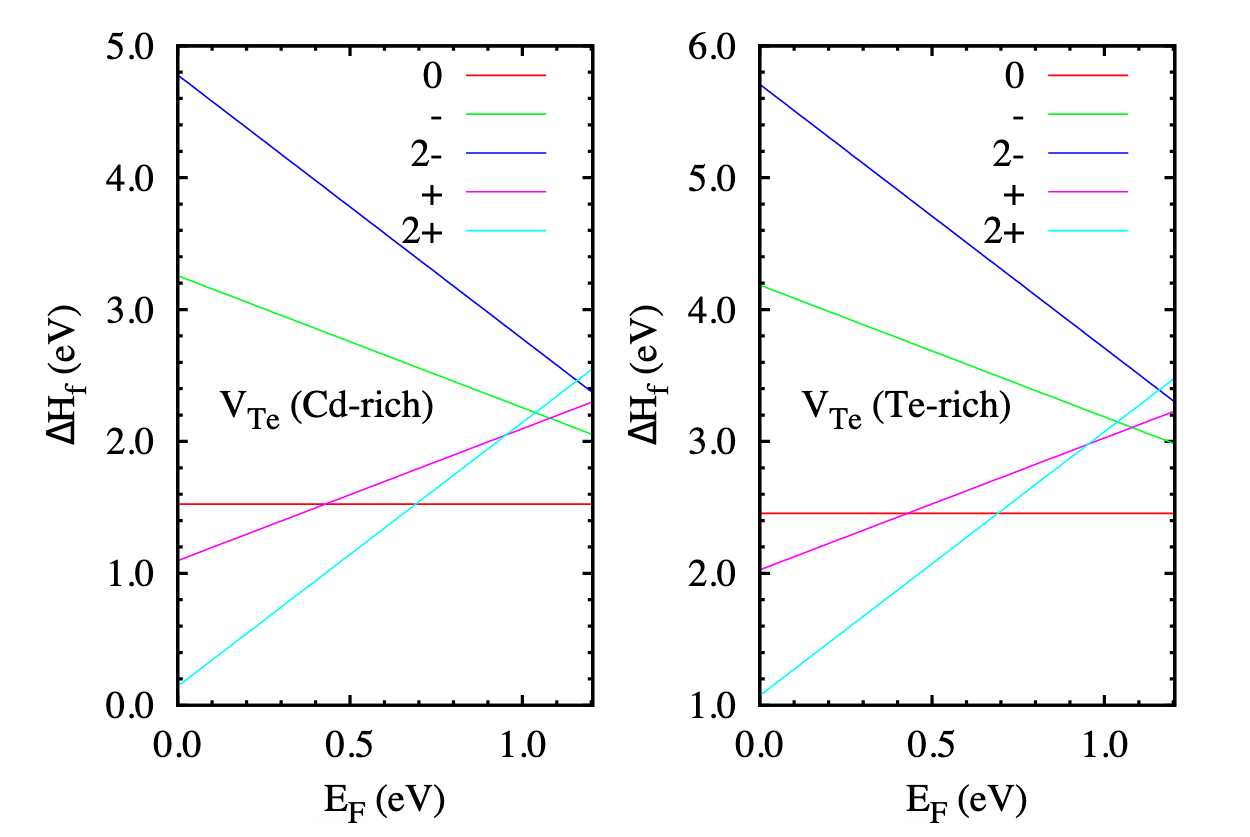
\includegraphics[width=0.8\columnwidth]{figures/ch3/defectenergetics.png}
  \caption[Formation energies of the Te vacancy in CdTe]{Formation energies $\Delta H_f$ as a function of the Fermi energy for the Te vacancy in \ce{CdTe}. In a Te-rich environment it is more energetically unfavourable to form a Te-vacancy, as intuition would suggest. The slope of each line corresponds to the defect charge. Charge transition levels correspond to the energies at which the lines intersect. Figure reproduced with permission from the work of Menendez et al.\autocite{Menendez2016}}
  \label{CdTeformation}
\end{figure}%cite https://iopscience.iop.org/article/10.1088/1742-6596/720/1/012031/pdf

Defect levels deep in the bandgap correspond to localised wavefunctions. Carrier capture processes to these defect states are often associated with a large lattice distortion. Shallow defect levels (within thermal energy $k_BT$ of the valence or conduction band) correspond to delocalised, hydrogenic-like defect wavefunctions. 
% - defect energies theoretical founsations - mott littleton (1938)  - a way to calculate E the defecct energy as knew the hopping rate expression, but didnt know E. only experimental input is dielectric constant.see special 1988 issue.
%  The other problem is that is dependent upon the chemical potential which is difficult to monitor.

% Point defects result in additional energy levels in the bandgap with an associated defect wavefunction to which an electron is added or removed.
% defect level delocalised, electrical conductivity.EMT.
%or deep and localised wavefucntion. detrimental in the context of solar cells.

%The concentration of a point defect in a particular charge state can be controlled by tuning the Fermi level through doping. However there is a compensation mechanism, whereby defects form to compensate

% The concentration of point defects can be controlled by thermal treatment, irradiation or doping. 
% - Fermi level pinning (?) / defect concentration: Happens in TCO’s such as FTO. Above a certain concentration there are no more holes. This could happen when there are defect complexes which compensate each other.
% - This is a compensation mechanism. We try to adjust the fermi level of the system by introducing impurities. However above/below a certain energy level there is spontaneous formation of defects (defects which have a negative energy of formation). These defects compensate for the impurity and in this way the fermi level is pinned.

% - Calculable and observable table:
% Delta E : heat of formation / concentrations
% Defect ionisation – optical – instanataneour: PL, optical absorption / photoconductivity
% Defect ionisation , thermal, after relaxation: DLTS / thermally stimuated conductuvtiy
% Defect vibrational modes: IR/raman spectra and recombination rates

\subsection{Supercell method}

Defect concentrations as low as one part in one million can have an influence on device performance. 
One way to model point defects in the dilute limit, when defect-defect interactions are negligible, is to build a supercell from multiple unit cells (Figure \ref{translational}).
This supercell must be large enough so that there is no interaction between a defect and its periodic images.
Although the supercell method captures localised defects well, it cannot capture the behaviour of delocalised (or band resonant) defects due to the enforced periodicty. 
%http://cmt.dur.ac.uk/sjc/thesis/thesis/node71.html
To remove the constraint of translational symmetry it is possible to use an embedded QM/MM approach whereby a region around the defect is modelled using DFT and embedded in a region that is modelled classically.

% - The supercell method leads to some unphysical results for both electronic and vibrational properties. The defect will perturb the lattice. The SC method captures localised defect effects well – but the delocalised defects (possibly in the band) are not captured as there is an enforced periodicity. The only way around this is to use greens functions method (phonons) or QM/MM approach (electrons).
% vibrations of defects - link to final chapter

\subsubsection{Supercell corrections} \label{corrections}
% this is from the joint JPhysChem defects review paper - if its published I will need to cite it!
% previous section - defect-defect interaction but there are also longer ranged coloumb interations
Point defects can be electrically charged, and are able to change charge state through the trapping and de-trapping of electrons and holes. 
The charge state of a defect can affect a number of defect properties including the preferred lattice position, surrounding lattice distortion, and the rates of diffusion, carrier capture, and carrier recombination.
However, due to the long range nature of the Coulomb interaction, understanding the properties of charged defects is a challenge for DFT with periodic boundary conditions.
There are two issues to resolve: 
Firstly, charged defects can interact with their periodic images; 
Secondly, a homogeneous `jellium' background charge is introduced to ensure overall charge neutrality and results in an unknown shift to the average electrostatic potential. 
These are finite-size effects that only a very large, almost infinite, supercell would overcome.
However a system this size is computationally intractable, especially considering that higher levels of theory (for example, hybrid functionals) are often required to calculate accurate total energies.

A number of correction schemes have been developed to deal with these issues; a brief historical overview is given below. These schemes are designed to be used as a post-processing step and provide a value for the $E_{corr}$ term in Eqn.\ref{eqn_formation_energy}. A more complete description of these issues can be found in References \cite{durrant2018} and \cite{Vinichenko2017}.

The Leslie Gillan correction\autocite{Leslie1985} $E^\mathrm{LG}$ models the defect charge $q$ as a point charge interacting with its periodic images through an isotropic dielectric medium. 
This correction takes a simple analytic form that depends on the charge state  $q$, static dielectric constant $\epsilon_0$, separation between defect images $L$ and the Madelung constant $\alpha_m$, which is determined by the lattice geometry:
\begin{equation}
    E^\mathrm{LG} = \frac{q^2\alpha_{m}}{2\epsilon L}.
\end{equation}
The Markov-Payne correction $E^\mathrm{MP}$ extends the Leslie Gillan correction by including an additional term that accounts for the delocalised part of the defect charge. 
\begin{equation}
    E^\mathrm{MP} = \frac{q^2\alpha_{m}}{2\epsilon L} + qQL^{-3}. 
\end{equation}
The challenge of the Markov-Payne approach is in calculating the quadrupole moment $Q$. 
The Lany-Zunger correction\autocite{Lany2009} combines the Markov-Payne correction, including an approach for calculating $Q$, with a potential alignment procedure to correct for the shift in electrostatic potential. 
The Freysholdt, Neugebauer and van de Walle (FNV) method\autocite{Freysoldt2009} models the defect charge as a localised gaussian distribution. 
The difference between the electrostatic potential of the charged defect supercell and the electrostatic potential of the perfect bulk supercell, calculated far from the defect, is aligned with the defect model potential. 
Kumagai and Oba have extended to FNV method by using atomic site potentials combined with a point charge model for an anisotropic medium.\autocite{Kumagai2014} 

There is still no standardised approach to defect charge corrections, 
which can lead to a spread in calculated defect formation energies in the literature, and predicted defect densities which differ by orders of magnitude.
Two widely used approaches in the recent literature are the FNV method, and the extension to this provided by Kumagai and Oba.
This extension is applied to the iodine interstitial defect in Chapter \ref{ch:6-defects}, using an implementation in the package \textsc{sxdefectalign}.
% - for a really good explanation see Suzys group talk (Monday the 10th september 2018) and https://aip.scitation.org/doi/10.1063/1.5029818 which it was based upon.
%what are the corections used in this work?


\section{Lattice dynamics} \label{sec:latticedynamics}
%cite defect and defect processes in nonmetallic solids
%cite Dove Lattice dynamics
This section includes a brief overview of the theory of lattice dynamics, with a particular focus on anharmonic atomic motion. The finite difference method, an intuitive way to calculate the vibrational properties of a crystal, is outlined. This method has been applied to the perfect bulk in Chapter \ref{ch:5-epcoupling} and a defect supercell in Chapter \ref{ch:6-defects}.

Heisenberg's uncertainty principle states that it is not possible to know both the position and momentum of a particle exactly. Thus the static lattice model used so far is only an approximation; even at $T=0\,\textrm{K}$ there is zero point atomic motion. As temperature increases, this vibrational motion increases in amplitude.

The lattice vibrations of a crystal must be considered to calculate a number of physical properties. Atomic motion has an associated vibrational energy, and this determines crystal stability as a function of temperature via the Gibbs free energy:
\begin{equation}
G = E_0+E_\textrm{vib}+PV-TS
\end{equation}
where $E_0$ is the ground state energy, which can be calculated using DFT, and $E_\textrm{vib}$ is the vibrational contribution to internal enery.
Atomic motion also influences the electrical and optical properties of a crystal; this can be seen experimentally in the homogeneous broadening of photoluminescence linewidths with temperature, for example.\autocite{silsbee1962}%cite https://journals.aps.org/pr/abstract/10.1103/PhysRev.128.1726
Other material properties which are only accessible via lattice dynamics include: heat capacity, thermal conductivity, elasticity, thermal expansion coefficients, electron-phonon coupling strengths and static polarization.

For atomic motion at small amplitudes around the potential energy minimum it is common to use the harmonic approximation, where the atom moves as if it is connected by a spring to its neighbouring atoms (Figure \ref{harmonicregime}). This is discussed in Section \ref{harmonicapprox}. At larger vibration amplitudes, and to understand processes relating to the creation and annihilation of phonons, we must consider anharmonic motion, and this is considered in Section \ref{anharmonicapprox}.

These motions are determined by the force on each atom. For simple systems, for example a one-dimensional diatomic chain, we can calculate atomic position as a function of time analytically. Otherwise methods such as DFT can be used to build a force constant matrix which, after some post-processing steps, gives the eigenvectors (direction) and frequencies of motion. This is discussed in Section \ref{finitedisplacement}. As in the previous sections of this chapter, we use the Born-Oppenheimer approximation and assume that the equilibrium positions in a crystal are the minima of the potential energy surface when the electron and nuclear motion are decoupled.

\begin{figure}[h]
\centering
  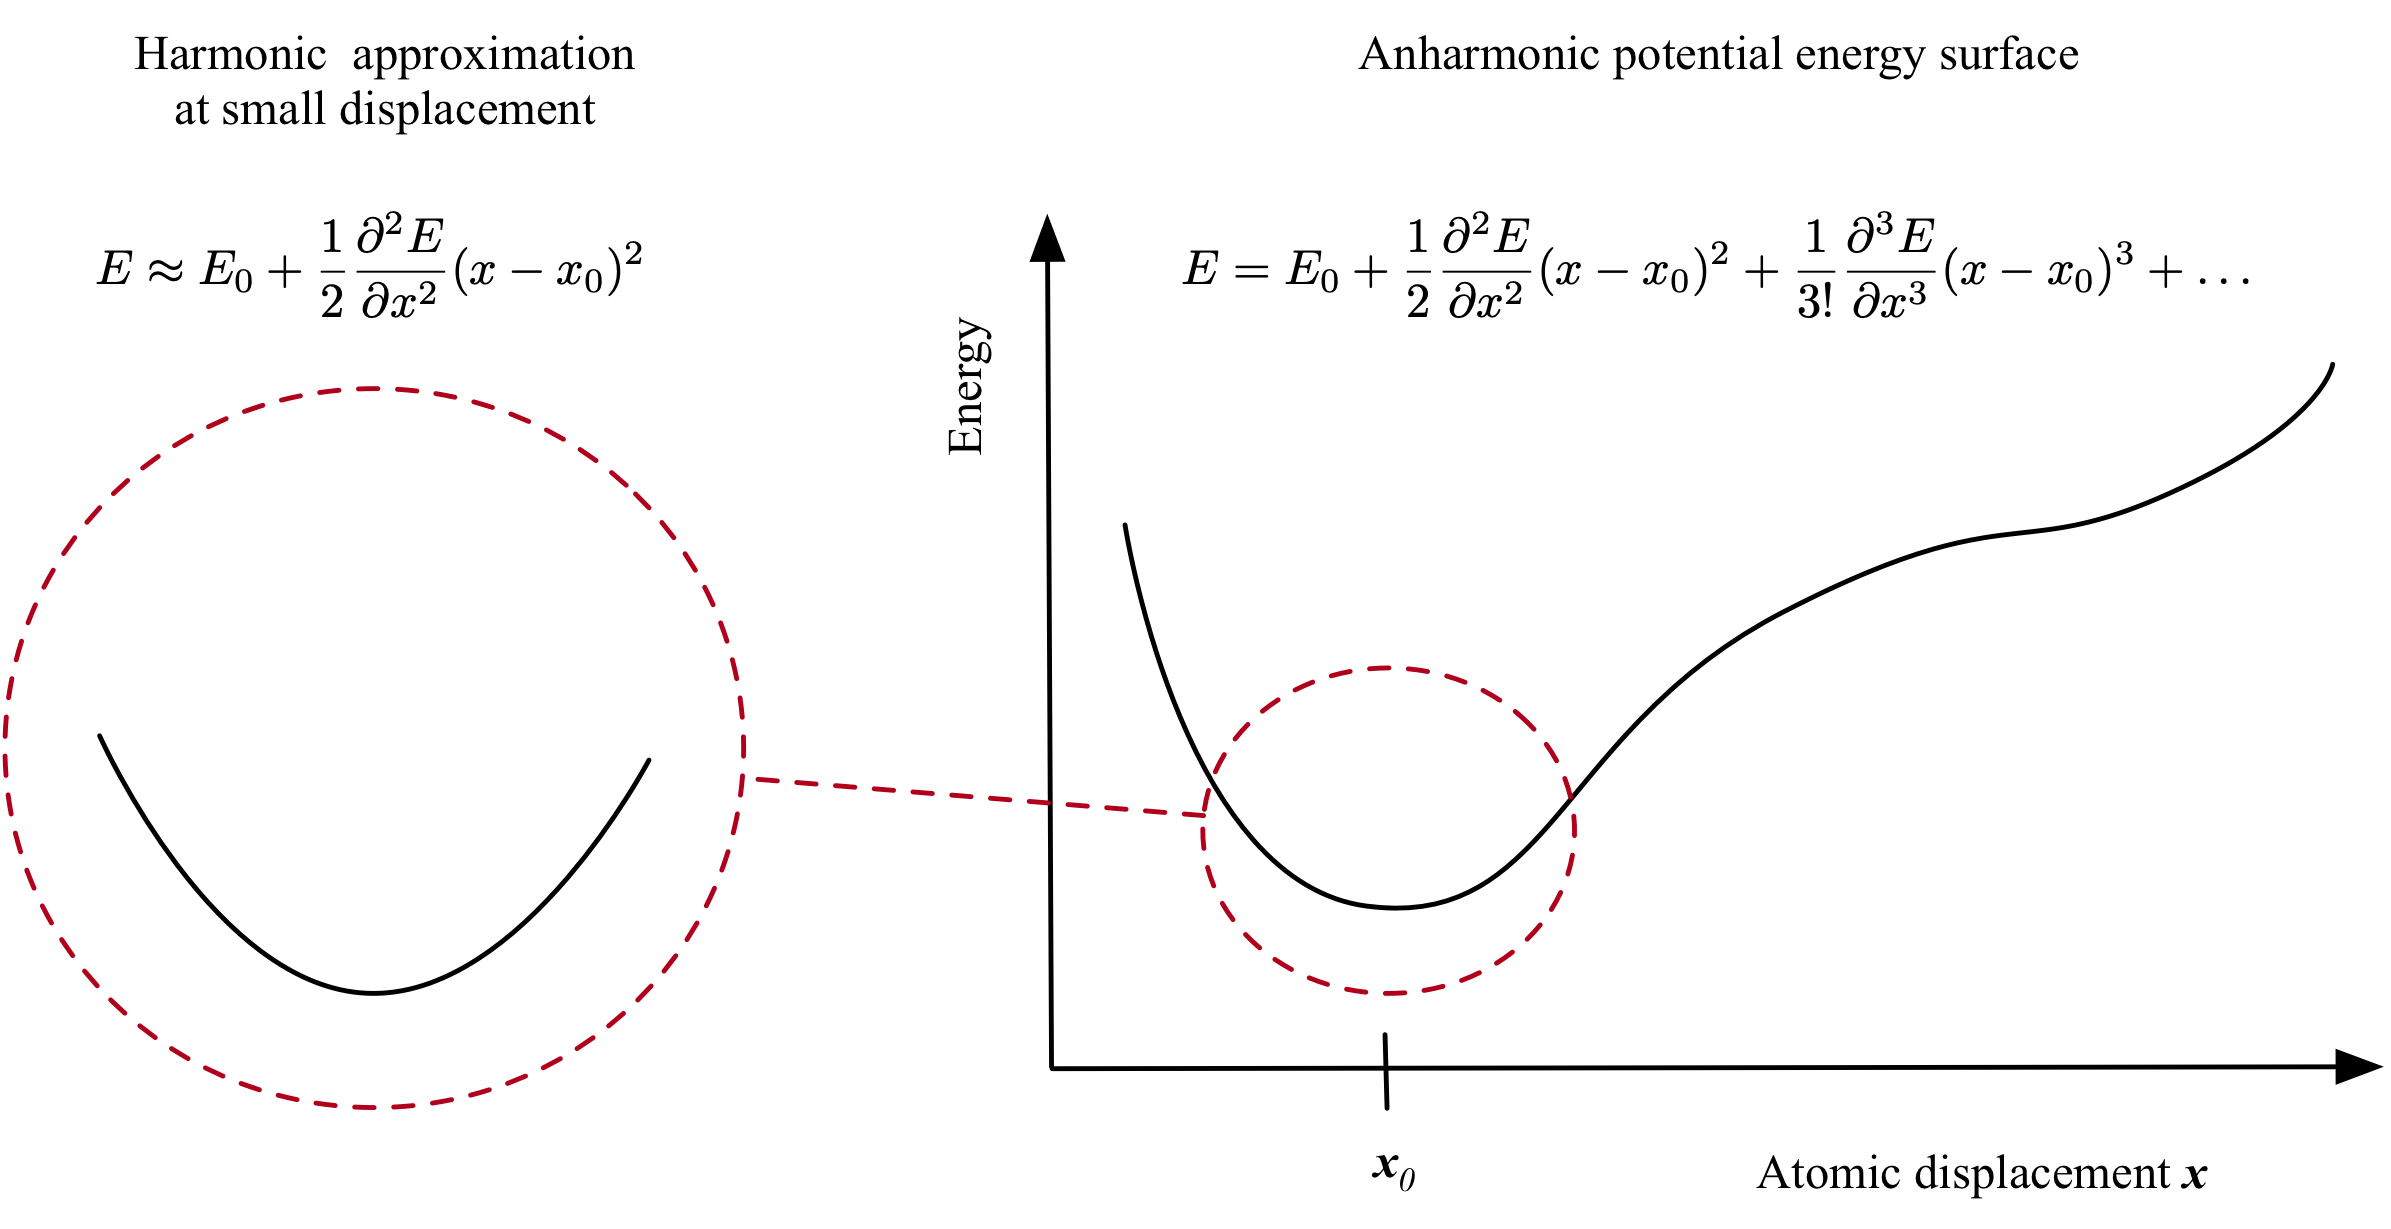
\includegraphics[width=0.8\columnwidth]{figures/ch3/harmonicregime.png}
  \caption[Crystal potential energy expanded with respect to atomic displacement]{The crystal potential energy can be expanded in powers of atomic displacement $x-x_0$, where $x_0$ is the equilibrium position. At small displacements, the anharmonic terms (third order and above) can be ignored, giving the harmonic approximation. For larger displacements, higher order anharmonic terms must be considered. The crystal lattice is relaxed so that all forces on the atoms are zero and there is no first order force term.}
  \label{harmonicregime}
\end{figure}

%important to understand crstal stabilit as the vibrational energy and entropy enter the Gibbs free energy
% - Partition function ---> bridge function kTlnZ (bridges micro and macro thermodyamics) to get helmholtz free energy. need vibrations to get temperature dependent energy and stability as a function of temperature.

% We know this affects electrical and optical properties – look at the peak shift in energy and peak broadening ith temperature.
% % - model for vibrations (harmonic approximation) ---> vib freq and displacement patterns (vibrational spectra) and from that IR/raman, free energies (T) - phase change. all stuff you couldnt get with standard electronic structure
% thermodynamics requires phonons, (helmholtz free energy)


% - What information can we get from phonons? 
% Thermodynamic quantities at low temperature: heat capacity, entropy, free energy, zero-point,
% Phase transitions from the Gibbs free energy,
% Conductivity,
% Infromation about lattice instabilities in the form of imaginary frequencies,
% Elastic tensor from the q to zero limit of phonon dispersion,
% Thermal expansion coefficient,
% Temperature dependence of the bandgap,
% Electron phonon coupling strengths,
% Static polarization

% - Experimental evidence:
% Measured directly with inelastic scattering,
% IR and Raman spectroscopy


% - For small amplitudes we consider a simple harmonic motion. phonon modes are uncoupled and have infinite lifetime.
% - At larger amplitudes we must consider anharmonic motion. phonons can be created and destroyed, have a lifetime and give access to new properties.
% - Extent of Anharmonicity depends upon how much of the potential energy space you are exploring ((tie in with perturbative and non-perturbative regime skethc). At low T you may be exploring harmonic potentil like minima, at High T you may be beyond this minima
% - Adiabatic approximation: Can thin of electronic wavefunction for eignstate of nuclei fixed in position.


% - The motions are determined by atomic forces. For a 1D system with a single mass or with two masses (lattice with basis) we can solve analytically. Otherwise these can be determined through DFT calculations (Hellman Feynmann theorem), producing a force constant matrix. 

% - Table with the approximation and the properties you can get and codes which implement....
% - quasi-harmonic:properties as a function of volume.helmholtz as function of temeparture  - at some point it is favourable to have a different volume . Free energy as function volume for several tempatures and the fit an equation of state. 
% - Then you can get the bulk modulus, heat capacity constant pressure, gibbs free, gruneisan, volumetric thermal expansion.use to get properties at finite T - use the structure which minimises for a particular temp.
% - Thermal expansion coefficients, system anharmonicity (e.g. modal grun parameters) and the temperature-dependence of other properties can be calculated in the quasi-harmonic approximation (QHA). 
% Here the lattice dynamics is harmonic at a given temperature; however, the cell volume is scaled by thermal expansion to give the first-order contribution of finite temperature effects. 
% 2: frequency and eigenvectors
% 3: phonon linewidths / spectral lifetimes
% 4: anharmonic frequency shifts
% https://thelostelectron.wordpress.com/

\subsection{Harmonic approximation} \label{harmonicapprox}

In this section I connect, using a minimum amount of mathematics, an expression for total lattice energy with the force constant matrix (which can be calculated using DFT calculations). For a more complete derivation I refer the reader to Section 2.2 of Reference \cite{Hayes1985}.

If the atomic displacement from equilibrium is small, the total energy can be Taylor expanded in the form\autocite{Hayes1985} 
\begin{align} \label{taylorexpansion}
E&=\textrm{kinetic energy}+\textrm{potential energy} \\
&=\sum_i\frac{1}{2}M\dot{x}_i^2+\sum_{ij}\frac{1}{2}\textbf{x}_i\cdot\textbf{A}_{ij}\cdot\textbf{x}_j+\textrm{higher-order terms},
\end{align}

where it is assumed that the structure is relaxed and forces are equal to zero so that there is no term linear in $\textbf{x}$. The harmonic approximation ignores the higher order terms in Equation \ref{taylorexpansion}. For these harmonic systems there exists a basis set so that $\textbf{A}_{ij}$ is diagonal and the oscillators are independent of one another:
\begin{align} \label{independentoscillators}
&=\sum_j\frac{1}{2}\tilde{M}\dot{Q}_j^2+\sum_{j}\frac{1}{2}\tilde{\textbf{A}}_{j}Q_j^2,
\end{align}
where the linear transformation has cast coordinates $x$ into $Q$.
The general solution to this system of equations for an $N$-atom unit cell in three dimensions is a superposition of $3N$ normal modes of vibration, each with its own frequency and eigenvector.
To calculate the normal modes Newton's second law, $F=ma$, is applied. For crystalline solids we take advantage of symmetry and seek normal modes $\textbf{e}(\textbf{k},t)$ that for a chosen wavevector $\textbf{k}$ are a linear combination of a relative displacement within the unit cell ($\textbf{u}_0(i,\textbf{k})$), a phase that depends on the origin $\textbf{R}_I$ of cell $I$ ($\textrm{exp}(i\textbf{k}\cdot \textbf{R}_I)$), and an oscillation in time of well defined frequency $\omega(\textbf{k})$ ($\textrm{exp}(i\omega(\textbf{k})t)$):
\begin{equation} \label{normalmodes}
\textbf{e}(\textbf{k},t) = \textbf{u}_0(i,\textbf{k})\textrm{exp}(i\textbf{k}\cdot\textbf{R}_I)\textrm{exp}(i\omega(\textbf{k})t).
\end{equation}
For displacements of this form, Newton's second law has consistent solutions only if the following secular equation is satisfied:
\begin{equation}
\textrm{Det}||\sum_J A_{\alpha\beta}(iI,jJ)\textrm{exp}(i\textbf{k}\cdot\textbf{R}_J)-M_i\delta_{ij}\omega^2(\textbf{k})||=0,
\end{equation}
where the first term in the determinent is the dynamical matrix. The dynamical matrix is built from the force constant matrix $A_{\alpha\beta}$:
\begin{equation} \label{forceconstant}
\textbf{A} = 
\begin{pmatrix} 
\frac{\partial^2E}{\partial x_1^2} &\frac{\partial^2E}{\partial x_1 \partial x_2} & \cdots & \frac{\partial^2E}{\partial x_1 \partial x_n}\\
\frac{\partial^2E}{\partial x_2 \partial x_1}&\frac{\partial^2E}{\partial x_2^2} & \cdots & \frac{\partial^2E}{\partial x_2 \partial x_n}\\
\vdots & \vdots & \ddots & \vdots \\
\frac{\partial^2E}{\partial x_n \partial x_1}&\frac{\partial^2E}{\partial x_n \partial x_2} & \cdots & \frac{\partial^2E}{\partial x_n^2}\\
\end{pmatrix}
\end{equation}

The normal mode frequencies $\omega(\textbf{k})$ are roots of the secular equation \ref{normalmodes} and can be found through matrix diagonalisation. Plotting the frequency $\omega$ against wavevector $\textbf{k}$ for a lattice with a periodicity of length $L$ gives a bandstructure plot with a periodicity of $\frac{2\pi}{L}$.   %check that a is correct for lattice length 

The discussion so far has only used classical mechanics. To introduce quantum effects we recognise that the harmonic lattice vibrations are analogous to a quantum simple harmonic oscillator and so will be restricted to certain energy values $E_n = \hbar\omega(\textbf{k})(n+\frac{1}{2})$.
The discrete (quantised) unit of energy $\hbar\omega(\textbf{k})$ is a phonon quasiparticle that corresponds to a collective excitation of the crystal lattice.
% The phonons of energy hbar omega have exact energy so cannot be localised in space: formed of delocalised plane waves
% But can construct localized packet using modes of different fequency. Can then treat phonons as localised particles. E = hbar omega. K is the crystal momentum .
% Phonons are bosons, not conserved. They can be created and destroyed. 
% once got eigencevtors nad freuencies have access to toher props via partition function

\subsection{Anharmonicity} \label{anharmonicapprox}

Anharmonic atomic motion is described by the higher order terms in Equation \ref{taylorexpansion}.
The third order term accounts for phonon-phonon scattering which, due to the conservation of energy and momentum, is a three particle process (Figure \ref{thermalconductivity}).\autocite{Lundstrom2000}

The linear boltzmann transport equation (LBTE) describes a thermodynamic system out of equilibrium. Solving the LBTE under the single mode relaxation time approximation gives an expression for the lattice thermal conductivity $\kappa$. %cite https://arxiv.org/pdf/1501.00691.pdf
The phonon-phonon scattering rate determines the phonon lifetime $\tau_\lambda$ which is a key quantity in the expression for $\kappa$:
\begin{equation}
    \label{thermalconductivity}
    \kappa=\frac{1}{NV_0}\sum_\lambda C_\lambda v_\lambda \times v_\lambda \tau_\lambda,
\end{equation}
where $N$ is the number of unit cells in the crystal, $V_0$ is the unit cell volume, and $C_\lambda$, $v_\lambda$ and $\tau_\lambda$ are the mode-dependent heat capacity, group velocity and lifetime respectively. $C_\lambda$ and $v_\lambda$ can be calculated using the harmonic approximation. To quantify the strength of the anharmonic phonon interactions that determine $\tau_\lambda$ it is necessary to calculate a third-order force constant matrix. This is often at high computational cost; in Reference \cite{Whalley2016} 41,544 DFT calculations were required to calculate the thermal conductivity of a 96-atom unit cell.
% -  can reduce the cst by just considering the phase space (broido talk, laptop notes)

Lattice anharmonicity can also be used to describe materials with dynamic disorder. In the halide and oxide perovskites the onset temperature for dynamic disorder is determined by the depth of the double well potential energy surface (Figure \ref{thermalconductivity}).\autocite{Yang2017}
Chapter \ref{ch:5-epcoupling} calculates the coupling between the anharmonic double well phonon modes and electronic states in MAPI.
 % - anharmonicity schematic under visuals: Si, PbTe, SrTiO3% - Anharmonicity also needs to be considered according to material (schematic here)
% for some vobrations compression and extension will not be equal curvature. talk about % - harmonic approximation expects the energy to increase as you push along the mode.imaginary frequency because $w^2$ is negative.
% - dynamic stability if all positive
%- mechanism for some phase transitions is where phonon mode becomes imaginary at a transition temperature
% frozen phonon approximation


% - Anharmonicity most important when under high pressure or high temperature (bouchert) which is often the case for geophysical applications.
% - Navaneeth : assessing how higher order anharmonicity can aggect htermal conductivity. In Diamond the 4 phonon phase space is 10x that of 3-phonon. In Bas it is 100X that of 3-phonon phase space. We must then also consider the scattering strength (can only consider the scattering rate of those with a large phase space). The size of these phase spaces are huge. For example, Bas which is in the zincbelnde structure has 6 polarisations. If each done explicitly there would be $9x10^ 3$-phonon calculations, for 4-phonon processes there would be $2x10^12$!!!  So instead temperature-dependent ensembles are used (where all atoms are moved at the same time, calculated from explicit 2nd order force constant calculation) and then used to fit 3rd and 4th order force constants to.



\begin{figure}[h]
\centering
  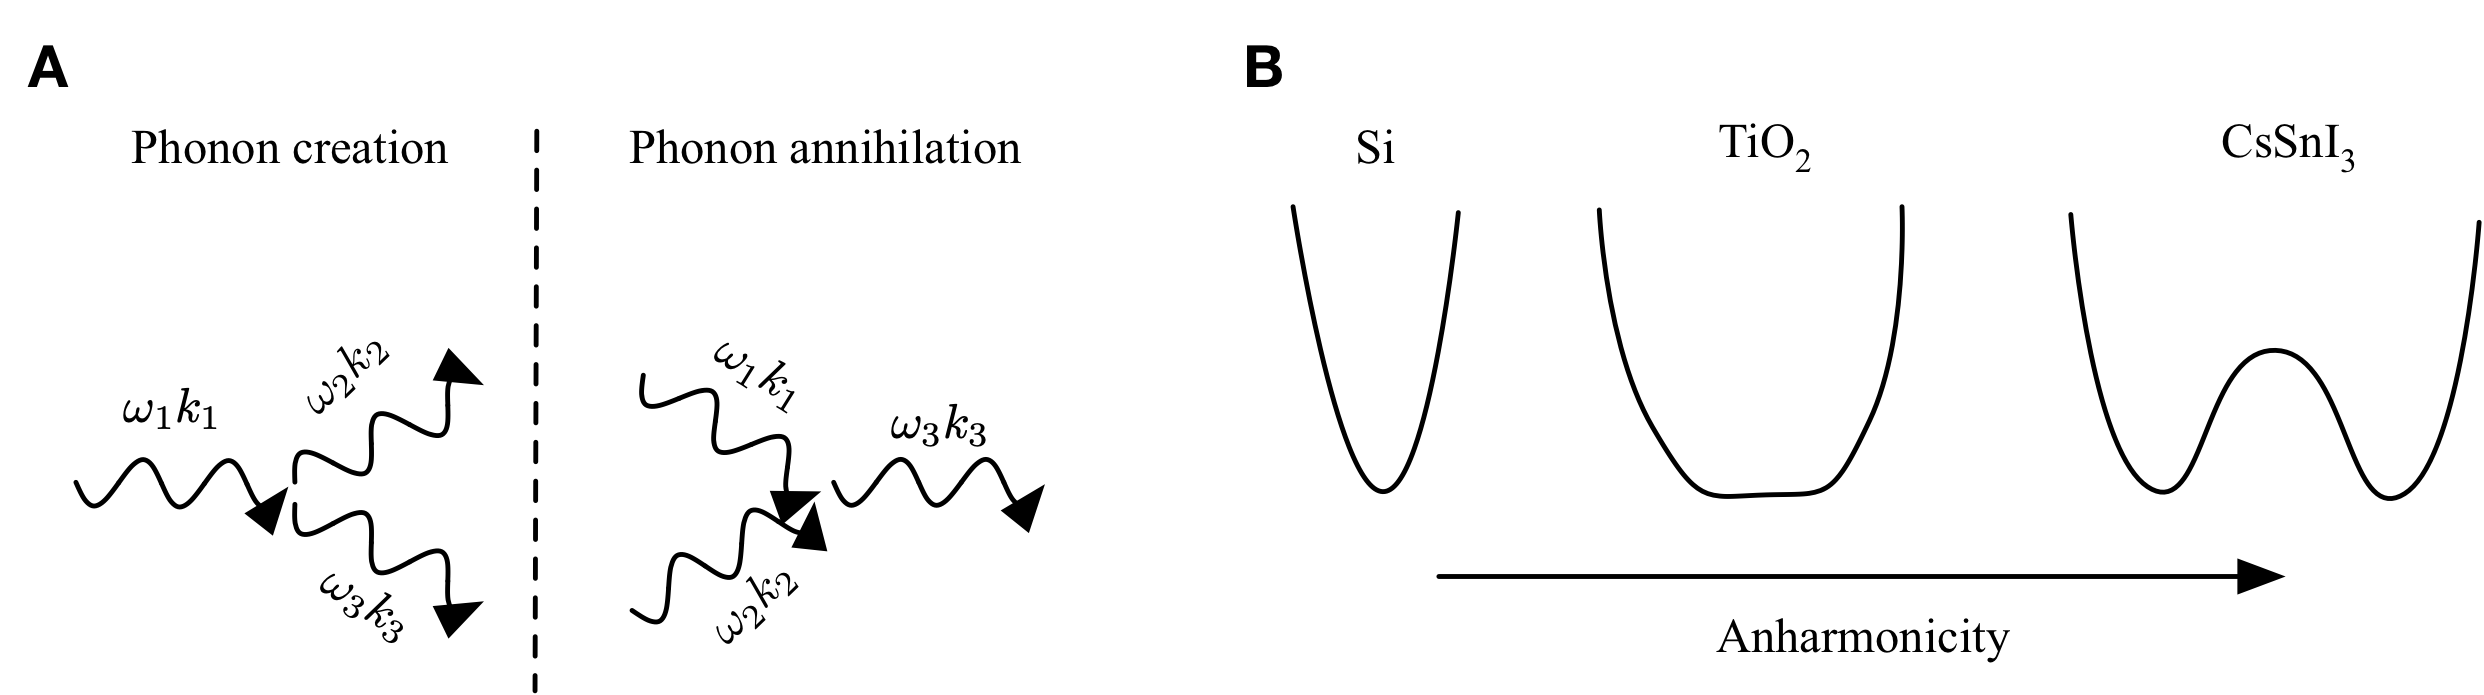
\includegraphics[width=1.0\columnwidth]{figures/ch3/anharmonicity.png}
  \caption[3-phonon processes and anharmonic potential energy surfaces]{A) Energy and momentum are conserved during the creation or annihilation of phonons, so these are three-phonon processes (or higher); B) Some materials, such as silicon (Si) are well-described by a harmonic potential energy surface at typical solar cell operating temperatures. However other materials with dynamic disorder, such as the organic and inorganic perovskite halides, have highly anharmonic double well potentials.}
  \label{harmonicregime}
\end{figure}  %include phonon-phonon scattering schematic? the third regime where important is given in the other figure, at high temperature %cite ruoxi work



\subsection{Finite displacement method} \label{finitedisplacement}

There are a number of ways to calculate the second order force constant matrix in Equation \ref{forceconstant} including: the finite displacement method; density functional perturbation theory; ab-initio molecular dynamics and compressed sensing lattice dynamics.
In this work the finite displacement method (also known as the direct or supercell method) is used: a single atom is displaced a small distance from its energetic minimum and there is a self-consistent electronic structure optimisation to calculate the resultant forces. The maximum number of displacements for a system with $N$ atoms is $6N$, although this is reduced through symmetry. 
To consider phonon wavelengths greater than the unit cell length a supercell is required, and all forces must be well converged (typically to less than \SI{0.01}{\electronvolt\per\angstrom}).

%negatives of this approach: no long range forces beyond hte supercell (polar materials), no anharmonicity .  %positive - highly parallelisable

% - Note that the  eigenvalue equation for the dynamical matrix is gotten from fourier transform
% Of the taylor expansion of the crystal potential.
% - force constant matrix . then construct dynamical matrix - -> wavevector. then diagonalise - the eigenvectors and eigenvalues. do a schematic for this process. then two ways to get to the dynamical matrix.

% - There are a multitude of ways to calculate these force constants: explicitly (finite difference, DFPT for 3rd or 4th orders), empirical potentials (TDEP), compressive sensing lattice dynamics or beyond perturbation (AIMD,PIMD,SCAILD, variational methodslike SSCHA developed by Ion Errea).
% - perturbation theory- dynamical matrix directly. no supercell and more accurate but constrained which functionals and pseudopotentials you need.

% schematic of workflow: input structure, create displacements, calculate forces, calculate dynamical matrix, diagonalise

% phonon workflow

% in this work the finite displacement approach is used as implemented in...
% For derivatives we exploit the hellman-feynam theorem and use finite differences % - Force constant via finite displacement - displace small and calculate force. Simple, general and can split into small jobs (parallelise). 
% AKA "supercell","direct" or "frozen phonon" 
% - phonons can have a wavelength longer than the size of the supercell - need to capture the longer wavelength. but need supercells. use phonopy. Maximum is 6N displacements but this is seriously reduced by symmetry. (spglib)
% - Need good relaxation: don't skimp on the forces, cutoff or k-points.
% - PBEsol for reproducing lattice constants and phonons (Jonathan 2015 J.Chem. Phys)

% - See Jonathans talks

\section{Summary}

In this chapter I have introduced the key concepts that underly DFT, and the post-processing steps required to calculate the defect and vibrational properties of a crystal. 
Much of solid state physics is built upon the idea of a translationally invariant crystal, so it should come as little surprise that additional steps are needed to describe defects that break translational symetry and work against the fundamental assumptions of the theoretical framework.
In contrast, phonons at the gamma point preserve the underlying crystal symmetry, but additional steps are needed to build the force constant matrix from multiple DFT calculations.
In this chapter I have presented the defect and vibrational calculations separately. However in Chapter \ref{ch:6-defects} I also combine the two approaches, and calculate the vibrational properties of the iodine interstitial defect in MAPI. 
%A discussion about how a point defect perturbs the vibrational sub-system of a bulk material is included in that final chapter.
%: LW - could we add here that solid state physics of crystalline materials is not really built for defects as they assume perfect translational symmetry, which the defects break ---> which makes modelling defects a continuing challenge for theory and simulation (as we are working "against" the fundamental assumptions of the framework).
% - defects are demainding and computational expensive .n To avoid computationally expensive defect calculations descriptors have been built on the idea of ‘defect tolerant’ materials: http://pubs.acs.org/doi/pdf/10.1021/acs.nanolett.5b04513
% in fact I combine defect and phonon calculations in final chapter



\include{text/ch3-effmass}
\include{text/ch3-epcoupling}
\include{text/ch3-defects}

%%% DEBUGGIN'
%\begin{table}
\begin{tabular}{llll} %@{} removes space to the vertical edges
\toprule   
Material & $\frac{m^*}{m_0}$ & $\epsilon_0$ & $E_1 (meV)$ \\
\midrule
MAPI & 0.15\autocite{Frost2014b} & 25.7\autocite{Frost2014b} & 3 \\
Si & 0.45\autocite{Hava2007} & 11.7\autocite{Hava2007} &  45 \\
CdTe & 0.11\autocite{Wang2007} & 10.2\autocite{Madelung2003} & 14 \\
\bottomrule
\end{tabular}
\caption[Donor defect levels in \ce{CH3NH3PbBr3}, Si and CdTe]{\label{tab:defectlevels}The first shallow donor defect level in \ce{MAPI}, \ce{Si} and \ce{CdTe} calculated from effective mass theory using Equation \ref{hydeqn}. The dielectric constant $\epsilon_0$ can be considered an important descriptor for photovoltaic materials as several important properties (e.g. rate of impurity scattering) scale with its square.}
\end{table}

%%%%%% LW - closing remarks

\begin{savequote}[8cm]
“I don't know where I'm going from here, but I promise it won't be boring.” 
  \qauthor{--- David Bowie}
\end{savequote}
\begin{closing}
    The subject of this PhD thesis has been to investigate distortions (in the form of nonparabolic electronic bandstructures and anharmonic potential energy surfaces) and defects (in the form of the iodine interstitial) in hybrid halide perovskites. There are three main components in this work:

First I assessed the impact of band nonparabolicity on transport and optical properties at high carrier concentration. \textbf{I have shown that effective masses of PV materials are not constants and that this leads to a reduction in carrier mobility at high carrier concentration}. I have written and published a software package (Appendix \ref{app:1-effmass}) so that researchers can apply my methodology to their system of interest; application to materials that operate at high carrier concentrations, such as transparent conducting oxides or thermoelectric materials, could be particularly interesting.

I then considered the consequences of electron-phonon and phonon-phonon coupling in the hybrid halide perovskite \ce{CH3NH3PbI3}. \textbf{My results show that there is strong coupling between the electronic states at band edge and the anharmonic phonon modes associated with tilting of the inorganic octahedra}. Using parameters derived from the Fr\"{o}lich polaron model, \textbf{I have found that the cooling of photoexcited, above bandgap carriers is limited by the ultralow thermal conductivity of the perovskite lattice and that cooling to equilibrium happens over 100s of picoseconds}. This compares well to the experimentally observed time scale of slow carrier cooling.

Finally, I studied the properties of the iodine interstitial defect. \textbf{I predict that holes are self-trapped at the iodine interstitial to form a H-centre defect ($\mathbf{I_2^-}$), and that the rate of hole trapping is X}. This line of research prompts a number of questions for future work:
\begin{itemize}
    \item Does hole capture lead to device degradation? Hybrid halide perovskites have an ultra-low thermal conductivity\autocite{Whalley2016} which, when combined with fast carrier trapping (where electronic energy is converted to lattice energy), could lead to a build up of highly localised heat. This local heating could accelerate device degradation; experimental reports show that decomposition of MAPbX (X = I, Br) can be triggered by a raman laser.\autocite{Ledinski2015}
    \item Do stochiometric iodine pairs form V-centres? It is energetically favourable to form V-centres in metal halides such as KCl,\autocite{Castner1957} but formation of this defect in the the metal halide perovskites has not been considered. If favourable, the V-centre will form in high concentrations as it is a stoichiometric defect (requires no excess or missing atomic species). The long diffusion length but mediocre mobility of charge carriers in hybrid halide perovskites\autocite{Brenner2015} supports the existence of the V-centre, although this could also be accounted for by other types of polaron formation. 
    \item Is defect energy depth a good measure of wavefunction localisation? In the literature a ``deep'' defect state (with a charge transition level towards the centre of the bandgap) is often correlated with highly localised charge. This correlation between the defect depth and localisation is often assumed (with the terms sometimes used interchangeably), but to my knowledge there is no systematic study of this relationship. A potential study could consider e.g. anion vacancies across CdTe, GaAs and MAPI.
\end{itemize}

During my PhD studies I have made key datasets and analysis scripts openly available through the GitHub platform. My reasons for doing so are three-fold: for increased reproducibility; to reduce duplication of effort and so make efficient use of public money and researcher time; and to promote my work. Reproducibility is surprisingly difficult to achieve -- I have found that publishing software is not enough, and that software documentation and testing is needed to ensure that others can independently reproduce my results. It has taken time to develop the skills needed to write, document, test and publish code, but I consider it time well spent.

In the first chapter I motivated this work with reference to global warming. However it is clear that efficient photovoltaic materials alone will not slow global warming, and that the larger picture must be considered. For example, if PV is to provide a large proportion of our energy supply, it will need to be combined with large scale energy storage networks. If we are serious about climate change as the motivating factor, it may be that we have to look beyond science, as some claim that it is the political will, rather than technological solutions, that are lacking. 

If, however, we believe that scientific understanding is an end in itself, there is plenty of motivation for further research into hybrid perovskite materials. In addition to the open questions listed previously, there is a technologically important and fundamentally interesting question relating to the metal B-site species: is it possible to replace lead with a non-toxic element? Efforts so far have failed as the chemical structure of lead is such that the dispersive $s$-orbital is active in the valence band, leading to excellent transport properties that cannot be reproduced with tin on the B-site, for example.
There are many opportunities ahead as we pick apart the relationship between organic and inorganic components, electronic and ionic states, as well as order and disorder in this complex family of materials.

% it is a complex material that is simple to process

%not touched on is toxicity and drive to replace lead.The lead is important for transport properties. The lead is in a 2+ charge state. This means it has the chemical structure 6s2 6p0. This means that the dispersive s-orbital is active in the valence band. So when charge electrons are exautocited to the conduction band the holes are in a dispersive valence band and so can provide ambi-polar transport. The iodine provides dispersive conduction band edge (rom real-space structure can see there must be hybridization as there is no Pb overlap). Pb has the edge over Sn based compounds as the s electrons in Pb are deeper down and so harder to remove. In Sn based perovskkites the Sn2 wants to form Sn4 which kills the transport (dispersion) and leads to breakdown of the material (formation of different phases) – the Sn wants to oxidise.


\end{closing}

%% APPENDICES %% 
% Starts lettered appendices, adds a heading in table of contents, and adds a
%    page that just says "Appendices" to signal the end of your main text.
\startappendices
% Add or remove any appendices you'd like here:
\chapter{\label{app:1-effmass}effmass: An effective mass package}

\section{Summary}
\label{sec:summary}

Many semiconductor properties depend on the response of electrons to an external pertubation. This perturbation could take the form of an electric field, change in temperature or an applied lattice stress. In a crystal, this response depends on the interaction of the electrons with a periodic potential. The effective mass approximation assumes that the response of an electron in a periodic potential is equivalent to that of a free electron with a renormalised mass (called the ``effective mass''). This makes the effective mass a critical parameter in models for the optical and transport properties of a semiconductor.

The effective mass has a number of definitions, depending on the perturbation under consideration. The conventional definition of effective mass is inversely proportional to the second derivative of electron energy with respect to electron momentum \autocite[p.~227]{Ashcroft1976}. This allows the effective mass to be easily calculated from ab-initio band structures, and there are existing codes which have implemented this (see section ``Related packages'' below).

We must approximate the band structure with a parabola for the previous definition to be valid \autocite{Ariel2012}. However, this approximation breaks down when there is a high concentration of electrons in the material - when, for example, the material is doped or excited under a laser. Instead, we can then approximate the band structure with the Kane quasi-linear dispersion \autocite{Kane1957}, and the definition of effective mass is adapted accordingly.

effmass \autocite{Whalley2018b} is a Python 3 package for calculating various definitions of effective mass from the electronic bandstructure of a semiconducting material. It contains a core class that calculates the effective mass and other associated properties of selected band structure segments. effmass also contains functions for locating band structure extrema, calculating the Kane quasi-linear dispersion parameters and plotting approximations to the true dispersion. Parsing of electronic structure data is faciliated by the vasppy \autocite{Morgan2018} package.

The effmass package is aimed towards theoretical solid state physicists and chemists who have a basic familiarity with Python. Depending on the functionality and level of approximation you are looking for, it may be that one of the packages listed below will suit your needs better.

\section{Related packages}
\label{sec:related}

Effective mass calculations are implemented in a number of other packages:
\begin{itemize}
    \item vasppy \autocite{Morgan2018}: This is installed as a dependancy of effmass. Calculates the effective mass using a least-squares quadratic fit for parabolic dispersions.
    \item sumo \autocite{Ganose2018}: Calculates the effective mass using a least-squares fit for parabolic and non-parabolic dispersions.
    \item emc \autocite{Fornari2012}: Calculates the effective mass tensor using a finite-difference method for parabolic dispersions.
    \item pymatgen \autocite{Ong2013}: This is installed as a dependancy of effmass. Calculates an average effective mass tensor for non-parabolic dispersions with multiple bands and extrema. Also calculates the Seebeck effective mass as defined here.
\end{itemize}

\section{Unique features of effmass}
\label{sec:unique}

To our knowledge, the following features are unique to this package:
\begin{itemize}
    \item easily compare the values of curvature effective mass calculated using multiple numerical techniques (least-squares and polynomial fitting)
    \item tailor the polynomial fitting used to approximate the DFT calculated dispersion: by choosing the order of the polynomial and the energy range to fit over.
    \item visualise the dispersions used to approximate the DFT calculated dispersion
    \item quantify non-parabolicity through the Kane dispersion parameters: effective mass at band-edge and alpha
    \item calculate the optical effective mass assuming a Kane dispersion.
\end{itemize}

\textbf{Acknowledgements}

LW would like to thank Aron Walsh, Benjamin Morgan and Jarvist Moore Frost for their guidance during this project. This package was written during a PhD funded by the EPSRC through the Centre for Doctoral Training in New and Sustainable Photovoltaics (grant no. EP/L01551X/1). The input data used for developing and testing this package was generated using the ARCHER UK National Supercomputing Service. We have access to Archer via our membership of the UK's HEC Materials Chemistry Consortium, which is funded by EPSRC (EP/L000202).



%% include the hot carrier cooling derivations and scripts
%% include exchange correlation functional , alpha value on defect formation energy

%%%%% REFERENCES

% JEM: Quote for the top of references (just like a chapter quote if you're using them).  Comment to skip.
%\begin{savequote}[8cm]
%The first kind of intellectual and artistic personality belongs to the hedgehogs, the second to the foxes \dots
%  \qauthor{--- Sir Isaiah Berlin \cite{berlin_hedgehog_2013}}
%\end{savequote}

\setlength{\baselineskip}{0pt} % JEM: Single-space References

{\renewcommand*\MakeUppercase[1]{#1}%
\printbibliography[heading=bibintoc,title={\bibtitle}]}


\end{document}
